% Chapter X

\chapter{Boiling Bubble Dynamics} % Chapter title

\label{ch:bub_dyn} % For referencing the chapter elsewhere, use \autoref{ch:name} 

%----------------------------------------------------------------------------------------
\minitoc

\section{Introduction}

Boiling bubble parameters are playing an important role in the Heat Flux Partitioning models. For instance, the evaporation heat flux $\phi_{e}$ is directly proportional to the bubble lift-off radius $R_{lo}$ \ref{eq:phie_KP} while the quenching heat flux $\phi_{q}$ depends on the wall area visited by a bubble $A_{q,1b}$ (Eq. \ref{eq:phiq_Basu}) which depends on the bubble sliding length $l_{sl}$, departure raidus $R_{d}$ and lift-off radius $R_{lo}$.

\subsection{Experimental Insights}

Consequently, many experimental investigations have been conducted to further understand the behavior of nucleated bubbles on a wall while facing a liquid flow. In the case of vertical flow boiling, a typical bubble life cycle can be described as follows:

\begin{itemize}
\item Beginning of nucleation, growth while attached to the nucleation site ;

\item Detachment occurring at radius $R_{d}$, from which the bubble will start to slide and accelerate along the wall ;

\item Lift-off from the wall at radius $R_{lo}$ after sliding over a length $l_{sl}$.

\end{itemize}


\begin{figure}[H]

\begin{center}

\subfloat[Bubble sliding visualized and adapted from Maity \cite{maity_effect_2000} at atmospheric pressure.]{
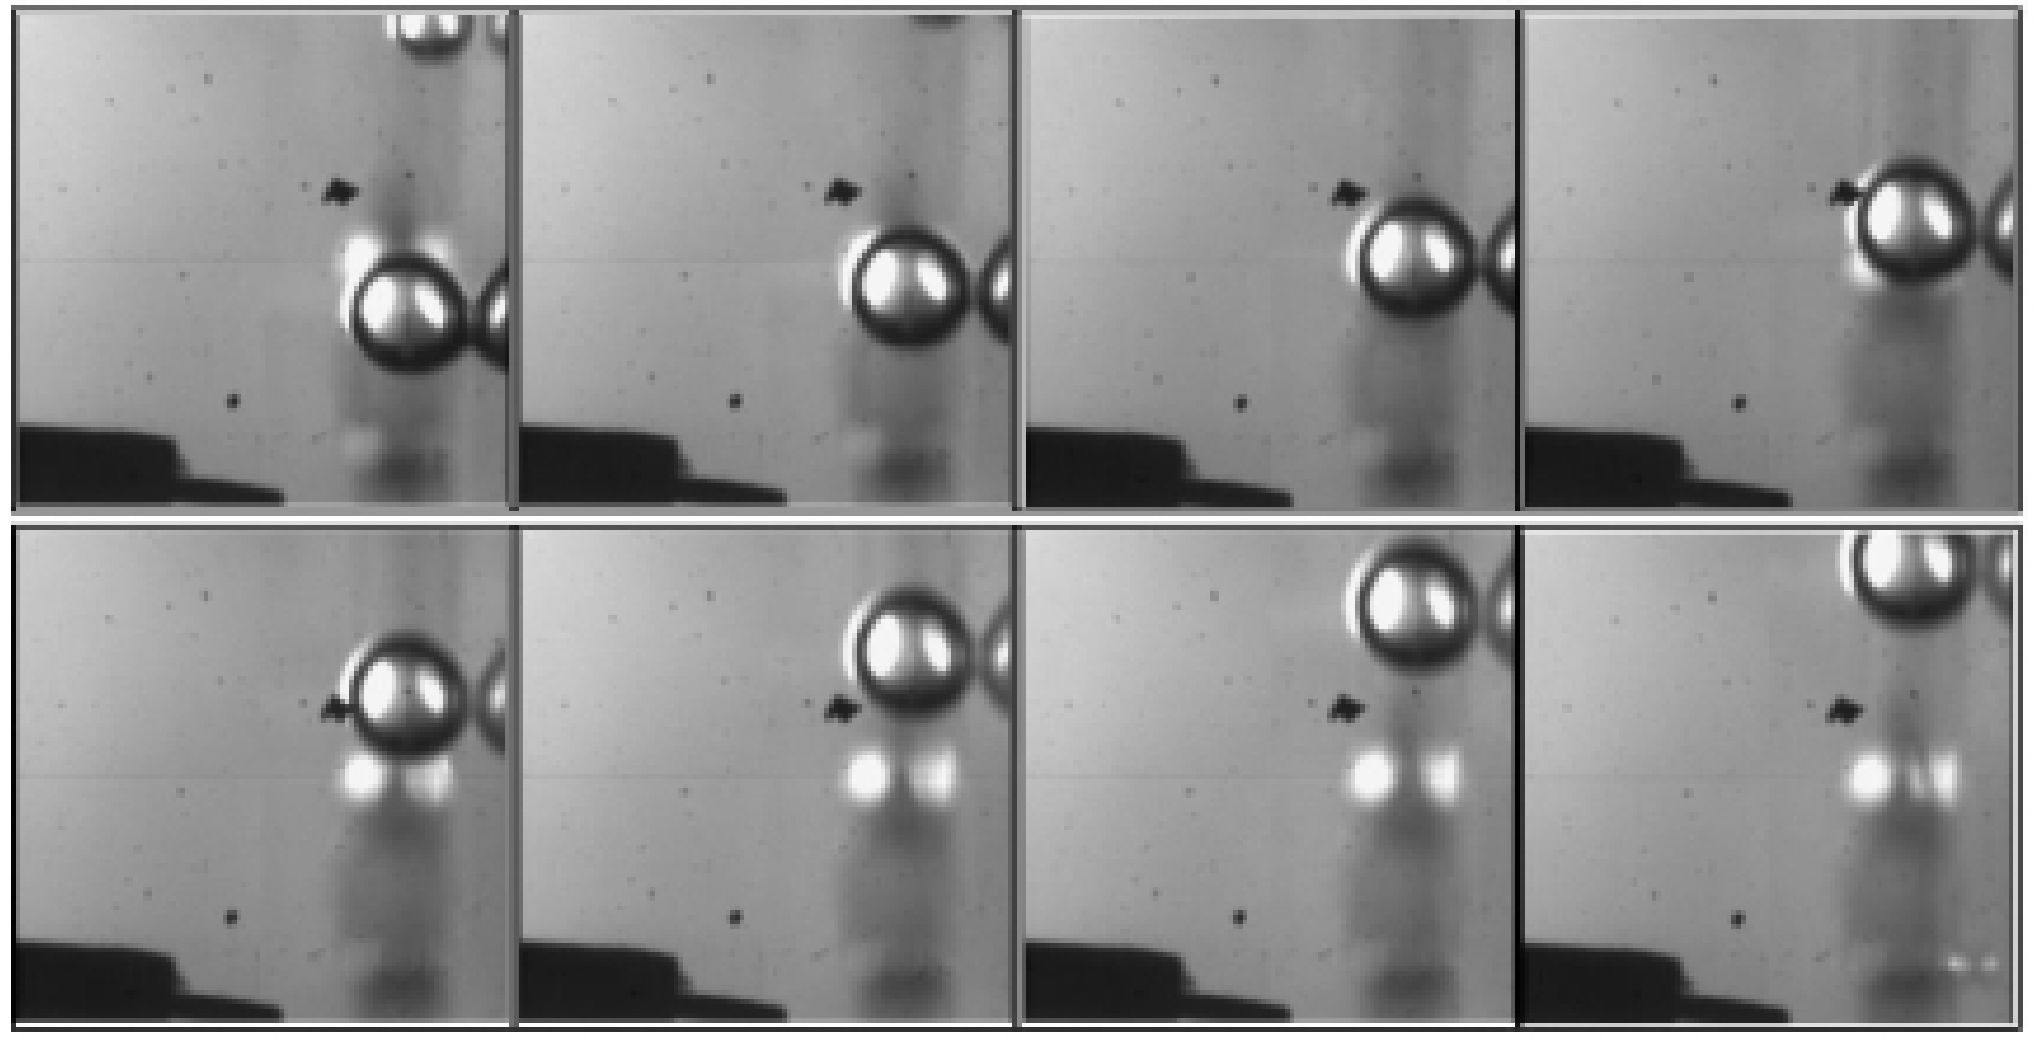
\includegraphics[width=0.6\linewidth]{img/bub_dyn/slide_maity.png}
} 
\\
\subfloat[Bubble sliding visualized and adapted from Kossolapov \cite{kossolapov_experimental_2021} at higher pressure.]{
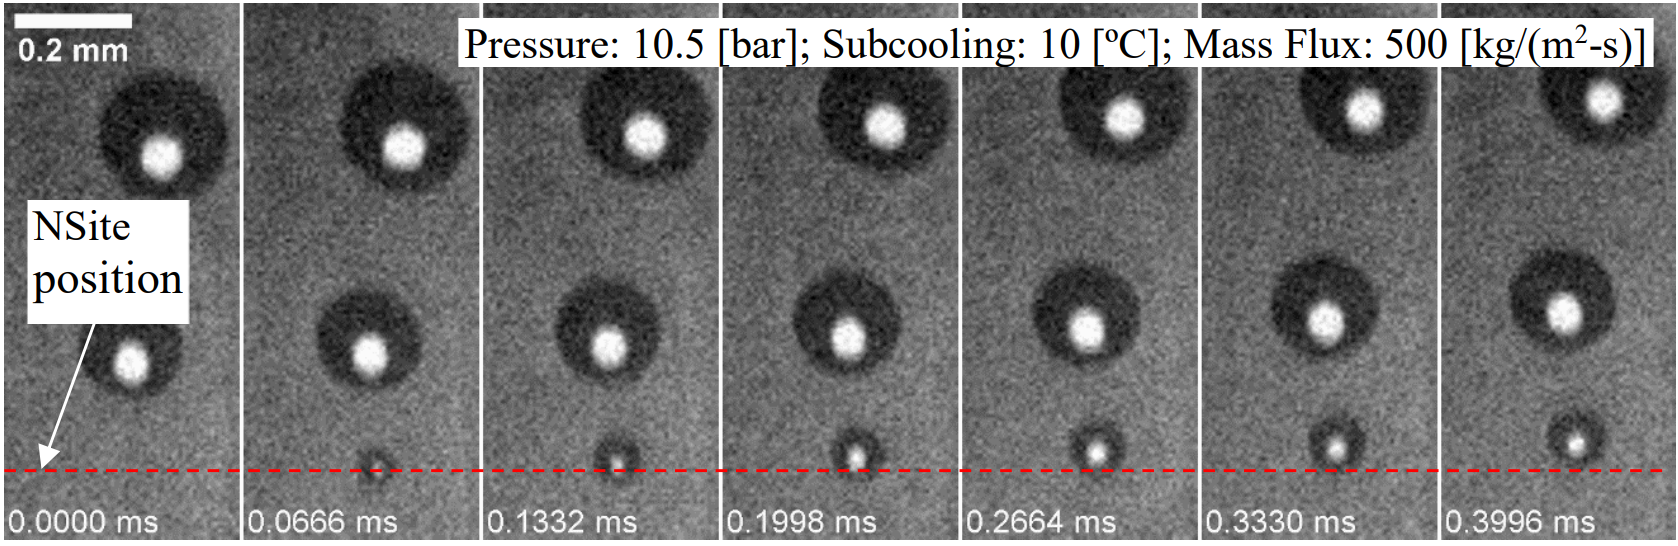
\includegraphics[width=0.6\linewidth]{img/bub_dyn/slide_koss.png}
} 

\end{center}

\caption{Visualization of bubble sliding at various pressures.}
\label{fig:slide_exp_vis}
\end{figure}


This behavior has been supported by many experimental observations who clearly observed three stages (departure, sliding, lift-off) both at low pressure (Maity \cite{maity_effect_2000}, Situ \cite{situ_bubble_2005}, Thorncroft \cite{thorncroft_experimental_1998}, Prodanovic \cite{prodanovic_2006}, Chen \cite{chen_prediction_2012}, Ren \cite{ren_development_2020}, etc.) and high pressure (March \cite{march_1990}, Kossolapov \cite{kossolapov_experimental_2021}). Altogether, those works cover various flow conditions and operating fluids which insist on the generality of this bubble behavior in vertical flow boiling. Examples from the literature of visualizations of bubble sliding at atmospheric and high pressure are reproduced on Figure \ref{fig:slide_exp_vis}.

\npar

The bubble sliding process has also been thermally studied to quantify its impact over the wall heat transfer. Estrada-Perez \etal \cite{estrada-perez_time-resolved_2018} observed the significant thermal impact of sliding bubbles footprints. Kossolapov \cite{kossolapov_experimental_2021} also investigated the sliding of boiling bubbles and measured the magnitude of the transient heat transfer induced by the disruption of the liquid thermal boundary layer in the bubble's wake. Typical experimental observations from those works a reproduced on Figure \ref{fig:slide_thermal_exp}

\begin{figure}[H]

\begin{center}
\subfloat[Instantaneous and time-averaged wall temperature in boiling regime visualized and adapted from Estrada-Pérez \etal \cite{estrada-perez_time-resolved_2018}.]{
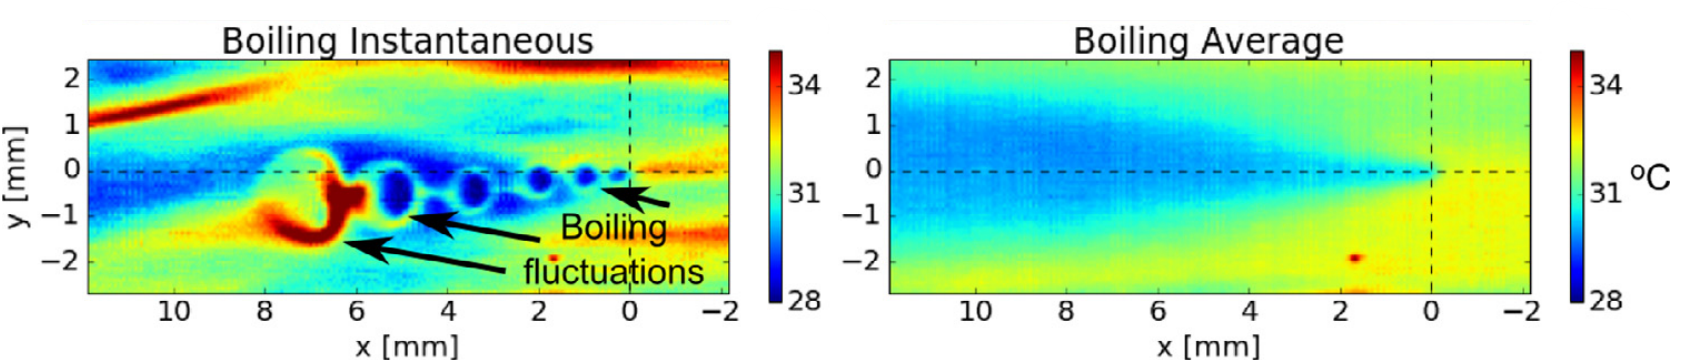
\includegraphics[width=0.8\linewidth]{img/bub_dyn/slide_thermal_estrada.png}
}
\\
\subfloat[Transient conduction induced by sliding bubbles visualized and adapted from Kossolapov \cite{kossolapov_experimental_2021}.]{
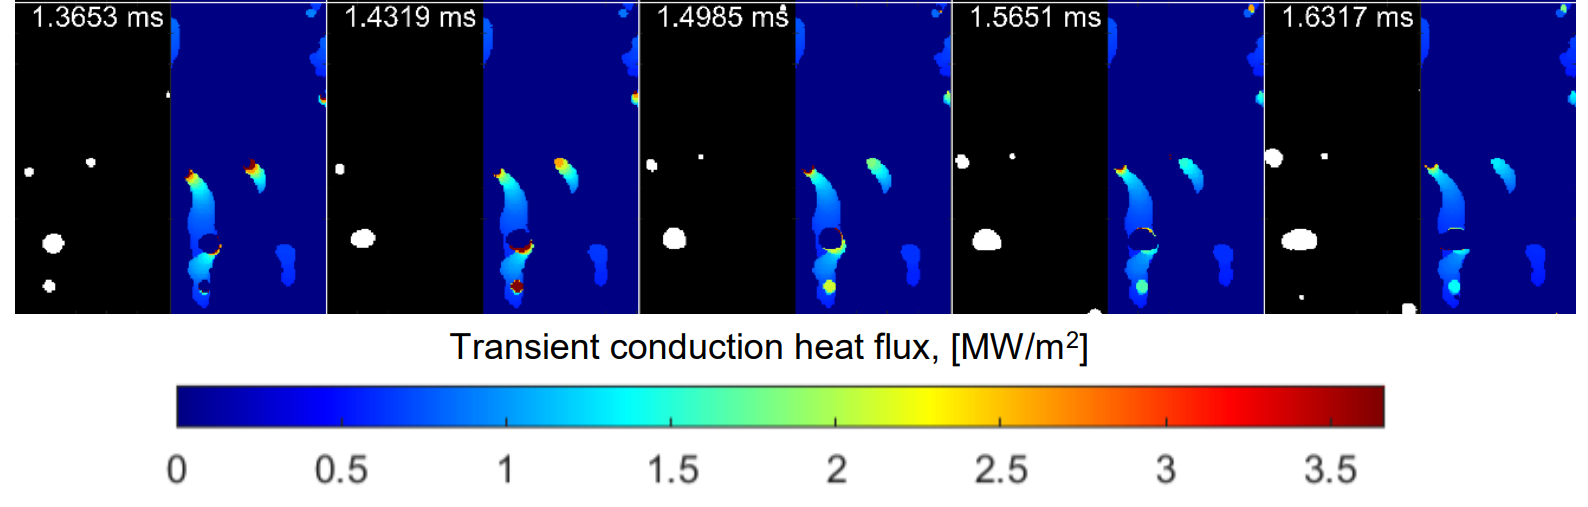
\includegraphics[width=0.8\linewidth]{img/bub_dyn/slide_thermal_koss.png}
}
\end{center}

\caption{Visualization of bubble sliding thermal impact.}
\label{fig:slide_thermal_exp}
\end{figure}


Those experimental observations highlight the significant magnitude of the transient heat transfer triggered by bubble movement on the wall that can represent up to 40\% of the total wall heat flux \cite{kossolapov_experimental_2021}. All the aforementioned observations are summed-up on Figure \ref{fig:sketch_bub_VFB}. 

\begin{figure}[h!]
\centering
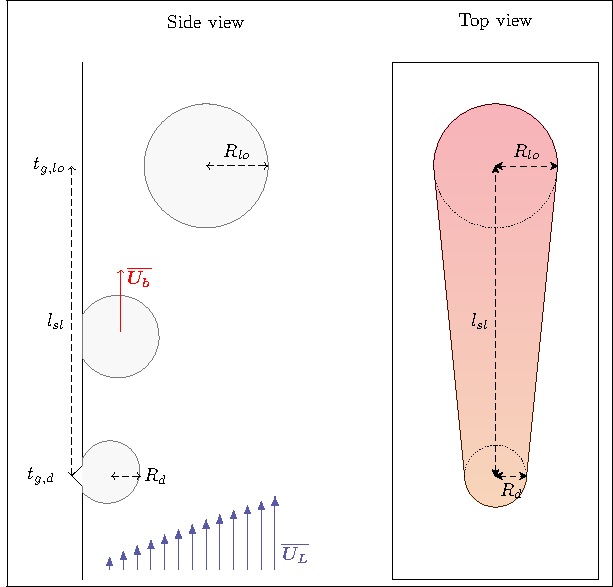
\includegraphics[width=0.65\linewidth]{img/bub_dyn/bub_life_VFB.pdf}
\caption{Sketch of a typical bubble lifetime in vertical flow boiling. Left depicts a typical side view of the heater with identification of departure, sliding and lift-off. Right depicts a top view of the heater, exhibiting the area that will undergo transient heat transfer.}
\label{fig:skecth_bub_VFB}
\end{figure}

\npar 

Predicting the HFP in vertical flow boiling thus requires a descriptions of single bubble dynamics that includes accurate estimations of bubble departure and lift-off radiuses $R_{d}$ and $R_{lo}$ as well as bubble sliding velocity $\vect{U_{b}}$ to predict the sliding length $l_{sl}$.

\subsection{Existing Approaches}

\subsubsection{Departure / Lift-Off Diameters}

Historically, first approaches to estimate the bubble diameter consisted of experimental-based correlations for pool boiling of horizontal surfaces through photographic studies. In those cases, departure from the nucleation site coincides with the bubble lift-off. Among the mainly used in HFP models and CFD, we can mention the law of Tolubinsky \& Kostanchuk (1970)\cite{tolubinsky_diam} which depends only on the local liquid subcooling:

\begin{equation}
D_{lo} = D_{0}~e^{-\Delta T_{L}/{45}},\ D_{0}=15\mathrm{mm}
\label{eq:dlo_tolubinsky}
\end{equation}

\npar
On the other hand, authors such as Cole \& Rohsenow (1968) proposed relationships including the influence of pressure through the the capillary length $L_{c}=\sqrt{\frac{\sigma}{g\parth{\rho_{L}-\rho_{V}}}}$:

\begin{align}
D_{lo} =& C L_{c} \parth{\frac{\rho_{L}c_{p,L}T_{sat}}{\rho_{V}h_{LV}}}^{5/4}
\label{eq:dlo_cole_rohsenow}
\\
\nonumber C=&1.5\times 10^{-4}\ \text{for water and }4.65\times 10^{-4}\ \text{otherwise}.
\end{align}

This equations provides a good trend for the evolution of bubble departure diameter with pressure as shown by Kossolapov \cite{kossolapov_experimental_2021}.

\npar

Later, \"Unal (1976)\cite{unal_maximum_1976} derived a correlation based on semi-analytical approach of the heat transfer mechanisms around a bubble to estimate its maximum diameter, including simultaneous influences of pressure, heater material, liquid velocity and subcooling:

\begin{align}
D_{lo}=& 2.42\times 10^{-5} P^{0.709}\frac{a}{\sqrt{b\varphi}}
\label{eq:dlo_unal}
\\
\nonumber a =& \frac{\Delta T_{w}\lambda_{w}}{2\rho_{V}h_{LV}\sqrt{\pi \eta_{w}} }\\
\nonumber b =& \frac{\Delta T_{L}}{2\parth{1-\rho_{V}/\rho_{L}}}\\
\nonumber \varphi=& \max{1\ ;\ \parth{\frac{U_{L}}{U_{0}}}^{0.47}},\ U_{0}=0.61~\mathrm{m/s}
\end{align}

\"Unal validated his law against several measurements from the literature covering pressures from 1 to 177 bars, liquid velocities from 0.08 to 9.15 m/s, subcoolings from 3 to 86K and heat fluxes from 0.47 to 10.64 MW/m\up{2}.


\begin{remark*}{}
The law of \"Unal is used in the HFP model of Kurul \& Podowski. It as also implemented in NEPTUNE\_CFD and includes a correction of Borée \etal (Eq. \ref{eq:unal_boree_NCFD} to avoid divergence in bubble diameter when reaching saturated conditions.
\end{remark*}

\npar

More recently, the several developments around HFP models has lead meany researchers to propose dedicated correlations for bubble departure or lift-off diameter. For instance, Basu \etal fitted expressions for $D_{d}$ and $D_{lo}$ on their own measurements:

\begin{align}
\frac{D_{d}}{L_{c}} =& 1.3~\sin{\theta_{s}}^{0.4}\crocht{ 0.13\ e^{-1.75\times 10^{-4} \Re_{L,D_{h}}}+0.005 }\Ja_{w}^{0.45}e^{-0.0065\Ja_{L}}
\label{eq:dd_basu}\\
%
\frac{D_{lo}}{L_{c}} =& 1.3~ \sin{\theta_{s}}^{0.4}\crocht{ 0.2\ e^{-1.28\times 10^{-4} \Re_{L,D_{h}}}+0.005 }\Ja_{w}^{0.45}e^{-0.0065\Ja_{L}}
\label{eq:dlo_basu}
\end{align}

They were validated for $14 \leq \Ja_{w} \leq 56$, $1 \leq \Ja_{L} \leq 138$, $0\leq \Re_{L,D_{h}} \leq 7980$ and $30\degree \leq \theta_{s} \leq 90 \degree$.


\begin{remark*}{}
Basu \etal use these own-developed laws in their HFP formulation to estimate bubble diameters.
\end{remark*}

\npar

Similarly, Kommajosyula gathered several bubble departure and lift-off diameter measurements from the literature and proposed the following reduced correlation:

\begin{align}
D_{d} =& 18.9 \times 10^{-6} \parth{\frac{\rho_{L}-\rho_{V}}{\rho_{V}}}^{0.27} \Ja_{w}^{0.75} \parth{1+\Ja_{L}}^{-0.3} {U_{L,bulk}}^{-0.26}
\label{eq:dd_komma} \\
D_{lo} =& 1.2 D_{d}
\label{eq:dlo_komma}
\end{align}

\begin{remark*}{}
Although this law (used in Kommajosyula's HFP model) present coherent trends with flow conditions, the raw presence of $U_{L,bulk}$ in the expression is questionable because:

\begin{itemize}
\item The relationship is not dimensionless and the constant $18.9 \times 10^{-6}$ must be in m\up{1.26}.s\up{-0.26} ;
\item The negative exponent will yield diverging values when reaching pool boiling conditions, which is physically inconsistent.
\end{itemize}
\end{remark*}

\npar

The same type of approach is conducted by Zhou \etal \cite{zhou_mechanistic_2021} by correlating low pressure measurements:

\begin{align}
\frac{D_{d}}{L_{o}} =& 10^{2.4086}\ \parth{\frac{\rho_{V}}{\rho_{L}}}^{-0.6613} {\Ja^{*}_{w}}^{0.1557} {\Ja^{*}_{L}}^{-0.01592} \Re_{L_{o}}^{-0.6647} \Pr_{L}^{-1.8477} \sin{\theta_{s}}^{0.4}
\label{eq:dd_zhou}
\\
%
\frac{D_{lo}}{L_{c}} =& 10^{-1.1990}\ \parth{\frac{\rho_{V}}{\rho_{L}}}^{-0.9785} {\Ja^{*}_{w}}^{0.1435} {\Ja^{*}_{L}}^{-0.0119} \Re_{L_{c}}^{-0.5129} \Pr_{L}^{-1.8784}
\label{eq:dlo_zhou}
\end{align}
with the Reynolds numbers based on $L_{o} = \frac{\rho_{L}\nu_{L}^{2}}{\sigma}$ and $L_{c}$ the capillary length, and $\Ja^{*} = \frac{\rho_{L}c_{p,L}}{h_{LV}}$ reduced Jakob numbers that do not inclued the density ratio. 


\subsubsection{Sliding Length and Velocity}

Regarding bubble sliding phase, one of the most used correlations to predict bubble diameter evolution has been developed by Maity \cite{maity_effect_2000}. Based on atmospheric pressure visualization of boiling single bubbles in water, it predicts the resulting sliding diameter $D_{sl}$ provided a sliding time $t_{sl}$ and initial diameter $D_{in}$ through:

\begin{equation}
\frac{\parth{D_{sl}^{2} - D_{in}^{2}} }{t_{sl} \eta_{L} \Ja_{w}} = \frac{1}{15\parth{0.015+0.023\ {\Re_{b}}^{0.5} } \parth{0.04+0.023\ \Ja_{L}^{0.5}} }
\label{eq:dsl_maity}
\end{equation}
where $\Re_{b}=\dfrac{U_{L}D_{b}}{\nu_{L}}$

\begin{remark*}{}
This correlation is used in Basu \etal and Gilman \& Baglietto HFP model.
\end{remark*}


Using Maity measurements of bubble sliding velocity, Basu \etal proposed an estimation of the sliding distance for a single bubble $l_{sl,0}$:

\begin{align}
l_{sl,0}=& \int_{0}^{t_{sl}} U_{b}\ \mathrm{d}t = \int_{0}^{t_{sl}}C_{U} \sqrt{t}\ \mathrm{d}t =  \frac{2}{3}C_{U}{t_{sl}}^{3/2}
\label{eq:lsl_basu}\\
%
C_{U} =& 3.2\ U_{L}+1
\end{align}
where $C_{U}$ represents a correlated acceleration coefficient.

\begin{remark*}{}
Basu \etal also use this correlation in their model to estimate the bubble sliding length.

The estimation of the bubble sliding velocity through an explicit correlation since it varies over the bubble lifetime. Therefore, some authors simply suppose that $U_{b} = U_{L}$ such as Gilman \& Baglietto.
\end{remark*}


Other assumptions regarding the sliding length relies on the value of the bubble density on the heater $N_{bub}$. By supposing that bubbles usually lift-off after coalescing with an other, thus traveling the average distance between two bubbles:

\begin{equation}
l_{sl} = \frac{1}{\sqrt{N_{bub}}}
\label{eq:lsl_avgdist_bub}
\end{equation}

\begin{remark*}{}
This modeling choice is made by Kommajosyula. Zhou \etal choose the minimum value between the $l_{sl,0}$ of Basu (Eq. \ref{eq:lsl_basu}) and this average distance between bubbles.
\end{remark*}

\subsubsection{Conclusion on Correlations}

Albeit proposing coherent trend with the flow boiling conditions along with good estimations of the desired parameters on given experimental datasets, explicit correlations inherently include a limited range of application. Moreover, the constant increase of the number of works proposing data-fitted laws makes the selection of a proper relationship a complicated matter due to their potential lack of generality.

\npar

To try to overcome this drawback and come up with more generalized models, researchers have explored an alternative approach by developing Mechanistic Models based on a force-balance to precisely depict the external efforts experienced by the growing bubble. The goal is to compute the sum of the forces applied to the bubble over its growing time and to detect departure and lift-off events using associated criteria such as a change in the force balance sign. This will be the subject of the next section.

\npar

As a summary, we gather the presented correlations on Table \ref{tab:correl_bubdyn}.


\begin{table}[H]

\scriptsize
\centering

\begin{tabular}{p{35mm}|p{100mm}}
%
\multicolumn{2}{c}{Bubble Departure Diameter} \\
\hline
%
Author (Year) & Correlation\\
\hline
\\
%
\multirow{2}*{Basu \etal (2005)} & $\dfrac{D_{d}}{L_{c}} = 1.3~\sin{\theta_{s}}^{0.4}\crocht{ 0.13\ e^{-1.75\times 10^{-4} \Re_{L,D_{h}}}+0.005 }\Ja_{w}^{0.45}e^{-0.0065\ \Ja_{L}}$\newline $L_{c} = \sqrt{\dfrac{\sigma}{g\parth{\rho_{L}-\rho_{V}}}}$\\
%%
\hline
\\
%
{Kommajosyula (2020)} & $D_{d} = 18.9 \times 10^{-6} \parth{\dfrac{\rho_{L}-\rho_{V}}{\rho_{V}}}^{0.27} \Ja_{w}^{0.75} \parth{1+\Ja_{L}}^{-0.3} {U_{L,bulk}}^{-0.26}$\\
%%
\\
\hline
\\
%
{Zhou (2021)} & $\dfrac{D_{d}}{L_{o}} = 10^{2.4086}\ \parth{\dfrac{\rho_{V}}{\rho_{L}}}^{-0.6613} {\Ja^{*}_{w}}^{0.1557} {\Ja^{*}_{L}}^{-0.01592} \Re_{L_{o}}^{-0.6647} \Pr_{L}^{-1.8477} \sin{\theta_{s}}^{0.4}$\newline $L_{o} = \dfrac{\rho_{L}\nu_{L}^{2}}{\sigma}$\\
%%
\hline
\end{tabular}

\npar

\begin{tabular}{p{35mm}|p{100mm}}
%
\multicolumn{2}{c}{Bubble Lift-Off Diameter} \\
\hline
%
Author (Year) & Correlation\\
\hline
\\
{Tolubinsky \& Kostanchuk (1970)} & $D_{lo} = D_{0}~e^{-\Delta T_{L}/{45}},\ D_{0}=15\mathrm{mm}
$\\
%%
\\
\hline
\\
%
\multirow{2}*{Cole \& Rohsenow (1968)} & $D_{lo} = C L_{c} \parth{\dfrac{\rho_{L}c_{p,L}T_{sat}}{\rho_{V}h_{LV}}}^{5/4}$\newline
$\nonumber C=1.5\times 10^{-4}$ (water) or $4.65\times 10^{-4}$ (other), $L_{c} = \sqrt{\dfrac{\sigma}{g\parth{\rho_{L}-\rho_{V}}}}$\\
%%
\hline
\\
%
\multirow{2}*{\"Unal (1976)} & $D_{lo}= 2.42\times 10^{-5} P^{0.709}\dfrac{a}{\sqrt{b\varphi}}$, $ a = \dfrac{\Delta T_{w}\lambda_{w}}{2\rho_{V}h_{LV}\sqrt{\pi \eta_{w}} }$
\newline
$b = \dfrac{\Delta T_{L}}{2\parth{1-\rho_{V}/\rho_{L}}}$, $\varphi= \max{1\ ;\ \parth{\dfrac{U_{L}}{U_{0}}}^{0.47}},\ U_{0}=0.61~\mathrm{m/s}$\\
%%
\hline
\\
%
\multirow{2}*{Basu \etal (2005)} & $\dfrac{D_{lo}}{L_{c}} = 1.3~ \sin{\theta_{s}}^{0.4}\crocht{ 0.2\ e^{-1.28\times 10^{-4} \Re_{L,D_{h}}}+0.005 }\Ja_{w}^{0.45}e^{-0.0065\Ja_{L}}$\newline $L_{c} = \sqrt{\dfrac{\sigma}{g\parth{\rho_{L}-\rho_{V}}}}$\\
%%
\hline
\\
%
{Kommajosyula (2020)} & $D_{lo}=1.2\ D_{d}$\\
%%
\hline
\\
%
{Zhou (2021)} & $\dfrac{D_{lo}}{L_{c}} = 10^{-1.1990}\ \parth{\frac{\rho_{V}}{\rho_{L}}}^{-0.9785} {\Ja^{*}_{w}}^{0.1435} {\Ja^{*}_{L}}^{-0.0119} \Re_{L_{c}}^{-0.5129} \Pr_{L}^{-1.8784}$\newline  $L_{c} = \sqrt{\dfrac{\sigma}{g\parth{\rho_{L}-\rho_{V}}}}$\\
%
\hline
\end{tabular}

\npar

\begin{tabular}{p{35mm}|p{100mm}}
%
\multicolumn{2}{c}{Sliding Length, Diameter and Velocity} \\
\hline
%
Author (Year) & Correlation\\
\hline
\\
\multirow{2}*{Maity (2000)} & $\dfrac{\parth{D_{sl}^{2} - D_{in}^{2}} }{t_{sl} \eta_{L} \Ja_{w}} = \crocht{ {15\parth{0.015+0.023\ {\Re_{b}}^{0.5} } \parth{0.04+0.023\ \Ja_{L}^{0.5}} } }^{-1}$ \newline $\Re_{b} = \dfrac{U_{L}D_{b}}{\nu_{L}}$
\\
%%
\\
\hline
\\
%
{Basu \etal (2005)} & $l_{sl,0}= \frac{2}{3}C_{U}{t_{sl}}^{3/2}$, $C_{U} = 3.2\ U_{L}+1$\\
%%
\\
\hline
\\
%
{Bubble Density Average Distance} & $l_{sl} = \dfrac{1}{\sqrt{N_{bub}}}$\\
%
\\
\hline
\end{tabular}


\caption{Summary of the presented correlations}
\label{tab:correl_bubdyn}
\end{table}



\npar

\section{Bubble Force Balance in Vertical Flow Boiling}
\label{sec:bub_forces}

\subsection{Introduction}

The derivation of the force balance over a growing bubble on a wall in a liquid flow is a very complicated problem that many researchers have tried to tackle over the past decades. Many theroetical and numerical approaches have been conducted to estimate the forces at stake in bubble dynamics and sometimes compared to experimental visualization of bubbles in movement. 


\npar 
Among the first propositions of the whole force-balance closure, the work of Klausner \etal in 1993 \cite{klausner_vapor_1993} is probably among the most referred to. They proposed a tentatively complete force-balance for a growing bubble in a boiling flow and supposed that departure from the nucleation site is reached when the force balance becomes positive either in the direction of the flow or perpendicular to the wall. They validated their approach against measurements for horizontal flow boiling of refrigerant R113.


\npar

In the same framework, many subsequent works were published such as:

\begin{itemize}
\item Van Helden \etal \cite{van_helden_forces_1995} (1995) who assessed forces coefficients using injected air bubbles in a vertical flow ;

\item Thorncroft \etal \cite{thorncroft_experimental_1998, thorncroft_bubble_2001} (1998, 2001) who conducted experiments on horizontal and vertical flow boiling of R113 while proposing more general formulations of the force balance that were used to predict bubble diameter measurements ;

\item Duhar \& Colin \cite{duhar_dynamics_2006} (2006) who validated a force balance on bubbles created by air injection in a shear flow. They extended their work with boiling N-pentane experiments and studied the growth and detachment of single bubbles  \cite{duhar_npentane} ;

\item Van Der Geld (2009) \cite{van_der_geld_dynamics_2009} used potential flow theory to analytically derive the force balance for deforming bubbles near a plane ;

\item Sugrue \etal (2014) \cite{sugrue_experimental_2014} conducted measurements on boiling bubble for water at atmospheric pressure and various surface orientations. Their measurements were then used to validate a force-balance approach predicting bubble departure by sliding \cite{sugrue_modified_2016} ;

\item Mazzocco \etal (2018) \cite{mazzocco_reassessed_2018} gathered several measurements of bubble departure and lift-off diameters and proposed a reassessed force-balance approach including new drag coefficient and growth law to achieve predictions with a reasonable accuracy over the database ;

\item Ren \etal (2020) \cite{ren_development_2020} measured bubble departure diameter for vertical flow boiling of water up to 5 bars which they used to validate a force-balance model.
\end{itemize}

While not exhaustive, this list aims to show that force-balance modeling has become an increasingly interesting approach for authors. It is though not exempted of limitations because each force requires a proper modeling which needs sometimes to go through empirical choices as we will later discuss. This drawback is particularly noted by Bucci \etal \cite{bucci_not-so-subtle_2021} who points out that traditional force balances are not equal to zero when the bubble is immobile. On the other hand, they show that this is not due to the absence of unknown forces in the balance but rather associated to the computation of well-known forces such as capillary forces. Moreover, Duhar \& Colin \cite{duhar_dynamics_2006} managed to reach a zero total balance for their air-injected bubbles, and emphasized the interest of force modeling to deeper understand the physical phenomena behind bubble dynamics.

\npar
Each of the previously listed models proposed different upgrades and modifications to the force balance over the bubble. Unfortunately, they were all validated using low pressure experiments due to the lack of pressurized measurements in the literature. In addition, the mentioned common use of empirical parameters makes it difficult to reach a general validation of those models as we will see. 

\npar
In this section, we aim to propose an update of the bubble force balance for vertical  flow boiling with a reduced empiricism and to cover the whole bubble lifetime (departure, sliding, lift-off) while achieving a larger generality by including pressurized measurements up to 40 bar conducted by Kossolapov \cite{kossolapov_experimental_2021}.

\subsection{General Considerations}


When trying to derive the force balance over a bubble, the first step consists of splitting the whole effort experienced by the bubble between different contributions depending on their nature. In our case, we focus on a bubble growing on a vertical wall and facing an upward flow as depicted in Figure \ref{fig:bub_forces}. 

\npar

Static forces : 

\begin{itemize}
\item The buoyancy force $\vect{F_{B}}$, including Archimedes force and the weight of the bubble ;
\item The capillary or surface tension force $\vect{F_{C}}$ ;
\item The contact pressure force $\vect{F_{CP}}$.
\end{itemize}


Hydrodynamic forces :

\begin{itemize}
\item The drag and lift forces $\vect{F_{D}}$ and $\vect{F_{L}}$ ;
\item The inertia force $\vect{F_{I}}$, including added-mass and Tchen force.
\end{itemize}



\begin{figure}[h!]
\centering
%
\fbox{


\begin{tikzpicture}[scale=3.0, every node/.style={scale=0.7}]


%%%Truncated sphere on a vertical wall

\coordinate (O1) at (0,0);
\coordinate (O2) at (0,2);

\draw (O1)--(O2);

\coordinate (Ob) at (0,1.0);

\tikzmath{\thet = 45; \thetrad= \thet * pi / 180; \ray=0.5; \rw=\ray * sin(\thetrad r);};


\coordinate (Oarc) at ($(Ob)-(0,{\ray * sin(\thetrad r)})$);
\draw (Oarc) arc({(-pi+\thetrad ) r}:{(pi-\thetrad ) r}:\ray);

%Upstream angle
\draw (Oarc) --++(-90+\thet:0.3);
\draw ($(Oarc)+(0,-0.15)$) arc(-90:-90+\thet:0.15) node[near end, below]{$\theta$};

%%Downstream angle
%\coordinate (Oarc2) at ($(Oarc) - (2*\rw,0)$);
%\draw (Oarc2) --++(180-\thet:0.3);
%\draw ($(Oarc2)+(-0.15,0)$) arc(180:180-\thet:0.15) node[near end, left]{$\alpha$};

%Center and radius

\coordinate (Cb) at ($(Ob)+({\ray*cos(\thetrad r)},0 )$);
\draw (Cb) node{$\times$} node[below right]{$O$};

\draw[densely dashed, <->, >=latex] (Cb) -- (Oarc) node[midway, below right]{$R$};


%%Forces

\draw[->, >=latex, violet!70!black] (Ob)--++(\ray/2,0) node[near end, above]{$\vect{F_{CP}}$};

\draw[->, >=latex, red!70!black!] ($(Cb)+(\ray,0)$)--++(\ray/2,0) node[very near end, above]{$\vect{F_{L}}$};
\draw[->, >=latex, red!70!black!] ($(Cb)+(0,\ray)$)--++(0,\ray/2) node[very near end, right]{$\vect{F_{D}}$};

\coordinate (Oarc2) at ($(Oarc)+(0,{2*\rw})$);
\draw[->, >=latex, violet] (Oarc)--++(90+\thet:\ray/2) node[very near end, above]{$\vect{F_{C}}$};
\draw[->, >=latex, violet] (Oarc2)--++(-90-\thet:\ray/2) node[very near end, below]{$\vect{F_{C}}$};

\draw[->, >=latex, blue!70!black] (Cb)--++(0,\ray/1.5) node[very near end, right]{$\vect{F_{B}}$};


\draw[->, >=latex, green!50!black!] (Cb)--++(90+\thet/1.5:\ray/1.5) node[very near end, above]{$\vect{F_{AM}}$};

%Gravity

\draw[->, >=latex, blue!30!black]  ($(Cb)+({1.5*\ray},{1.5*\ray})$)--++(0,-\ray/2) node[very near end, right]{$\vect{g}$};


%Flow arrows
\foreach \i in {2,...,14} 
{
\coordinate (Oloc) at ($(O1)+(\i/15,0.05)$);
\draw[->,>=latex, gray!70!blue] (Oloc)--++(0,{ln(1+0.03*\i)});
}
\draw[gray!70!blue] ($(Oloc)+(0.1,0.1)$) node{$\vect{U_{L}}$};

%Referential vectors
\coordinate (Ovect) at (1.75,0);
\draw[->, >=latex] (Ovect)--++(0.3,0) node[very near end, above right]{$\vect{e_{y}}$};
\draw[->, >=latex] (Ovect)--++(0,0.3) node[very near end, above right]{$\vect{e_{x}}$};




%Tilted bubble
\coordinate (Ob2) at (2.5,1.0);

\coordinate (O1) at (2.5,0);
\coordinate (O2) at (2.5,2);
\draw (O1)--(O2);

\tikzmath{\thet = 40; \thetrad= \thet * pi / 180;
\dthet=10; \dthetrad=\dthet*pi/180;
\thetadvrad=\thetrad - \dthetrad;
\thetrecrad=\thetrad + \dthetrad;
\thetadv=\thetadvrad*180/pi;
\thetrec=\thetrecrad*180/pi;
\ray=0.5; 
\rayadv=\ray *(1+cos(\thetrad r))/(1+ cos(\thetadvrad r);
\rayrec=\ray *(1+cos(\thetrad r))/(1+ cos(\thetrecrad r);};

\coordinate (Oarc) at ($(Ob2)-(0,{\ray * sin(\thetrad r)})$);


\draw (Oarc) arc({-pi+(\thetrecrad)) r}:{0 r}:\rayrec) arc ({0 r}:{pi-(\thetadvrad)) r}:\rayadv);

%Upstream angle
\draw (Oarc) --++(-90+\thetrecrad r:0.3) node[very near end, below]{$\theta + \dtheta$};
\draw ($(Oarc)+(0,-0.15)$) arc(-90:-90+\thetrecrad r:0.15) ;

%Downstream angle
\coordinate (Oarc2) at ($(Oarc) + (0,{\rayadv * sin(\thetadvrad r) + \rayrec * sin(\thetrecrad r)})$);
\draw (Oarc2) --++({90-(\thetadvrad r)}:0.3);
\coordinate (angadv) at ($(Oarc2) +({90-(\thetadvrad r)}:0.3)$);
\draw (angadv)  node[above]{$\theta - \dtheta $};
\draw ($(Oarc2)+(0,+0.15)$) arc(90:{90-(\thetadvrad r)}:0.15);



%Center and radius

\coordinate (Cb) at ($(Oarc2)+( {\ray * cos(\thetrad r)} , {-0.5 * (\rayadv * sin(\thetadvrad r) + \rayrec  * sin(\thetrecrad r) )})$);
\draw (Cb) node{$\times$} node[below right]{$O$};

\draw[densely dashed, <->, >=latex] (Cb) -- (Oarc) node[midway, above left]{$R$};


%Inclination angle

%\draw[densely dotted] (Cb) --++ (0.7,0);
%\draw[densely dotted] (Cb) --++ ({(1*\dthetrad r)}: 0.7 );
%\draw ($(Cb) + (0.3,0)$) arc(0: {(\dthetrad r)}:0.3)  node[midway, right]{$\dtheta$};
%
%



%%Forces

\draw[->, >=latex, violet!70!black] (Ob2)--++(\ray/2,0) node[near end, above]{$\vect{F_{CP}}$};

\draw[->, >=latex, red!70!black!] ($(Cb)+(\ray,0)$)--++(\ray/2,0) node[very near end, above]{$\vect{F_{L}}$};
\draw[->, >=latex, red!70!black!] ($(Cb)+(0,-\rayadv*0.95)$)--++(0,-\ray/2) node[very near end, right]{$\vect{F_{D}}$};
\draw[->, >=latex, red] ($(Cb)+(0,+\rayrec*1.04)$)--++(0,+\ray/2) node[very near end, right]{$\vect{U_{b}}$};


\draw[->, >=latex, violet] (Oarc)--++(90+\thetrec:\ray/2) node[very near end, above]{$\vect{F_{C}}$};
\draw[->, >=latex, violet] (Oarc2)--++(-90-\thetadv:\ray/2) node[very near end, below]{$\vect{F_{C}}$};

\draw[->, >=latex, blue!70!black] (Cb)--++(0,\ray/1.5) node[very near end, right]{$\vect{F_{B}}$};


\draw[->, >=latex, green!50!black!] (Cb)--++(90-\thet:-\ray/1.5) node[very near end, right]{$\vect{F_{AM}}$};

%Gravity

\draw[->, >=latex, blue!30!black]  ($(Cb)+({1.5*\ray},{1.5*\ray})$)--++(0,-\ray/2) node[very near end, right]{$\vect{g}$};



%Flow arrows
\foreach \i in {2,...,14} 
{
\coordinate (Oloc) at ($(O1)+(\i/15,0.05)$);
\draw[->,>=latex, gray!70!blue] (Oloc)--++(0,{ln(1+0.03*\i)});
}
\draw[gray!70!blue] ($(Oloc)+(0.1,0.1)$) node{$\vect{U_{L}}$};



\end{tikzpicture}

}

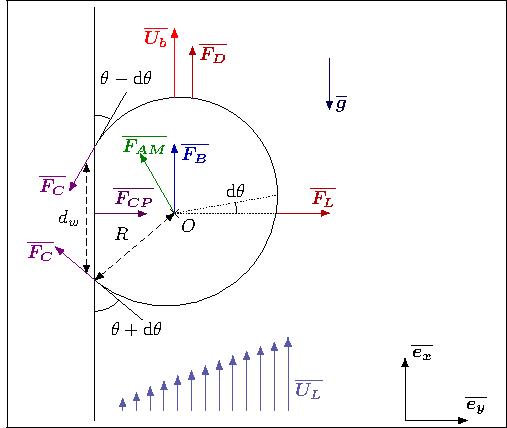
\includegraphics[width=0.6\linewidth]{img/bub_dyn/bub_bdf.pdf}
\caption{Sketch of the forces applied to the bubble facing an upward flow $\vect{U_{L}}$ and sliding at velocity $\vect{U_{b}}$}
\label{fig:bub_forces}
\end{figure}



Regarding the bubble shape, we consider a quasi-spherical bubble of radius $R$ with a circular contact area with the wall of radius $r_{w}$. It has a static contact angle $\theta$ and is tilted under the influence of the flow by an inclination angle $\dtheta$ (half the total angle hysteresis). The resulting downstream and upstream contact angles are therefore $\theta_{d}=\theta-\dtheta$ and $\theta_{u}=\theta+\dtheta$. If the bubble has a shape close to a truncated sphere, we can approximate the bubble foot radius as:

\begin{equation}
r_{w} \approx R~ \sin{\frac{\theta_{u}+\theta_{d}}{2}}=R~ \sin{\theta}
\label{eq:rw}
\end{equation}

Some authors rather take $r_{w}\approx \dfrac{1}{2} R~\parth{\sin{\theta_{u}} + \sin{\theta_{d}} }=R~\sin{\theta}\cos{\dtheta}$, however this expression tends to zero when reaching $\dtheta \to 90\degree$ which is undesirable regarding the expression of forces such as Contact Pressure and Surface Tension.


We suppose $V_{b}\approx\frac{4}{3}\pi R^{3}$ for the bubble volume.





\subsection{Buoyancy Force}


The buoyancy force results from both the weight of the bubble and the integration of the hydrostatic liquid pressure over its surface which naturally yields:
\begin{equation}
\vect{F_{B}}= \rho_{V}V_{b}\ \vect{g} + \parth{\iint_{S_{b}} \rho_{L} g z\ \mathrm{d}^{2}S}\vect{e_{x}} = V_{b}\parth{\rho_{V}-\rho_{L}}\vect{g}=\frac{4}{3}\pi R^{3}\parth{\rho_{L}-\rho_{V}}g \ \vect{e_{x}}
\label{eq:force_buoyancy}
\end{equation}

\subsection{Contact Pressure Force}

The contact pressure force arises due to the pressure difference between the center of the bubble and the surrounding liquid.  Combined with the Archimedes force, it can be expressed versus the difference of liquid and vapor pressure at the bubble foot using Laplace's equation $\Delta P = 2\sigma / R_{c}$ as:

\begin{align}
\vect{F_{CP}}  \approx \frac{2\sigma}{R_{c}} \pi r_{w}^{2}\  \vect{e_{y}}
\approx \pi R \sigma\ 2\ \sin{\theta}^{2}\ \vect{e_{y}}
\label{eq:FCP}
\end{align}

Here, $R_{c}$ is the curvature radius of the bubble which is often assumed to be equal to $5R$ \cite{klausner_vapor_1993, sugrue_modified_2016, mazzocco_reassessed_2018} without other explanation than avoiding an overestimation of the contact pressure force. To avoid this arbitrary choice, following the hypothesis of a nearly spherical bubble shape gives $R_{c}=R$.


\subsection{Capillary Force}

The capillary force acts at the triple contact line at the bubble's foot and is an important adhesive force maintaining the bubble attached to the wall. Its derivation can be done by integration of the effort exerted over the triple contact line. Noting $\Phi$ the polar angle around the bubble foot, we have :


\begin{equation}
\vect{F_{C}} = 2 \int_{0}^{\pi} \sigma r_{w} \vect{\tau}\parth{\Phi} \mathrm{d}\Phi
\end{equation}
where $\vect{\tau}$ is the unit vector tangent to the interface.

To compute the resulting components parallel and tangent to the wall, Klausner \etal \cite{klausner_vapor_1993} account for a contact angle difference between the upstream (receeding) contact angle $\theta_{u}$ and downstream (advancing) contact angle $\theta_{d}$. If the local contact angle is noted $\gamma$, then:

\begin{equation}
\vect{\tau}\parth{\Phi} = \cos{\gamma} \cos{\Phi} \vect{e_{x}} + \sin{\gamma} \vect{e_{y}}
\end{equation}

Then representing the evolution of the local contact angle $\gamma$ from $\theta_{u}$ to $\theta_{d}$ using a polynomial expression of degree 3:


\begin{equation}
\gamma\parth{\Phi} = \theta_{d} + \parth{\theta_{u} - \theta_{d}} \crocht{3\parth{\frac{\Phi}{ \pi}}^{2} - 2\parth{\frac{\Phi}{\pi}}^{3}},\ 0 \leq \Phi \leq \pi
\label{eq:forces_klausner_poly_deg3}
\end{equation}
which verifies symmetry conditions:

\begin{equation}
\gamma'\parth{0} = \theta_{d},\ \gamma\parth{\pi} = \theta_{u},\ \gamma'\parth{0}=\gamma'\parth{\pi}=0
\end{equation}

To obtain analytic expression, Klausner \etal also consider a first order linear interpolation:

\begin{equation}
\gamma\parth{\Phi} = \theta_{d} + \parth{\theta_{u}-\theta_{d}}\frac{\Phi}{\pi}
\end{equation}

This yields:

\begin{equation}
\vect{F_{C}}=-2r_{w}\sigma \frac{\pi\parth{\theta_{u}-\theta_{d}}}{\pi^{2}-\parth{\theta_{u}-\theta_{d}}^{2}}\parth{\sin{\theta_{u}}+\sin{\theta_{d}} }\vect{e_{x}} - 2r_{w} \sigma \frac{\pi}{\theta_{u}-\theta_{d}}\parth{\cos{\theta_{d}}- \cos{\theta_{u}}}\vect{e_{y}}
\label{eq:forces_FC_klausner_deg1}
\end{equation}

By comparing the analytic expression of Eq. \ref{eq:forces_FC_klausner_deg1} with the values obtained by numerical integration of Eq.\ref{eq:forces_klausner_poly_deg3}, Klausner \etal introduce a correction factor of $1.25$ over the $x$ component, finally giving :

\begin{align}
\vect{F_{C}}&=-2.5r_{w}\sigma \frac{\pi\parth{\theta_{u}-\theta_{d}}}{\pi^{2}-\parth{\theta_{u}-\theta_{d}}^{2}}\parth{\sin{\theta_{u}}+\sin{\theta_{d}} }\vect{e_{x}} - 2r_{w} \sigma \frac{\pi}{\theta_{u}-\theta_{d}}\parth{\cos{\theta_{d}}- \cos{\theta_{u}}}\vect{e_{y}}\\
%
&=-\pi R \sigma \underbrace{\crocht{2.5~ \frac{r_{w}}{R} \frac{\dtheta}{\parth{\frac{\pi}{2}}^{2}-\dtheta^{2}}\sin{\theta}\cos{\dtheta}}}_{f_{C,x}} \vect{e_{x}} - \pi R \sigma \underbrace{\crocht{2\ \frac{r_{w}}{R} \sin{\theta} \frac{\sin{\dtheta}}{\dtheta}}}_{f_{C,y}} \vect{e_{y}}
\label{eq:forces_FC}
\end{align}

\begin{remark*}{}
We can see that $f_{C,x} \to 0$ and $f_{C,y} \to 2\dfrac{r_{w}}{R}\sin{\theta}$  when $\dtheta \to 0$. In that case, $\vect{F_{C}} = -\vect{F_{CP}}$.
\end{remark*}





\subsection{Drag and Lift Forces}
\label{subsec:drag_lift}


The external liquid flow over the bubble induces the well-known drag and lift forces, acting respectively in the flow direction and perpendicular to the flow. They are usually expressed using associated coefficients $C_{D}$ and $C_{L}$ defined by:
\begin{align}
\vect{F_{D}}=&\frac{1}{2}C_{D}\rho_{L}S_{p} \norm{ \vect{U_{L}}-\vect{U_{b}} } \parth{\vect{U_{L}}-\vect{U_{b}}} \\
\vect{F_{L}}=&\frac{1}{2}C_{L}\rho_{L}S_{p}\norm{\vect{U_{L}}-\vect{U_{b}}}^{2}\ \vect{e_{y}}
\end{align}
with $S_{p}=\pi R^{2}$ the projected area of the bubble in the direction of the flow.

\subsubsection{Drag Coefficient}

Derivations of analytic expressions for the drag coefficient in an infinite fluid medium exist for more than a century, starting with Hadamard-Rybzinski (1911) \cite{hadamard_1911}:

\begin{equation}
C_{D} = \frac{16}{\Re_{b}},\ \text{if}\ \Re_{b}<1
\end{equation}
where $\Re_{b} = \frac{\bars{U_{rel}}D_{B}}{\nu_{L}}$ is the bubble Reynolds number and $U_{rel}$ the relative velocity between the bubble and the surrounding fluid.

For $\Re_{b} \gg 1$, Levich (1962) \cite{levich_1962} found for a potential flow:

\begin{equation}
C_{D} = \frac{48}{\Re_{b}}
\end{equation}


For intermediate values of $\Re_{b}$, traditional approaches rely on expressions of the drag force for a bubble in an infinite medium based on numerical correlations as proposed by Mei \& Klausner \cite{mei_unsteady_1992}, used in many different mechanistic approaches \cite{zeng_unified_1993-1, thorncroft_bubble_2001, chen_prediction_2012, sugrue_modified_2016, ren_development_2020}:

\begin{equation}
C_{D,U} = \frac{16}{\Re_{b}}\crocht{1 + \parth{\frac{8}{\Re_{b}}+ \frac{1}{2}\parth{1+\frac{3.315}{\sqrt{\Re_{b}}} }}^{-1} }
\label{eq:CD_mei}
\end{equation}


Results from DNS conducted by Legendre \etal \cite{legendre_lift_1998} proposed expressions of the drag and lift forces for a hemispherical bubble on a wall facing a viscous shear flow. Earlier, Legendre \& Magnaudet \cite{legendre_lift_1998} analytically derived coefficients to transpose drag and lift expressions for a particle to the case of a bubble. This was applied by Mazzocco \etal \cite{mazzocco_reassessed_2018} to the Drag for a solid particle near a wall in a shear flow proposed by Zeng \etal \cite{zeng_forces_2009}.

\npar

In this work, we propose to rely on the recent work of Shi \etal \cite{shi_drag_2021} who conducted DNS of a shear flow over a spherical bubble of constant radius close to a wall for bubble Reynolds number between $10^{-1}$ and $10^{3}$ and non-dimensional shear rates between -0.5 and 0.5. A sketch of the situation simulated by Shi \etal is depicted on Figure \ref{fig:shi_scheme}.

\begin{figure}[h!]
\centering
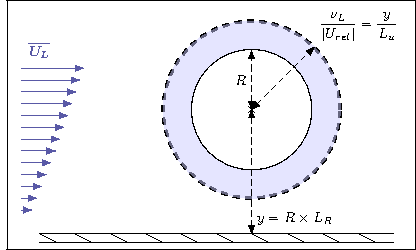
\includegraphics[width=0.55\linewidth]{img/bub_dyn/shi_scheme.pdf}
\caption{Physical situation considered by Shi \etal \cite{shi_drag_2021}.}
\label{fig:shi_scheme}
\end{figure}


They computed the resulting drag and lift coefficients for each simulations and proposed correlations fitting their numerical results. The total Drag coefficient is expressed as a correction of the Drag coefficient for a bubble in an unbounded uniform flow  $C_{D,U}$. The total drag is given by:

\begin{equation}
C_{D}=\parth{1+\Delta C_{D}}C_{D,U}
\end{equation}
where $\Delta C_{D}$ accounts for both the effect of the shear flow and the wall vicinity. 

\npar
To cover the whole range of bubble Reynolds numbers, correlations at low and high $\Re_{b}$ are smoothly connected using an exponential term.

\begin{equation}
\Delta C_{D}=\Delta C_{D,\Re_{b}=O\parth{1}}+\parth{1-e^{-0.07\Re_{b}}}\Delta C_{D,{\Re_{b}\gg 1}}
\label{eq:drag_corr_shi}
\end{equation}


Each of those corrections is computed depending on $\Re_{b}$,  the non-dimensional shear rate $\Sr = \dfrac{2 \gamma R}{\bars{U_{rel}} }$ where $\gamma = \dpartial{U_{L,x}}{y}$, the non dimensional wall distance $L_{R} = \dfrac{y}{R}$   ($L_{R}=1$ being a spherical bubble laying on a wall) and non-dimensional viscous (or Stokes) length $L_{u}=\dfrac{y}{\nu_{L}/\bars{U_{rel}}}$. 


\begin{align}
\nonumber \Delta C_{D,\Re_{b}=O\parth{1}} = & \frac{1+\mathrm{tanh}\parth{0.012\Re_{b}^{0.8}} + \mathrm{tanh}\parth{0.07\Re_{b}^{0.8}}^{2}}{1+0.16L_{u}\parth{L_{u}+4}}\\
& \times \left[ \left(\frac{3}{8}L_{R}^{-1} + \frac{3}{64}L_{R}^{-4}\right) \left(1- \frac{3}{8}L_{R}^{-1}-\frac{3}{64}L_{R}^{-4}\right)^{-1} - \frac{1}{16}\left(L_{R}^{-2}+\frac{3}{8}L_{R}^{-3}\right)\text{Sr} \right] \\
%
\nonumber\\
\Delta C_{D,{\Re_{b}\gg 1}} =& ~0.47L_{R}^{-4}+0.0055L_{R}^{-6}\Re_{b}^{3/4} 
+0.002 \bars{\mathrm{Sr}}^{1.9} \Re_{b} + 0.05 L_{R}^{-7/2} \mathrm{Sr} \Re_{b}^{1/3}
\end{align}


Figure \ref{fig:CD_shi} shows the evolution of the drag correction $\Delta C_{D}$ against the bubble Reynolds number for different distances to the wall $L_{R}$ and two values of $\Sr$.  We can see that as the distance between the wall and the bubble increases the drag correction logically approaches zero and that increasing the shear rate $\Sr$ increases $\Delta C_{D}$ for higher values of $\Re_{b}$.

\npar

Shi \etal \cite{shi_drag_2021} conducted DNS for wall distances down to $L_{R}=1.5$. However, Scheiff \etal \cite{scheiff_experimental_2021} compared the values obtained for $L_{R}=1$  with measured drag coefficients of bubbles sliding on a wall and observed a good agreement, which legitimates the use of this new drag correlation by extending its application to the case of a bubble laying on a wall and using the uniform drag coefficient of Eq.~\ref{eq:CD_mei}.


\begin{figure}[h!]
\centering
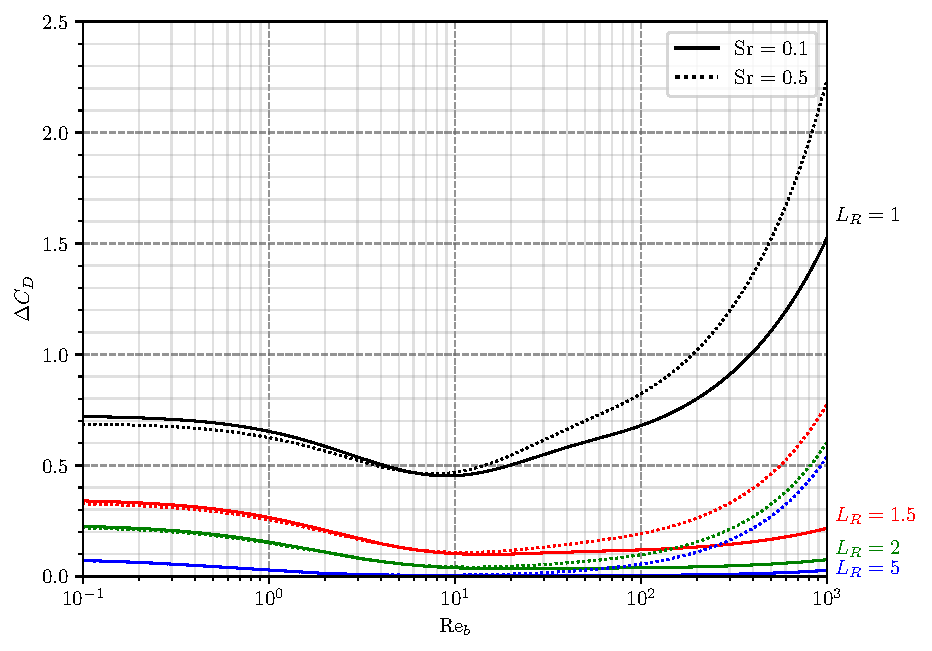
\includegraphics[width=0.6\linewidth]{img/bub_dyn/forces/corr_drag.pdf}
\caption{Drag correction from Shi \etal \cite{shi_drag_2021}.}
\label{fig:CD_shi}
\end{figure}


\begin{remark*}{}
In PWR conditions, a static bubble of radius $0.01$\ mm on a wall with a bulk liquid velocity of $5$\ m/s leads to a non-dimensional shear rate $\Sr \approx 0.7$ with $\Re_{b} \approx 500$. In this case, the drag correction can reach 180\% compared to the unbounded uniform flow formulation.
\end{remark*}


\subsubsection{Lift Coefficient}


In 1987, Auton \etal \cite{auton_1998} analytically derived the lift force for an inviscid fluid in unstationnary motion in a weak velocity gradient and found $C_{L}=0.5$, with the lift force defined as:

\begin{equation}
\vect{F_{L}} = - \rho_{L} C_{L} V_{b} \parth{\vect{U_{L}} - \vect{U_{b}}} \wedge \vect{\omega} 
\end{equation} 
where $\vect{\omega}$ is the flow vorticity.

\npar
This result was enriched by Legendre \& Magnaudet (1998) \cite{legendre_lift_1998bis} who used numerical results to propose a dependency of $C_{L}$ on the bubble Reynolds number for a sphere in an infinite medium facing a weakly sheared flows as:

\begin{align}
C_{L} =&\parth{ {C_{L,\Re_{b} \sim 1}}^{2} + {C_{L,\Re_{b} \gg 1}}^{2} }^{1/2}\\
 =&\parth{ \crocht{\frac{6}{\pi^{2}} \frac{2.255 \parth{\Re_{b}\omega^{*}}^{-1/2}}{ \parth{1+0.2\dfrac{\Re_{b}}{\omega^{*}}}^{3/2} }}^{2} + \crocht{ \frac{1}{2} \frac{1+16\ {\Re_{b}}^{-1}}{1+29\ {\Re_{b}}^{-1}} }^{2} }^{1/2}
\end{align} 
where $\omega^{*} = \dfrac{2R\bars{\vect{\omega}}}{\bars{U_{rel}}}$ is the non-dimensional vorticity of the flow.

\begin{remark*}{}
In the case of a steady linear shear flow near a wall, the vorticity is $\vect{\omega}=\overline{\nabla} \wedge \vect{U_{L}}=-\gamma\ \vect{e_{y}}$. In that case, the non-dimensional vorticity becomes the non-dimensional shear rate : $\omega^{*} = \dfrac{2R\gamma}{\bars{U_{rel}}} = \Sr$.
\end{remark*}


\npar

Later, Mei \& Klausner (1994) \cite{mei_klausner_lift} derived the lift force induced by the shear for a spherical bubble in an unbounded flow for low Reynolds numbers, based on the expression of Saffmann \cite{saffman_lift_particle}. By interpolating this result with the solution of Auton \cite{auton_lift_1987}, they obtained a formulation for a large range of $\Re_{b}$ :

\begin{equation}
C_{L} = 2.74 \sqrt{\Sr} \times \crocht{\Re_{b}^{-2} + \parth{0.24\sqrt{\Sr}}^{4}}^{1/4}
\label{eq:lift_mei}
\end{equation}

This expression is actually used in many mechanistic force balance \cite{klausner_vapor_1993, chen_prediction_2012, sugrue_modified_2016, ren_development_2020} \cite{chen_prediction_2012} \cite{ren_development_2020} 


\npar

In his force-balance approach, Mazzocco \etal \cite{mazzocco_reassessed_2018} used a constant lift coefficient by using the upper bound for the lift of a solid particle touching a wall in a Stokes flow, multiplied by $\dfrac{4}{9}$ to transpose this value to the bubble case as suggested by Legendre \& Magnaudet \cite{legendre_lift_1997_coeff}. This resulted in:

\begin{equation}
C_{L} = 2.61
\end{equation}


\npar

In accordance with the computation of the drag coefficient, our model will rely on the expression of the lift coefficient proposed by Shi \etal \cite{shi_drag_2021}. Their formulation includes extra parameters compared to the drag coefficient :
\begin{itemize}
\item The non-dimensional Saffman length $L_{\omega} = \dfrac{y}{\sqrt{\nu_{L} / \omega}}$ ;
\item The Stokes (or Oseen) length to Saffman length ratio $\varepsilon = \dfrac{\nu_{L} / \bars{U_{rel}}}{\sqrt{\nu_{L} / \omega}}$, which quantifies the origin of inertial effects being either shear ($\varepsilon >1$) or the relative slip of the bubble ($\varepsilon < 1$).

\end{itemize}  

The resulting formulation of $C_{L}$ corresponds to the superpositions of two contributions respectively associated to the uniform flow and the shear rate, both coupled with the wall presence. 

\begin{align}
C_{L}^{W} =C_{Lu}^{W} + C_{L\omega}^{W}
\label{eq:lift_shi}
\end{align}



The lift associated to the uniform flow near a wall is computed as follows:
\begin{align}
\nonumber C_{Lu}^{W} =&\  e^{-0.22\ \varepsilon^{0.8}L_{\omega}^{2.5}} \frac{ \crocht{1 + \tanh{0.012\ {\Re_{b}}^{0.8}} + \tanh{0.07\ {\Re_{b}}^{0.8}} }^{2} } {1+0.13\ L_{u} \parth{L_{u}+0.53} } \\
%
\nonumber			&\times  \parth{\frac{L_{R}}{3}}^{-2.0\ \tanh{0.01\Re_{b}}}  C_{Lu}^{\text{W-in}}\\
%
&+\parth{1-e^{-0.22\ {\Re_{b}}^{0.6}} } \crocht{ C_{Lu,\Re_{b}\to \infty}^{W} + 15\ \tanh{ 0.01\ \Re_{b} }{\Re_{b}}^{-1} L_{R}^{-4} }
%
\end{align}
Where:
\begin{align}
C_{Lu}^{\text{W-in}}=&\frac{1}{2}\left(1+\frac{1}{8}L_{R}^{-1}-\frac{33}{64}L_{R}^{-2}\right)\\
%
C_{Lu, \Re_{b} \to \infty}^{W} = & -\frac{3}{8}L_{R}^{-4}\left[1+\frac{1}{8}L_{R}^{-3}+\frac{1}{6}L_{R}^{-5}\right] + O\left(L_{R}^{-10}\right)
\end{align}


\npar

The lift associated to the vorticity near a wall is computed as follows:

\begin{align}
C_{L\omega}^{W} =& \crocht{ 1-\exp{ -\frac{11}{96}\pi^{2}\frac{L_{\omega}}{J_{L}(\varepsilon)} \parth{1+\frac{9}{8}L_{R}^{-1}-\frac{1271}{3520}L_{R}^{-2}} } }C_{L\omega, \Re_{b} \ll 1}^{U}\\
%
 & + \parth{1-e^{-0.3\ \Re_{b}} } \crocht{1+0.23\ L_{R}^{-7/2} \parth{1+13\ {\Re_{b}}^{-1/2}}} C_{L\omega, \Re_{b} \gg 1}^{U}
\end{align}

Where:

\begin{align}
J_{L}(\varepsilon)&=2.254 \parth{1+0.2\varepsilon^{-2}}^{-3/2} \\
%
C_{L\omega, \Re_{b} \ll 1}^{U} &= \frac{8}{\pi^{2}} \frac{\Sr}{\bars{\Sr}}\varepsilon J_{L}(\varepsilon)\\
%
C_{L\omega, \Re_{b} \gg 1}^{U}&= \frac{2}{3}\Sr \parth{ 1-0.07\bars{\Sr} }\frac{1+16\Re_{b}^{-1}}{1+29\Re_{b}^{-1}}
\end{align}


On Figure \ref{fig:lift_shi}, we plot the values of $C_{L}$ obtained by the formulation of Shi \etal different values of the non-dimensional wall distance $L_{R}$ (extending down to $L_{R}=1$) and non-dimensional shear rate $\Sr$.

\begin{figure}[h!]

\subfloat[Positive values of $\Sr$]{
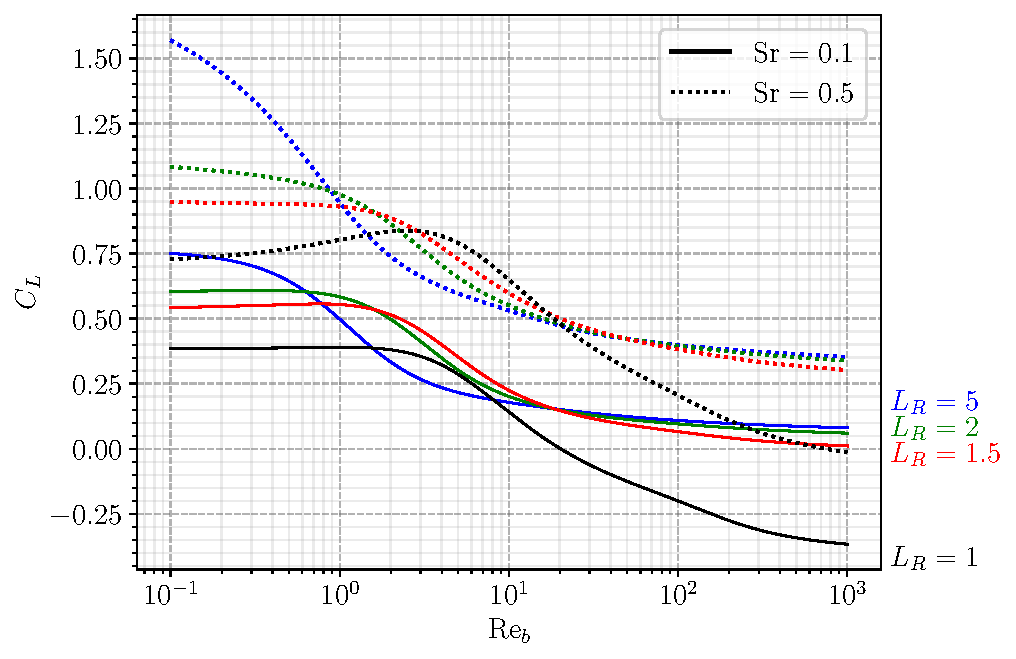
\includegraphics[width=0.5\linewidth]{img/bub_dyn/forces/lift_shi_srpos.pdf}
}
\subfloat[Negative values of $\Sr$]{
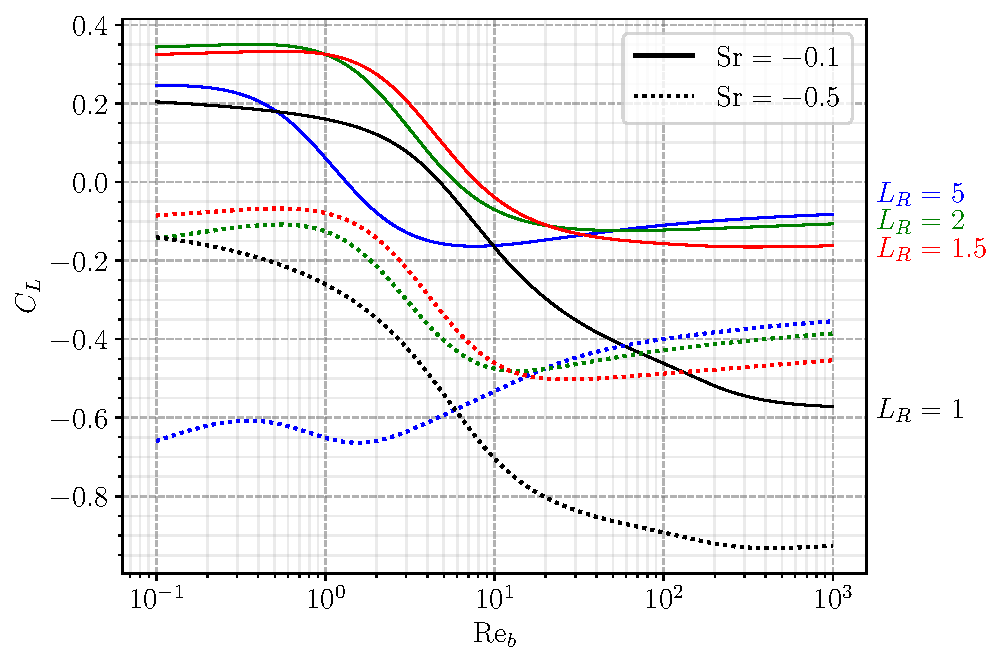
\includegraphics[width=0.5\linewidth]{img/bub_dyn/forces/lift_shi_srneg.pdf}
}

\caption{$C_{L}$ computed using Shi \etal correlation.}
\label{fig:lift_shi}
\end{figure}

We can see that the magnitude of the lift coefficient globally increases with the wall distance when $\Sr >0$ and that negative lift values are easily reached when $\Sr <0$. This means that correlations for unbounded medium may overestimate the lift experienced by the bubble compared to the situation with a wall. 

The extension to the case $L_{R}=1$ may be more questionable compared to the drag since the bubble touching the wall will stop any flow in between, leading to inertial and shear regimes that would be significantly different due to the redirection of the liquid at the bubble's foot towards the bulk. In particular, we can see that the values reached for $L_{R}=1$ on Figure \ref{fig:lift_shi} are not following the general trend of simulated $L_{R}$ :

\begin{itemize}
\item Negative values of $C_{L}$ are reached with positive $\Sr$ at high $\Re_{b}$ while getting close to the wall seemed to tend to a value of $C_{L} \geq 0$ at high $\Re_{b}$ ;
\item Magnitude of $C_{L}$ with negative $\Sr$ are not coherent with the observed trend down to $L_{R}=1.5$.
\end{itemize}

This observation suggest that we should include the effect of the wall using the lift of Shi \etal by limiting its use to $L_{R}=1.5$ contrary to the drag which extension to $L_{R}=1.0$ was coherent and validated.

\npar

\begin{remark*}{}
In PWR conditions, taking $\Sr \approx 0.7$ with $\Re_{b} \approx 500$ for the static bubble on a wall leads to $C_{L}\approx 0.45$ both with Mei \& Klausner (Eq. \ref{eq:lift_mei}) and Shi \etal (Eq. \ref{eq:lift_shi}). For a bubble that would slide at 90\% of the local liquid velocity, this gives $\Sr \approx 7$ and $\Re_{b} \approx 50$ yielding $C_{L,Mei} \approx 4$ and $C_{L,Shi} \approx 2.8$.
\end{remark*}


\subsection{Inertia Force}
\label{subsec:AM}

The Inertia force originates from various effects (bubble growth, freestream and bubble acceleration, etc.) and includes both added mass and Tchen forces and is expressed as presented in Magnaudet \& Eames (2000) \cite{magnaudet_motion_2000}:

\begin{equation}
\vect{F_{I}} = \underbrace{ \rho_{L}V_{b}\parth{\dtime{\vect{U_{L}}}+\vecgrad{\vect{U_{L}} }\cdot \vect{U_{L}}} }_{\text{Liquid inertia or Tchen force}} + \underbrace{ \derive{}{t}\parth{\rho_{L}C_{AM}V_{b}\parth{\vect{U_{L}}-\vect{U_{b}}}} }_{\text{Added Mass force } \vect{F_{AM}}}
\label{eq:F_inertia}
\end{equation}

Since we consider a steady and quasi-parallel liquid flow, we respectively have:

\begin{equation}
\dpartial{\vect{U_{L}} }{t}=0\ \text{and}\ \vecgrad{\vect{U_{L}} } cdot \vect{U_{L}}=0
\end{equation}

Thus only remains the added mass force to express in the considered force balance. In the next subsections, we detail former approaches to tackle the added mass derivation and propose a more rigorous to re-evaluate the added mass coefficients.


\subsubsection{Former Approaches}
\label{subsubsec:former_AM}

In previous mechanistic models, the derivation of the added mass force was conducted with different approaches. In particular, some authors chose to rely on the Rayleigh-Plesset Equation (RPE) for a growing hemispherical bubble in a quiescent flow to obtain the reaction force from the liquid, oriented perpendicularly to the wall:

\begin{equation}
\vect{F_{AM,RPE}}=- \rho_{L}\pi R^{2}\crocht{R\ddot{R}+\frac{3}{2}\dot{R}^{2}}\vect{e_{y}}
\end{equation}

Then, assuming a bubble inclination angle $\theta_{i}$, this force was projected along the $x$ axis to obtain an Added Mass force parallel to the wall that hinders departure. The inclination angle value is often empiricial and used for data fitting \cite{zeng_unified_1993-1, colombo_prediction_2015, mazzocco_reassessed_2018, ren_development_2020}.

\begin{equation}
\vect{F_{AM,RPE}}=- \rho_{L}\pi R^{2}\crocht{R\ddot{R}+\frac{3}{2}\dot{R}^{2}}\parth{\sin{\theta_{i}}\vect{e_{x}} + \cos{\theta_{i}}\vect{e_{y}}}
\label{eq:AM_RPE}
\end{equation}


This approach is questionable on different aspects. First, the RPE assumes a moving boundary in a quiescent unbounded liquid, which is physically far from the real situation of a bubble growing on a wall in a boiling flow. Moreover, the subsequent projection along the different directions regarding an unknown angle is hardly reasonable if $\theta_{i}$ is chosen arbitrarily. Values of $\theta_{i}$ selected by different authors are mentioned in Table \ref{tab:all_BdF}.

\npar

On the other hand, some authors \cite{klausner_vapor_1993, thorncroft_bubble_2001, guan_bubble_2015} considered two distinct contributions: 

\begin{itemize}

\item Hemispherical bubble growth in a stagnant liquid, leading to Eq.~\ref{eq:AM_RPE} including the inclination angle $\theta_{i}$ ;
\item Spherical bubble growth in an uniform unbounded and inviscid liquid flow, which yields a detaching Added Mass term  due to the interaction of bubble growth with the external flow: 
\begin{equation}
\vect{F_{AM,U}}= \frac{3}{2}\rho_{L}V_{b}\frac{\dot{R}}{R}U_{L} \vect{e_{x}} 
\label{eq:AM_bulk}
\end{equation} 

\end{itemize}

This last term is usually called a "bulk growth force". By including the effect of the liquid flow, this approach can be considered as closer to the reality. However, it relies on two separate derivations associated to different physical considerations.



\subsubsection{Proposed Approach}
\label{subsubsec:new_AM}

To tackle the added mass derivation in a proper way, we propose to follow the approach of Lamb \cite{lamb_hydrodynamics_1895} (also presented by Milne Thomson \cite{milne-thomson_theoretical_1938} or Van Winjgaarden \cite{wijngaarden_hydrodynamic_1976}). By solving the potential flow around a bubble and its image, we can obtain the total liquid kinetic energy $E_{L}$ that corresponds to a situation where a bubble is at a given distance from a wall (represented by the line normal to the line of centers of the bubbles). 

Then we can use Lagrange equation to compute the resulting forces along a given coordinate $q$:


\begin{align}
\label{eq:Lag_x}
F_{AM,q}&=-\dpartial{}{t}\parth{\dpartial{E_{L}}{\dot{q}}}+\dpartial{E_{L}}{q}\\
\end{align}


This method was also used by Duhar \cite{duhar_dynamics_2006} who developed an asymptotic expression of $E_{L}$ to compute the addd mass coefficient when the bubble approaches the wall. Here, we express the liquid kinetic energy by relying on the work of Van Der Geld \cite{van_der_geld_dynamics_2009} who derived $E_{L}$ in the case of a full or truncated spherical bubble laying on a wall and facing an uniform flow parallel to the wall of velocity $U_{L}$ (Eq.~\ref{eq:EL_VdG}). If the bubble slides at a velocity $U_{b}=\dot{x}$, it sees a liquid velocity $U_{rel}=U_{L}-\dot{x}$.

\begin{align}
E_{L}=\frac{\rho_{L}V_{b}}{2}\parth{\alpha \dot{y}^{2} +\trb\dot{R}^{2}+\psi \dot{R}\dot{y} +\alpha_{2} \parth{U_{L}-\dot{x}}^{2} }
\label{eq:EL_VdG}
\end{align}
where $(x,y)$ are the coordinates of the bubble's center and $\alpha$, $\trb$, $\psi$, $\alpha_{2}$ are polynomials of $R/y = 1/L_{R}$ derived by Van Der Geld for $1<R/y<2$ \ie $0.5<L_{R}<1$, corresponding to contact angles $0\degree < \theta \ 60\degree$.

\npar
For each polynomial expression ($\alpha$ is used as an example), we note $n$ its degree and write:

\begin{equation}
\alpha = \sum_{k=0}^{n}\alpha_{k}\parth{\frac{R}{y} }^{k}\ \text{and}\ \tilde{\alpha}= \sum_{k=0}^{n}k\ \alpha_{k}\parth{\frac{R}{y} }^{k}
\end{equation}

This allows to express the following derivatives:

\begin{equation}
\dpartial{\alpha}{y} = -\frac{1}{y} \tilde{\alpha}\ \text{and}\ \dpartial{\alpha}{t} = \parth{\frac{\dot{R}}{R} - \frac{\dot{y}}{y}} \tilde{\alpha}
\end{equation}


Noticing that the derivatives of the polynomials along $x$ will be 0 and injecting $E_{L}$ in Eq.~\ref{eq:Lag_x} and \ref{eq:Lag_y} allows to express the added mass force in $x$ and $y$ directions. If we express it using geometrical ratios $\dfrac{R}{y}=\dfrac{1}{F_{1}}$, $\dfrac{\dot{y}}{\dot{R}}=F_{2}$ and $\dfrac{\ddot{y}}{\ddot{R}}=F_{3}$, we can obtain:

\begin{align}
F_{AM,x} = \rho_{L}V_{b} \crocht{ \parth{ 3\alpha_{2} +\parth{1-\frac{F_{2}}{F_{1}}}\tilde{\alpha_{2}} } \frac{\dot{R}}{R}U_{rel} - \alpha_{2} \dtime{U_{b}} }
\end{align}

\begin{align}
\nonumber F_{AM,y} = - \rho_{L} V_{b} & \left[ \parth{ 3 F_{2}\alpha + \frac{3}{2}\psi + \parth{1- \frac{F_{2}}{F_{1}}}F_{2} \tilde{\alpha} + \parth{1- \frac{F_{2}}{F_{1}}}\frac{\tilde{\psi}}{2}  + \frac{F_{2}}{F_{1}}\frac{\tilde{\alpha}}{2} + \frac{1}{F_{1}} \frac{\tilde{\trb}}{2} + \frac{F_{2}}{F_{1}} \frac{\tilde{\psi}}{2}}\frac{\dot{R}^{2}}{R} \right.\\
& \left.  + \parth{F_{3}\alpha + \frac{\psi}{2}}\ddot{R} + \frac{1}{F_{1}}\frac{\tilde{\alpha_{2}}}{2} \frac{U_{rel}^{2}}{R}  \right] 
\end{align}


In the case of a truncated sphere, $F_{1} = \dfrac{y}{R} = \cos{\theta}=L_{R}$. If we suppose that the bubble keeps a nearly constant contact angle during its lifetime, we can further write $F_{1}=F_{2}=F_{3}=\cos{\theta}=L_{R}$, which simplifies the forces in:


\begin{align}
F_{AM,x} = \rho_{L}V_{b} \crocht{ 3\alpha_{2} \frac{\dot{R}}{R}U_{rel} - \underbrace{\alpha_{2}}_{C_{AM,x}} \dtime{U_{b}} }
\label{eq:FAMx}
\end{align}


\begin{align}
F_{AM,y} = \rho_{L} V_{b} & \left[  -\parth{ 3 \underbrace{\parth{L_{R}\alpha + \frac{\psi}{2} } }_{C_{AM,y1}} + \underbrace {\frac{\tilde{\alpha}}{2} + \frac{1}{L_{R}} \frac{\tilde{\trb}}{2} + \frac{\tilde{\psi}}{2}}_{C_{AM,y2}} } \frac{\dot{R}^{2}}{R} \right. \\
%
& \left. - \underbrace{ \parth{L_{R}\alpha + \frac{\psi}{2}} }_{C_{AM,y1}} \ddot{R} + \underbrace{ \frac{-1}{L_{R}}\frac{\tilde{\alpha_{2}}}{2} }_{C_{AM,y3}} \frac{U_{rel}^{2}}{R}  \right] 
\label{eq:FAMy}
\end{align}


On Figure \ref{fig:AM_coeff}, we plot the values of the added mass coefficients against the values of $L_{R}$. 

\begin{figure}[h!]
\centering
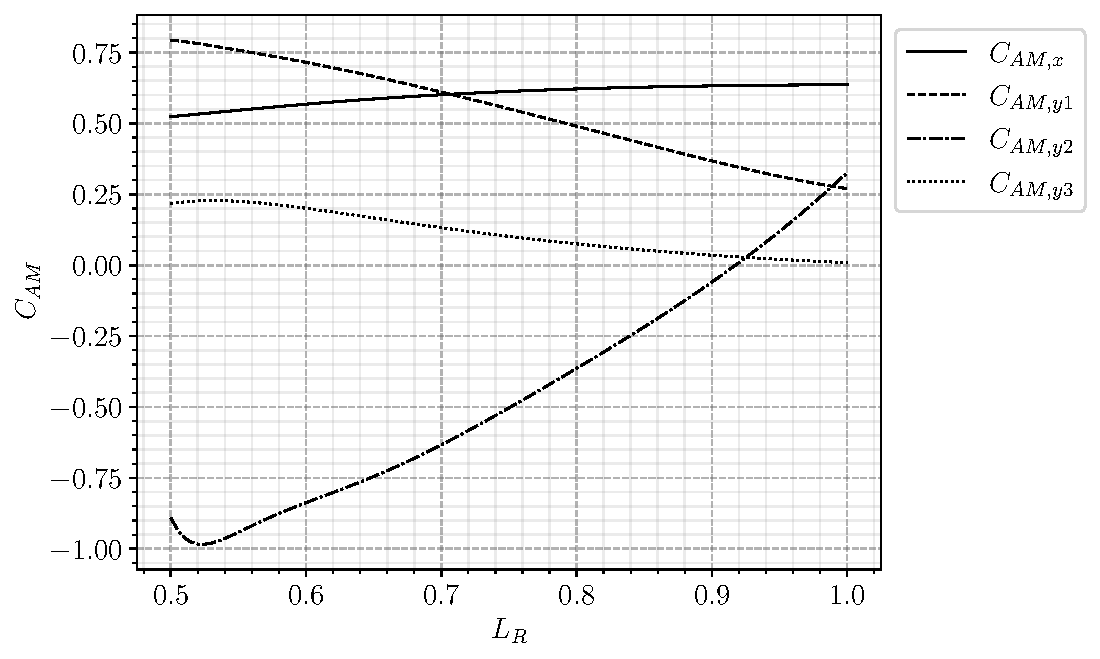
\includegraphics[width=0.65\linewidth]{img/bub_dyn/forces/CAM_plot.pdf}
\caption{Values of the computed added mass coefficients in Eq. \ref{eq:FAMx} and \ref{eq:FAMy}. }
\label{fig:AM_coeff}
\end{figure}

For the case of a spherical bubble laying on a wall ($L_{R}=1$), we finally have:



\begin{align}
F_{AM,x}=\rho_{L}V_{b}\crocht{3C_{AM,x}\frac{\dot{R}}{R}U_{rel} - C_{AM,x}\dtime{U_{b}}}
\label{eq:AMx}
\end{align}
with $C_{AM,x} \approx 0.636$.


\begin{align}
F_{AM,y}=\rho_{L}V_{b}\crocht{-\parth{3 C_{AM,y1} + C_{AM,y2}}\frac{\dot{R}^{2}}{R}-C_{AM,y1}\ddot{R} + C_{AM,y3}\frac{U_{rel}^{2}}{R}}
\label{eq:AMy}
\end{align}
with $C_{AM,y1} \approx 0.27$, $C_{AM,y2}\approx 0.326$ and $C_{AM,y3}\approx 8.77\times  10^{-3}$.


\npar

Parallel to the wall, the coupled term $\frac{\dot{R}}{R}U_{rel}$ in Eq.~\ref{eq:AMx} promotes detachment and sliding of the bubble if $U_{rel}>0$ \eg if the bubble is attached to its nucleation site. This contradicts the aforementioned approach where solely projecting the RPE on both axes lead to an Added-Mass term related to bubble growth that only hinders the departure by sliding. Moreover, Eq.~\ref{eq:AMy} exhibits a term induced by the relative velocity that acts as a lift force, which seems to rarely appear in other approaches.

\begin{remark*}{}
The derived values of the added mass coefficients are only valid for $0.5 < L_{R} < 1$ as previously mentioned. When the bubble leaves the wall, added mass calculations of Duhar \cite{duhar_phd} would be more appropriate.
\end{remark*}



\npar
Those theoretical results highlight the importance of conducting a rigorous approach when possible to deriving those transient aspects of the force balance. Otherwise, some terms may be missing and lead to contradictory physical conclusions. 

In the spirit of avoiding to introduce extra empirical terms, we keep the Added Mass force as presented in Eq.~\ref{eq:AMx} and \ref{eq:AMy} and consider no projection along the inclination angle.



\subsection{Force Balance Summary}\label{subsec:BdF}


Writing Newton's second law, we have the total force balance over the bubble in both directions:

\begin{align}
\nonumber \rho_{V} \dtime{V_{b}U_{b,x}} = & -\pi R \sigma f_{C,x}\parth{\theta, \dtheta} + V_{b}\parth{\rho_{L}-\rho_{V}}g + \frac{1}{2}C_{D}\rho_{L}\pi R^{2} \bars{U_{L}-U_{b}}\parth{U_{L}-U_{b}}\\
%
& + \rho_{L}V_{b}\crocht{3C_{AM,x}\frac{\dot{R}}{R}\parth{U_{L}-U_{b}} - C_{AM,x} \dtime{U_{b}}}
\label{eq:bdf_x}
\end{align}

\begin{align}
\nonumber \rho_{V} \dtime{V_{b}U_{b,y}} = & -\pi R \sigma f_{C,y}\parth{\theta, \dtheta} + 2\pi R \sigma \sin{\theta}^{2} + \frac{1}{2}C_{L}\rho_{L}\pi R^{2} \parth{U_{L}-U_{b}}^{2}\\
%
& + \rho_{L}V_{b}\crocht{-\parth{3 C_{AM,y1} + C_{AM,y2}}\frac{\dot{R}^{2}}{R}-C_{AM,y1}\ddot{R} + C_{AM,y3}\frac{\parth{U_{L}-U_{b}}^{2}}{R}}
\label{eq:bdf_y}
\end{align}

Those force balances will respectively be used later to study the departure by sliding (along $x$) and the lift-off from the wall (along $y$).

\npar

On Table \ref{tab:all_BdF}, we sum up some of the mentioned mechanistc approaches and their models along with the proposed force balance.



\begin{table}[h!]



\scriptsize
\centering

\noindent\makebox[\textwidth]{
\renewcommand{\arraystretch}{2.0}


\begin{tabular}{p{2mm} p{6mm}|p{50mm}|p{50mm}|p{50mm}}

 & & Klausner (1993) \cite{klausner_vapor_1993} & Thorncroft (2001) \cite{thorncroft_bubble_2001} & Sugrue (2016) \cite{sugrue_modified_2016} \\
\hline

\multirow{6}*{\rotatebox{90}{Forces}} &  $\vect{F_{B}}$ & $\frac{4}{3}\pi R^{3} \parth{\rho_{L}-\rho_{V}}\vect{g}$ & $\frac{4}{3}\pi R^{3}\parth{\rho_{L}-\rho_{V}}\vect{g}$ & $\frac{4}{3}\pi R^{3}\parth{\rho_{L}-\rho_{V}}\vect{g}$ \\

& $\vect{F_{C}}$ & Eq. \ref{eq:FC_klausner}, $r_{w}=0.045$ mm & Eq. \ref{eq:FC_klausner}, $r_{w}=R~\sin{\theta_{d}}$ & Eq. \ref{eq:FC_klausner}, $r_{w}=0.025R$ \\

& $\vect{F_{CP}}$ &  Eq.~\ref{eq:FCP}, $R_{c}=5R$ &  Neglected &  Eq.~\ref{eq:FCP}, $R_{c}=5R$  \\

& \multirow{2}*{$\vect{F_{D}}$} & $C_{D}=\frac{16}{\Re_{b}} \left[ 1+\frac{3}{2} \left( \parth{\frac{12}{\Re_{b}}}^{n}\right. \right.$\newline$ \left. \left. \quad \quad + 0.796^{n} \right) ^{1/n} \right]$, $n=0.65$ & $C_{D} = \frac{16}{\Re_{b}} \left[ 1 + \left(\frac{8}{\Re_{b}} \right. \right.$\newline$\left. \left. \quad  \quad + \frac{1}{2}\parth{1+\frac{3.315}{\sqrt{\Re_{b}}} } \right)^{-1} \right]$ & $C_{D}=\frac{16}{\Re_{b}} \left[ 1+\frac{3}{2} \left( \parth{\frac{12}{\Re_{b}}}^{n}\right. \right.$\newline$ \left. \left. \quad \quad + 0.796^{n} \right) ^{1/n} \right]$, $n=0.65$ \\

& \multirow{2}*{$\vect{F_{L}}$} & $C_{L}=2.74\sqrt{\Sr}$\newline$\times\crocht{\Re_{b}^{-2} + \parth{0.24\sqrt{\Sr}}^{4} }^{\frac{1}{4}}$ & $C_{L}=0.71\sqrt{\Sr}$\newline$\times\crocht{\parth{\frac{1.15\mathrm{J}(\varepsilon)}{\sqrt{\Re_{b}}}}^{2} + \parth{\frac{3\sqrt{2\Sr}}{8}}^{2} }^{\frac{1}{2}}$ & $C_{L}=2.74\sqrt{\Sr}$\newline$\times\crocht{\Re_{b}^{-2} + \parth{0.24\sqrt{\Sr}}^{4} }^{\frac{1}{4}}$   \\

& \multirow{2}*{$\vect{F_{AM}}$} & {$\frac{3}{2}\rho_{L}V_{b}\frac{\dot{R}}{R}U_{L} \vect{e_{x}}$ {$-\rho_{L}\pi R^{2}\parth{\frac{3}{2}\dot{R}^{2} + R\ddot{R}}$\newline$\times \parth{\cos{\theta_{i}}\vect{e_{y}} + \sin{\theta_{i}}\vect{e_{x}}}$, $\theta_{i}=10\degree$ }} & {$2\pi \rho_{L}R^{2}\dot{R}U_{L}\vect{e_{x}}$} {$-\rho_{L}\pi R^{2}\parth{\frac{3}{2}\dot{R}^{2} + R\ddot{R}}$\newline$\times \parth{\cos{\theta_{i}}\vect{e_{y}} + \sin{\theta_{i}}\vect{e_{x}}}$, $\theta_{i}=45\degree$ } & {{$-\rho_{L}\pi R^{2}\parth{\frac{3}{2}\dot{R}^{2} + R\ddot{R}}$\newline$\times \parth{\cos{\theta_{i}}\vect{e_{y}} + \sin{\theta_{i}}\vect{e_{x}}}$, $\theta_{i}=10\degree$ }} \\
\hline
\end{tabular}
}

\npar

\noindent\makebox[\textwidth]{
\renewcommand{\arraystretch}{2.0}

\begin{tabular}{p{2mm} p{6mm}|p{50mm}|p{50mm}|p{50mm}}
 & & Mazzocco (2018) \cite{mazzocco_reassessed_2018} & Ren (2020) \cite{ren_development_2020} & Present model \\
\hline

\multirow{6}*{\rotatebox{90}{Forces}} &  $\vect{F_{B}}$ & $\frac{4}{3}\pi R^{3} \parth{\rho_{L}-\rho_{V}}\vect{g}$ & $\frac{4}{3}\pi R^{3} \parth{\rho_{L}-\rho_{V}}\vect{g}$ & $\frac{4}{3}\pi R^{3} \parth{\rho_{L}-\rho_{V}}\vect{g}$ \\

& $\vect{F_{C}}$ & Eq. \ref{eq:FC_klausner}, $r_{w}=R/15$ & Eq. \ref{eq:FC_klausner}, $r_{w}=0.2R$& Eq. \ref{eq:FC_klausner}, $r_{w}=R\ \sin{\theta}$ \\

& $\vect{F_{CP}}$ & Eq.~\ref{eq:FCP}, $R_{c}=5R$ &  Eq.~\ref{eq:FCP}, $R_{c}=5R$ &  Eq.~\ref{eq:FCP}, $R_{c}=R$   \\

& \multirow{2}*{$\vect{F_{D}}$} & \multirow{2}*{$C_{D}=1.13\frac{24}{\Re_{b}}\parth{1+0.104\Re_{b}^{0.753}}$} & $C_{D}=\frac{16}{\Re_{b}} \left[ 1+\frac{3}{2} \left( \parth{\frac{12}{\Re_{b}}}^{n}\right. \right.$\newline$ \left. \left. \quad \quad + 0.796^{n} \right) ^{1/n} \right]$, $n=0.65$ & $C_{D}=C_{D,U}\parth{1+\Delta C_{D}}$ \newline $C_{D,U}$ by Eq. \ref{eq:CD_mei}, $\Delta C_{D}$ by Eq. \ref{eq:drag_corr_shi} \\

& \multirow{2}*{$\vect{F_{L}}$} & \multirow{2}*{$C_{L}=2.61$} & $C_{L}=2.74\sqrt{\Sr}$\newline$\times\crocht{\Re_{b}^{-2} + \parth{0.24\sqrt{\Sr}}^{4} }^{\frac{1}{4}}$ & \multirow{2}*{$C_{L}$ by Shi \etal \cite{shi_drag_2021}}   \\

& \multirow{2}*{$\vect{F_{AM}}$} & {$-\frac{1}{4}\pi \rho_{L} K^{4}\parth{\cos{\theta_{i}}\vect{e_{y}} + \sin{\theta_{i}}\vect{e_{x}}}$, $\sin{\theta_{i}}=0.2$, $\cos{\theta_{i}}=1$} & {$-\rho_{L}\pi R^{2}\parth{\frac{3}{2}\dot{R}^{2} + R\ddot{R}}$\newline$\times \parth{\cos{\theta_{i}}\vect{e_{y}} + \sin{\theta_{i}}\vect{e_{x}}}$, $\theta_{i}=15\degree$ } & {$\frac{F_{AM,x}}{\rho_{L}V_{b}}=C_{AM,x}\crocht{3\frac{\dot{R}}{R}U_{rel} - \dtime{U_{b}}}$, $C_{AM,x}=0.636$, $F_{AM,y}$ by Eq. \ref{eq:AMy}.} \\
\hline
\end{tabular}

}


\caption{Summary of different force-balance mechanistic approaches.}
\label{tab:all_BdF}
\end{table}


\subsection{Liquid Velocity}\label{subsec:liq_vel}

To compute the liquid velocity and shear rate at bubble center height, we use the wall law of Reichardt \cite{reichardt_vollstandige_1951}, which describes the velocity profile from the viscous sublayer to the logarithmic region.

\begin{align}
U_{L}^{+} =& \frac{1}{\kappa}\ln{1+\kappa y^{+}} + c \parth{1-e^{-y^{+}/\chi} + \frac{y^{+}}{\chi}e^{-y^{+}/3} }\\
%
\nonumber U_{L}=&U_{L}^{+}U_{\tau}
\end{align}
with $\kappa = 0.41$, $\chi = 11$ and $c=7.8$.

\begin{align}
\dpartial{U_{L}^{+}}{y^{+}} =& \frac{1}{1+\kappa y^{+}}+\frac{c}{\chi}\parth{e^{-y^{+}/\chi} + \parth{1-\frac{y^{+}}{3}}e^{-y^{+}/3}}\\
%
\nonumber \dpartial{U_{L}}{y} =& \gamma = \frac{U_{\tau}^{2}}{\nu_{L}} \dpartial{U_{L}^{+}}{y^{+}}
\end{align}

The friction velocity is computed using Mac Adams correlation \cite{mcadams_heat_1954}.

\begin{align}
U_{\tau} =& \sqrt{\frac{\tau_{w}}{\nu_{L}}}\\
\tau_{w} =& 0.018~ \Re_{D_{h}}^{-0.182}~ \frac{G_{L}^{2}}{\rho_{L}}
\end{align}

\newpage


\section{Bubble Growth}
\label{sec:bub_growth}

\subsection{Introduction}

In order to properly represent the bubble dynamics, it is mandatory to model the evolution of the bubble radius over time \ie the bubble growth law. Since the bubble radius $R$ and its derivatives $\dot{R}$ and $\ddot{R}$ appear in the force balance (notably in the expression of the added mass force \ref{eq:FAMy}), failing to predict the evolution of the bubble with time will definitely result in an erroneous force balance.

\npar
The problem of the bubble growth during its lifetime on the wall, including the sliding phase, is still an open question that aims to cover various types of heat transfer mechanisms. First, two growth regimes exist for a boiling bubble:

\begin{itemize}
\item Inertial growth, which occurs at the beginning of nucleation for low temperature difference between liquid and vapor. The evolution of the bubble size can be solved by the mass and momentum balances, through the solution of Rayleigh (1917) \cite{rayleigh_1917}. The form of the bubble growth is usually $R\parth{t} = A\times t$ (Mikic \& Rohsenow, \cite{mikic_1969}).

\item Heat diffusion growth happening post the inertial phase. This type of bubble growth has been widely studied by different authors \cite{plesset_growth_1954, scriven_dynamics_1959, zuber_dynamics_1961, mikic_1969} and is usually of the form $R\parth{t} = B\sqrt{t}$, derivable using the energy balance around the bubble.
\end{itemize}


Those two regimes can be compared using the non-dimensional time $t^{+}$ defined as:

\begin{align}
t^{+} = \frac{A^{2}}{B^{2}}t
\end{align}
where
\begin{equation}
A=\sqrt{b \frac{h_{LV}\rho_{V}\parth{T_{L}-T_{V}}}{\rho_{L}T_{sat}} } \ \text{and}\ B=\sqrt{\frac{12}{\pi}\eta_{L}}\Ja
\end{equation}
with $b=\dfrac{2}{3}$ for a bubble in an infinite liquid medium and $b=\dfrac{\pi}{7}$ for a spherical bubble laying on a wall.

\npar

So that when $t^{+} \ll 1$, $R\parth{t} = At$ (inertial growth) and when $t^{+} \gg 1$, $R\parth{t}=B\sqrt{t}$ (heat diffusion growth). A general solution asymptotically covering the two regimes has been derives by Mikic \& Rohsenhow:

\begin{equation}
R^{+} = \frac{2}{3}\crocht{\parth{t^{+}+1}^{3/2}+{t^{+}}^{3/2}-1},\ R^{+}=\frac{R}{B^{2}/A},\ t^{+}=\frac{t}{B^{2}/A^{2}}
\end{equation}


In most cases associated to wall nucleation and boiling flows, experimental observations showed that bubbles' lifetime is long enough to be mostly of heat conduction nature \cite{kossolapov_experimental_2021, maity_effect_2000, zhou_experimental_2020}.

\subsection{Heat Diffusion in Uniformly Superheated Liquid}

The analytic derivation of a bubble growth law in a pure heat diffusion regime has been tackled by various authors, mostly for the case of a bubble in a uniformly superheated and quiescent liquid. An often referred solution is the work of Plesset \& Zwick (1954) \cite{plesset_growth_1954} who found an asymptotic solution for high values of $\Ja$:

\begin{equation}
R\parth{t} = \frac{2\sqrt{3}}{\sqrt{\pi}}\Ja\sqrt{\eta_{L}t}
\label{eq:growth_plesset}
\end{equation}

This result was generalized by Scriver (1959)\cite{scriven_dynamics_1959} who derived:

\begin{equation}
R\parth{t} = 2 \mathcal{F}\parth{\Ja}\Ja\sqrt{\eta_{L}t}
\label{eq:growth_scriven}
\end{equation} 
where $\mathcal{F}$ is implicitly defined by assuming $\dfrac{\rho_{L}}{\rho_{V}} \gg 1$:

\begin{equation}
\mathcal{F}\parth{\Ja}=\frac{F}{2\Ja^{2}},\ \text{and}\ \Ja = F\exp{\frac{3}{2}F} \int_{1}^{\infty}\frac{1}{x^{2}}\exp{-\frac{F}{x}-\frac{F}{2}x^{2}}\mathrm{d}x
\end{equation}
which falls back to $\mathcal{F}\parth{\Ja} \to \dfrac{\sqrt{3}}{\sqrt{\pi}}$ when $\Ja \gg 1$.

\npar
The general formulation of $\mathcal{F}$ has been verified by Legendre \etal \cite{legendre_thermal_1998} with Direct Numerical Simulation of spherical bubble growth in a quiescent superheated liquid.

\npar

Usually, most authors are accepting $R\parth{t} = K \Ja_{w} \sqrt{\eta_{L}t}$ for the bubble growth. With $K$ usually expressed as $K=\dfrac{2b}{\sqrt{\pi}}$ with $b$ being used as an adjustable constant depending on the flow conditions and the fluid, or derived analytically as presented before ($b=\sqrt{3}$ \cite{plesset_growth_1954}, $b=\dfrac{\pi}{2}$ \cite{forster_growth_1954}, $1 \leq b \leq \sqrt{3}$ \cite{zuber_dynamics_1961}, $b=1.56$ \cite{yun_prediction_2012}, $b=0.24$ \cite{yoo_development_2018}, etc.). 

\npar

When the bubble presents a relative velocity with the ambient liquid, the disturbance of the thermal boundary layer around the liquid-vapor interface will impact its growth. This phenomenon has been numerically studied by Legendre \etal \cite{legendre_thermal_1998} who found that the ratio between the growth rate $\dot{R}$ and the relative velocity $U_{rel}$ was controlling the growth regime as follows:

\begin{itemize}
\item If $\dfrac{\dot{R}}{U_{rel}}\gg 1$, the regime is close to the static heat diffusion and correspond to the Scriven formulation (Eq. \ref{eq:growth_scriven}) ;

\item If $\dfrac{\dot{R}}{U_{rel}}\gg 1$, the relative velocity impacts the thermal boundary layer formation and leads to a growth matching the solution of Ruckenstein (1958) \cite{ruckenstein_1958} where the Nusselt number is:
\begin{equation}
\Nu = 2\sqrt{\frac{\Pe\parth{t}}{\pi}},\ \Pe\parth{t} = \Pr_{L}\times \Re_{b}\parth{t}
\end{equation}
In this case, the bubble growth is accelerated and $R \propto t^{2/3}$. 
\end{itemize}


\subsection{Microlayer Evaporation}
\label{subsec:microlayer}

In addition to the traditional heat diffusion from superheated liquid to the bubble through the liquid-vapor interface, bubble growth can also be enhanced by the evaporation of a so-called "microlayer". This term denotes a very thin layer of liquid (typically $\sim \mu$m \cite{kossolapov_experimental_2021}) which is trapped between the heated wall and the bubble base, as shown on Figure \ref{fig:ML_Urbano}. The existence of this microlayer has now been supported by both experimental visualizations \cite{kossolapov_experimental_2021, koffman_plesset_1983, chen_haginiwa_2017, chen_hu_2020} and numerical investigations \cite{urbano_direct_2018, guion, bures_modelling_2021}.

\begin{figure}[h!]
\centering
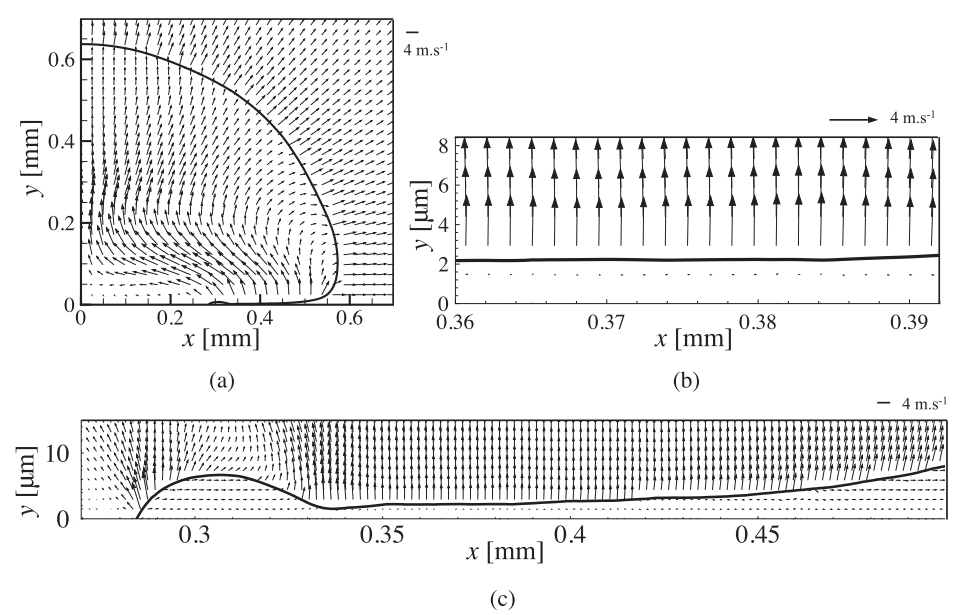
\includegraphics[width=0.7\linewidth]{img/growth/ML_urbano.PNG}
\caption{Microlayer appearing beneath the bubble in DNS conducted by and adapted from Urbano \etal \cite{urbano_direct_2018}.}
\label{fig:ML_Urbano}
\end{figure}


Parallel to the heat diffusion approach, some authors computed the bubble growth by considering a pure microlayer evaporation regime. A well-known model of this type has been derived by Cooper \& Lloyd in 1969 \cite{cooper_lloyd_1969} and considers the wall thermal properties so that:

\begin{align} 
R\parth{t} =& 2.5 \dfrac{\Ja}{\sqrt{\Pr_{L}}}\sqrt{\eta_{L}t}\ \text{if}\ \lambda_{w} \gg \lambda_{L} \\
%
R\parth{t} =& \dfrac{2}{\sqrt{\pi}} \sqrt{\dfrac{\lambda_{w}\rho_{w}c_{p,w}}{\lambda_{L}\rho_{L}c_{p,L}}}\ \text{if}\ \lambda_{w} \ll \lambda_{L}
\end{align}

\begin{remark*}{}
The parameter $ \sqrt{\dfrac{\lambda_{w}\rho_{w}c_{p,w}}{\lambda_{L}\rho_{L}c_{p,L}}}$ that accounts for the wall properties is the same used in the correlation of \"Unal for the maximum bubble diameter (Eq. \ref{eq:dlo_unal}).
\end{remark*}

The microlayer is also often taken into account for HFP modeling by enhancing the boiling heat flux through a computation of the microlayer volume \cite{kommajosyula, demarly}. 

\npar

However, the presence of a liquid microlayer beneath the nucleated bubble is not assured for every boiling conditions. Indeed, experimental observations recently realized by Kossolapov \cite{kossolapov_experimental_2021} showed that the microlayer only existed for pressures below 3 bars when using water as working fluid. Moreover, Direct Numerical Simulations of Urbano \etal \cite{urbano_direct_2018} where a full coupling between mass, momentum and energy balance was achieved managed to detect wether if the bubble grows in a contact-line regime or if a microlayer appears. They proposed a criterion based on the capillary and Jakob numbers determining the formation of a microlayer :

\begin{equation}
\frac{\Ja \Ca}{\parth{\theta-\theta_{0}}^{3}} > \frac{1}{A^{3}},\ \theta_{0}=5\degree,\ A=313
\end{equation}

\begin{remark*}{}
Computing the capillary number using $\dot{R}=\dfrac{K\Ja}{2}\sqrt{\dfrac{\eta_{L}}{t}}$ as the interface velocity, we use Urbano \etal criterion to compute the time $t_{max}$ after which the microlayer would cease to exist. Applying this to PWR conditions ($K=1$, $\Delta T_{w}=5K$) yields $t_{max}<10^{-11}$s for $6\degree \leq \theta \leq 90\degree$, meaning that there is no time during the bubble growth during which a microlayer could grow. This agrees with the observation that increasing pressure would lead to microlayer disappearance.
\end{remark*}

We will not further detail the study of the microlayer regime since its existence is very unlikely if not impossible in the pressurized conditions typical of a PWR.


\subsection{Bubble Growth in Subcooled Flow Boiling}


If we consider the full problem of bubble growth in subcooled flow boiling, the analytic expressions presented above may fall out of their validation range since extra physical phenomena will be at stake. This more generic type of growth lack of proper theoretical derivations due to the complexity of the considered system (turbulence, condensation, convection, etc.). That is why authors trying to represent such complex bubble growth often combine different heat transfer mechanisms such as: 

\begin{itemize}
\item Evaporation due to conduction from the superheated liquid near the bubble base ;
\item Evaporation of the liquid microlayer ;
\item Condensation on top of the bubble when it reaches subcooled liquid ;
\item Convective heat transfer due to relative velocity between the bubble and the liquid.
\end{itemize}

To our knowledge, such models always consider empirical or fitted parameters. For instance Yoo \etal \cite{yoo_development_2018} wrote for a sliding bubble:


\begin{align}
 \dtime{R} = &\underbrace{ \gamma \Pr_{L}^{-0.5}\Ja_{w} \sqrt{\dfrac{\eta_{L}}{t}} \frac{A_{ML}}{A_{b}} }_{\text{Microlayer}} + \underbrace{\parth{1-f} \frac{b}{\sqrt{\pi}} \Ja_{w} \sqrt{\dfrac{\eta_{L}}{t}}}_{\text{Superheated liquid}} - \underbrace{\frac{f\Delta T_{L}C}{1-\rho_{V}/\rho_{L}}R}_{\text{Subcooled convection}}
\label{eq:growth_yoo}
\end{align}
where $\gamma = \sqrt{\dfrac{\lambda_{w}\rho_{w}c_{p,w}}{\lambda_{L}\rho_{L}c_{p,L}}}$, $\dfrac{A_{ML}}{A_{b}}=1.22 \gamma^{-0.79}\exp{-0.204\Ja_{w}}$, $f=0.5$, $b=0.24$ and $C=0.1$.

\npar
Their model was validated against low pressure sliding of boiling bubbles for different fluids (Water \cite{maity_effect_2000}, FC87 \cite{thorncroft_experimental_1998}, R113 \cite{yoo_exp_2016}). They account for wall properties through the parameter $\gamma$ in the microlayer term while assuming that 50\% of the bubble faces subcooled liquid ($f=0.5$) and condenses following the formulation of Levenspiel \cite{levenspiel_collapse_1959}.


\npar

Zhou \etal \cite{zhou_experimental_2020} also proposed a similar modeling of the bubble growth, validated on their own measurements for boiling water at low pressure:


\begin{align}
\nonumber \dtime{R} = &\underbrace{ \frac{1}{C} \Pr_{L}^{-0.5}\Ja_{w} \sqrt{\dfrac{\eta_{L}}{t}} }_{\text{Microlayer}} + \underbrace{\sqrt{\dfrac{3}{\pi}}\Ja_{T} \sqrt{\dfrac{\eta_{L}}{t}}\min{\dfrac{y_{sat}}{2R},\ 1}}_{\text{Superheated liquid}}\\ 
%
& - \underbrace{\frac{\eta_{L}}{2R}\Ja_{L}\parth{2+0.6\Re_{b}^{0.5}\Pr_{L}^{0.3}}\max{\frac{H-y_{sat}}{2R},\ 0}}_{\text{Subcooled convection}}
\end{align}
where $C=1.45$, $\Ja_{T}$ is the Jakob number taken at $\min{\overline{T}-T_{sat},\ 0}$, $\overline{T}$ the average liquid temperature around the bubble, $H=R\parth{1+\cos{\theta}}$.

\npar

While they consider a constant coefficient for the microlayer evaporation, they propose a finer modeling of the condensation term by evaluating the height $y_{sat}$ at which $T_{L}=T_{sat}$ using the turbulent wall law of Kader \cite{kader_wall_law_1969}. The condensation is modeled by the Ranz \& Marshall correlation \cite{ranz_marshall} that accounts for the relative velocity through the bubble Reynolds number.


\begin{remark*}{}
As mentioned before, those model rely on numerous empirical parameters due to the variety of considered phenomena. In particular, microlayer evaporation is systematically considered which could be questioned regarding the observations made in Subsection \ref{subsec:microlayer}.
\end{remark*}

\npar

Contrary to those models, Mazzocco \etal \cite{mazzocco_reassessed_2018} propose to keep the radius as $K\Ja_{w}\sqrt{\eta_{L}t}$ and to include subcooling and microlayer influence in the value of $K$:

\begin{equation}
K = \frac{1.243}{\sqrt{\Pr_{L}}} + 1.945*\chi,\ \chi = 1-B\frac{\Delta T_{L}}{\Delta T_{w}}
\label{eq:Kgrowth_mazzocco}
\end{equation}
with $A=0.05$ and $B=1.55$ based on data-fitting.

\begin{remark*}{}
This approach in interesting because it keeps the simple growth law in $t^{1/2}$ but the definition of $\chi$ is hardly general since it can lead to $K\leq 0$ for high values of $\dfrac{\Delta T_{L}}{\Delta T_{w}}$ which would be unphysical.
\end{remark*}


\subsection{Analytic Approach of Bubble Growth in a Linear Thermal Boundary Layer}

In this Subsection, we propose an analytic derivation of bubble growth for a truncated sphere laying on a wall in a boundary layer with a linear temperature profile. The considered geometrical and thermal definitions are depicted on Figure \ref{fig:anal_growth}.


\begin{figure}[h!]
\centering
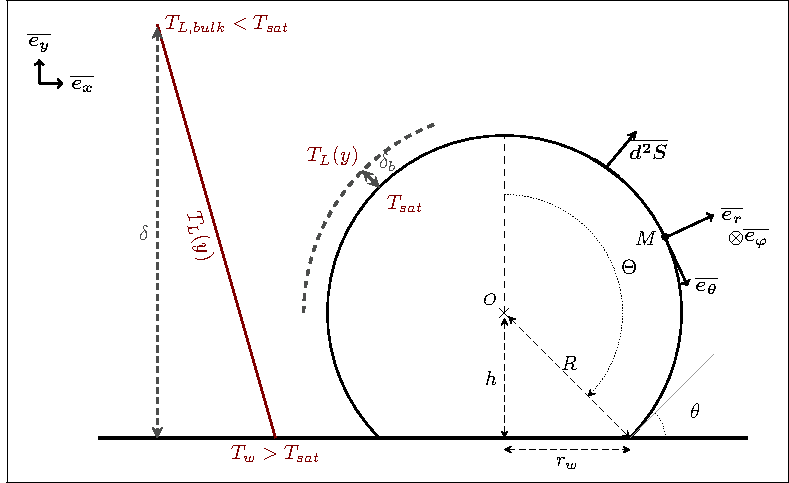
\includegraphics[width=0.7\linewidth]{img/growth/growth_analytical.pdf}
\caption{Studied geometry}
\label{fig:anal_growth}
\end{figure}

We consider an established single-phase thermal boundary layer of thickness $\delta$. When the bubble start to grow, an other boundary layer will of thickness $\delta_{b}$ grow between the liquid-vapor interface and the surrounding liquid which temperature depends on the wall distance $y$.


\npar


The liquid temperature is is assumed to follow a linear profile:

\begin{align}
T_{L}\parth{y}=T_{w}+\frac{T_{L,bulk}-T_{w}}{\delta} y
\end{align}


Assuming that the vapor stays at a temperature close to $T_{sat}$, the radial component of the temperature gradient at the bubble's interface can be expressed as:

\begin{align}
\grad{T} \cdot \vect{e_{r}} = \dpartial{T}{r}\parth{R, \vartheta, \varphi} \approx\frac{T_{L}(y)-T_{sat}}{\delta_{b}}
\end{align}

\npar



Applying Fourier's law to the liquid close to the bubble to estimate the heat flux density vector $\vect{j_{Q}}=-\lambda_{L} \grad{T}$. Between $t$ and $t+dt$ the heat exchanged through $d^{2}S$ is:

\begin{align}
d^{2}Q_{b} \approx -\frac{\lambda_{L}}{\delta_{b}}\crocht{ \Delta T_{w}R^{2}\sin{\vartheta}-\frac{\Delta T_{w}+\Delta T_{L}}{\delta}R^{3}\crocht{ \cos{\vartheta}-\cos{\varTheta} } \sin{\theta} } \mathrm{d}\vartheta \mathrm{d}\varphi
\end{align}

\npar
Then assuming that $\delta_{b}$ is constant between $t$ and $t+dt$, the total heat flux can be expressed by integrating over the bubble's surface:

\begin{align}
Q_{b}=\frac{2\pi \lambda_{L} R^{2}}{\delta_{b}} \parth{1+\cos{\theta} } \crocht{\Delta T_{w} - \frac{R}{2\delta}\parth{ \Delta T_{w} + \Delta T_{L} }  \parth{1 + \cos {\theta}} }
\end{align}

Writing the mass balance by considering that the heat flux contributes solely to phase change:

\begin{align}
\dtime{V_{b}}=\frac{Q_{b}}{\rho_{V}h_{LV}}
\end{align}

\begin{equation}
V_{b} = \frac{4}{3}\pi R^{3} f_{V},\ f_{V} = \frac{1}{4}\parth{2-\cos{\theta}}\parth{1+\cos{\theta}}^{2}
\end{equation}

Writing this in terms of bubble radius:

\begin{align}
\dtime{R} = \frac{\Ja_{w} \eta_{L}}{2 \delta_{b} f_{V} } \parth{1+\cos{\theta}} \crocht{1 - \frac{R}{2\delta}\parth{ 1 + \frac{\Ja_{L}}{\Ja_{w}} } \parth{ 1 + \cos{\theta} } }
\end{align}

Which reduces to the following differential equation:

\begin{equation}
\dtime{R} + aR = b
\label{eq:diff_eq_growth}
\end{equation}

\begin{equation}
a = \frac{\Ja_{w}\eta_{L}}{4 \delta_{b} \delta f_{V} } \parth{1 + \frac{\Ja_{L}}{\Ja_{w}} } \parth{1 + \cos{\theta} }^{2} \ \text{and} \  b = \frac{\Ja_{w}\eta_{L}}{2 \delta_{b} f_{V} }\parth{1 + \cos{\theta} }
\end{equation}


\npar

Solutions of this differential equation depend on the hypothesis over $\delta$ and $\delta_{b}$. If we assume that the bubble grows in a fully established liquid flow then $\delta$ can be considered as constant.

When the bubble will start to nucleate, the liquid-vapor interface will delimit a frontier through which a transient heat transfer between the vapor at constant temperature $T_{sat}$ and liquid at $T_{L}\parth{y}$ will occur. To estimate the associated local boudary layer thickness $\delta_{b}$, we can rely on the solution of semi-infinite transient conduction as treated in Del Valle \& Kenning \cite{delvalle_quenching} or Mikic \& Rohsenow \cite{mikic_1970}:

\begin{equation}
\delta_{b} = \sqrt{\eta_{L}t}
\label{eq:TBL_expgrowth}
\end{equation}

\npar

The differential equation Eq. \ref{eq:diff_eq_growth} becomes:

\begin{align}
\dtime{R}+a\parth{t}R=b\parth{t}
\end{align}

\begin{align}
a(t)=&\frac{\Ja_{w}\sqrt{\eta_{L}}}{4\delta f_{V}\sqrt{t}}\parth{1+\frac{\Ja_{L}}{\Ja_{w}}}\parth{1+\cos{\theta}}^{2}=K_{a}t^{-1/2} \\
b(t)=&\frac{\Ja_{w}\sqrt{\eta_{L}}}{2f_{V} \sqrt{t}}\parth{1+\cos{\theta}}=K_ {b}t^{-1/2}
\label{eq:coeff_expgrowth}
\end{align}

\npar

With the initial condition $R\parth{t=0}=0$, the solution to this differential equation is: 

\begin{align}
R\parth{t}=&R_{\infty}\parth{1-e^{-2K_{a}\sqrt{t}}}
\label{eq:exp_growth} \\
R_{\infty}=&\frac{K_{b}}{K_{a}} = \frac{2\ \delta}{\parth{1+\dfrac{\Ja_{L}}{\Ja_{w}} } \parth{1+\cos{\theta} } }
\label{eq:eq_radius_expgrowth}
\end{align}

\npar

This type of bubble growth presents interesting properties. First, it degenerates to the uniformly superheated liquid solution when $t \to 0$:

\begin{equation}
R\parth{t} \underset{t \to 0}{\thicksim} \frac{1+\cos{\theta}}{f_{V}}\Ja_{w} \sqrt{\eta_{L}t}
\end{equation}
with a purely geometrical growth constant depending on the contact angle, equal to $2$ for the spherical case.

\npar
Moreover, this growth law accounts for the liquid subcooling and thus presents an equilibrium radius $R_{\infty}$ when $t\to \infty$, corresponding to the bubble size at which the vaporization from the superheated liquid is exactly compensated by the condensation at the bubble top.

\npar
To the best of our knowledge, this simple bubble growth law has never been proposed in the literature. However, this equation has some limitations :

\begin{itemize}
\item It requires the knowledge of the liquid thermal boundary layer thickness $\delta$ which estimation can be tricky ;

\item This law can't be applied if $T_{L,bulk}>T_{sat}$.
\end{itemize} 


\begin{remark*}{}
It is worthy to note that this solution is derived solely using the energy balance at the liquid-vapor interface. No momentum balance was used when solving this physical problem, which can be considered as a limit of the approach.
\end{remark*}


\subsection{Comparison with DNS Results}

To assess the validity of Eq. \ref{eq:exp_growth}, we will compare the radius time profile with DNS results by Urbano \etal \cite{urbano_2019} who simulated the same physical situation as depicted in Figure \ref{fig:anal_growth} for pool boiling. They also solved the heat conduction in the wall and studied the the growth dynamics depending on the values of $\Delta T_{L}$ and $\Delta T_{w}$ as well as the equilibrium diameter reached by the bubble.

\npar

In their analysis, Urbano \etal derived the same equilibrium radius as in Eq. \ref{eq:eq_radius_expgrowth} by equating the condensation and vaporization heat fluxes. By comparing with the equilibrium radius reached in their simulations, they found that a corrective factor $C=1.15829$ was needed to correct Eq. \ref{eq:eq_radius_expgrowth}. This difference could be explained by the heat conduction in the wall that is not accounted for in the theoretical approach.

\npar

DNS results obtained for three couples of subcooling $\Delta T_{L}$ and superheat $\Delta T_{w}$ are used for comparison. Results are displayed on Figure \ref{fig:growth_comp_urbano} with and withouth the corrective factor on $R_{\infty}$ suggested by Urbano \etal

\begin{figure}[h!]
\subfloat[Results using $R_{\infty}$]{
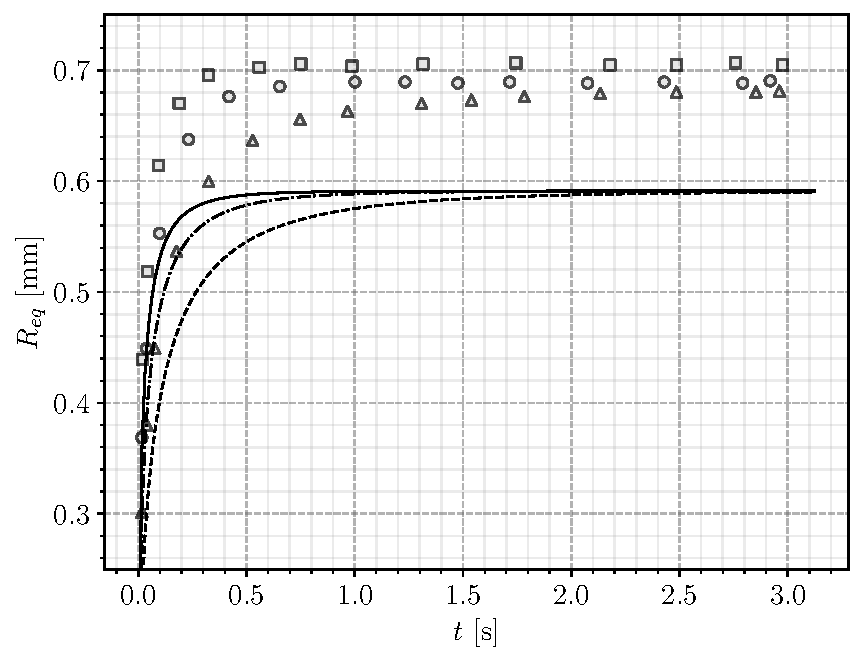
\includegraphics[width=0.5\linewidth]{img/growth/comp_urbano_nocorr.pdf}
}
\subfloat[Results using $C\times R_{\infty}$, $C=1.158$]{
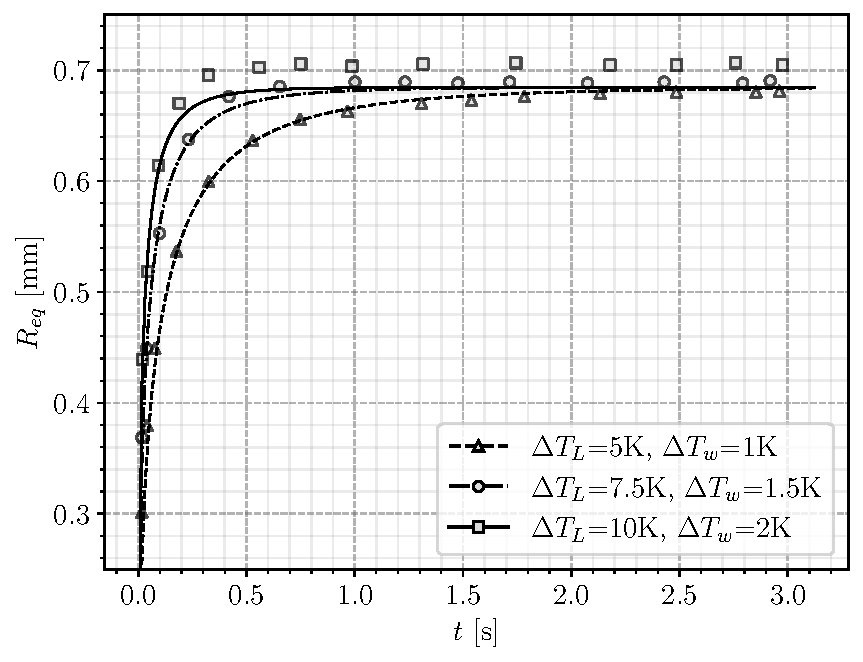
\includegraphics[width=0.5\linewidth]{img/growth/comp_urbano_corr.pdf}
}
\caption{Comparison with DNS results of Urbano \etal \cite{urbano_2019} ($\delta=3$mm and $\theta=50\degree$).\\ Lines : Model predictions - Markers : DNS }
\label{fig:growth_comp_urbano}
\end{figure}

The analytical formulation of the bubble growth matches very well with the DNS results when the equilibrium radius is corrected. The different growth regime induced by the pairs $\parth{\Delta T_{L},\ \Delta T_{w}}$ are correctly captured by the model. DNS results present different equilibrium radius values when the subcooling and superheat changes, which can not be accounted for by the model.

\npar

\begin{remark*}{}
Those results are encouraging and validate the modeling of $\delta_{b}$ with the semi-infinite conduction model (Eq. \ref{eq:TBL_expgrowth}).
\end{remark*}



\subsection{Comparison with Experimental Measurements}

\subsubsection{Low Pressure Measurements}
To further evaluate the proposed model, we compare the result with experimental measurements of bubble radius in vertical boiling of water at atmospheric pressure by Maity \cite{maity_effect_2000}. The choice of $\delta$ is adapted to each case and $\theta=45\degree$ is the average measured contact angle in the experiments.

In addition, we also plot the predictions by the heat diffusion solution $R=K\Ja_{w}\sqrt{\eta_{L}t}$ with $K=\dfrac{2b}{\sqrt{\pi}}$ and $1 \leq b \leq \sqrt{\pi}$. A solution with an optimized value of $K$ is also represented. The models of Mazzocco and Yoo \etal are also compared. 

The results are presented on Figure \ref{fig:growth_comp_maity}.

\begin{figure}[h!]
\subfloat[$G_{L}=0~ \debm$, $\Delta T_{w}=5.9K$, $\Delta T_{L}=0.7K$]{
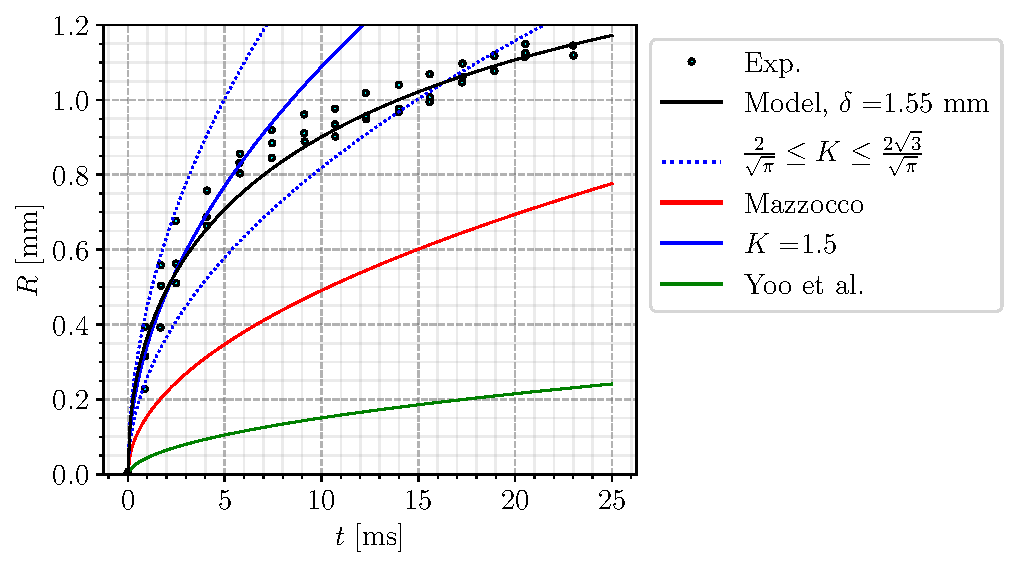
\includegraphics[width=0.5\linewidth]{img/growth/maity_V0.pdf}
}
\subfloat[$G_{L}=73.8~ \debm$, $\Delta T_{w}=5.0K$, $\Delta T_{L}=0.6K$]{
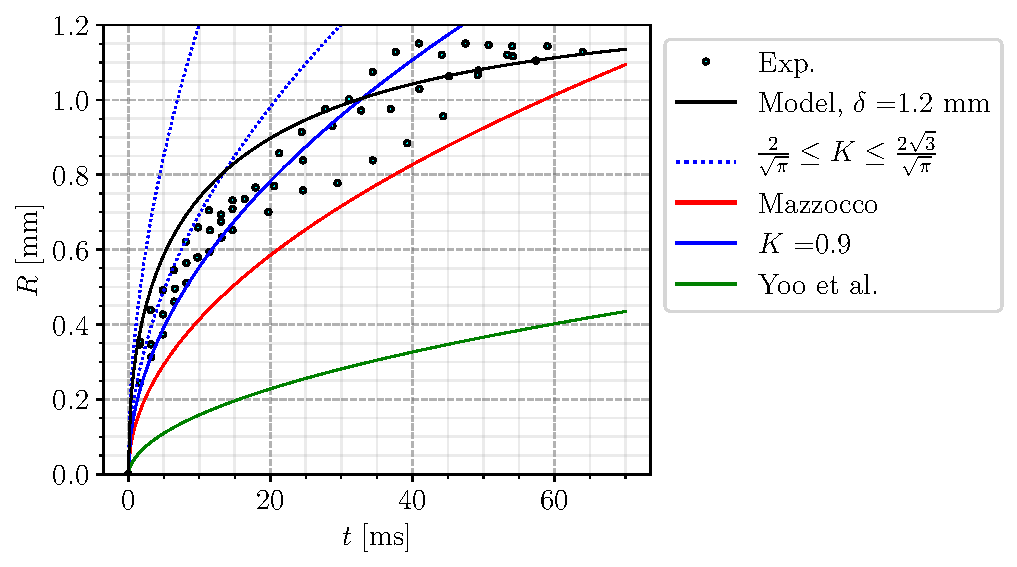
\includegraphics[width=0.5\linewidth]{img/growth/maity_V0p077.pdf}
}
\\
\subfloat[$G_{L}=143.8~ \debm$, $\Delta T_{w}=5.9K$, $\Delta T_{L}=0.3K$]{
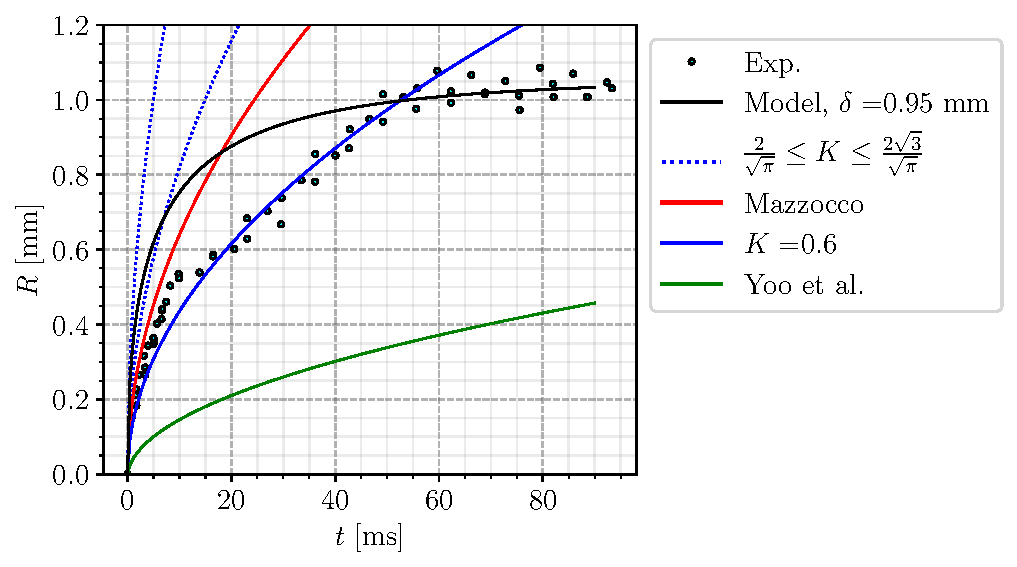
\includegraphics[width=0.5\linewidth]{img/growth/maity_V0p15.pdf}
}
\subfloat[$G_{L}=239.6~ \debm$, $\Delta T_{w}=5.9K$, $\Delta T_{L}=0.3K$]{
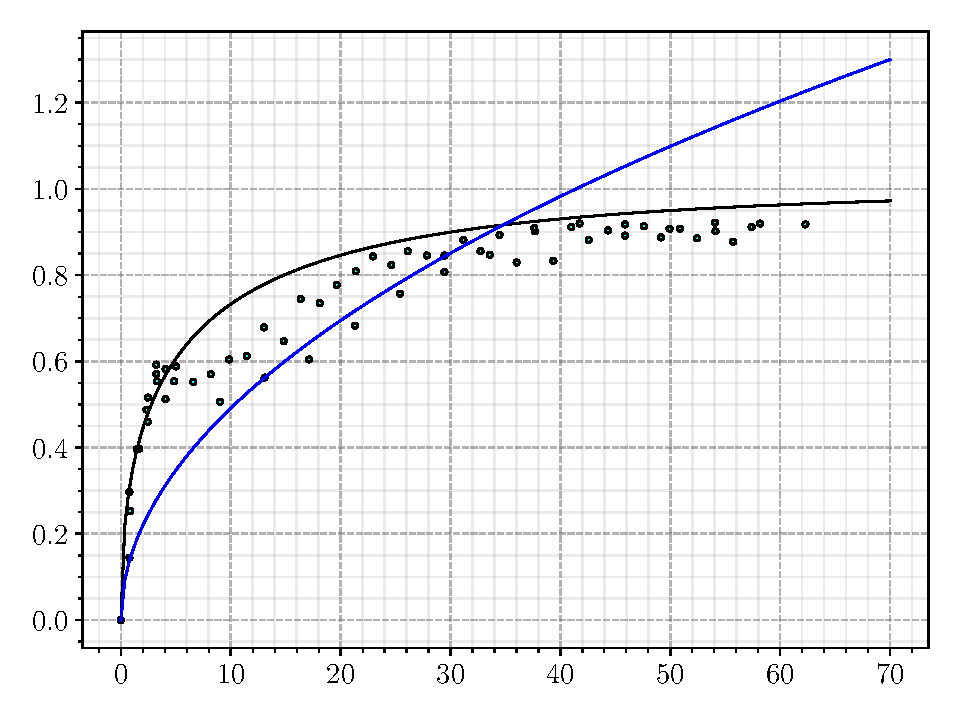
\includegraphics[width=0.5\linewidth]{img/growth/maity_V0p25.pdf}
}
\caption{Comparison with experimental measurements of Maity  \cite{maity_effect_2000}.}
\label{fig:growth_comp_maity}
\end{figure}


The new formulation globally reproduces the experimental results better than the other models. In particular, the progressively damped growth rate when the bubble start to face colder liquid seems to correctly captures the nonlinear experimental growth. Values of $\delta$ needed to produce those results were between $0.85$ mm and $1.55$mm, which reasonably agrees with measurements of Maity in his experiment for horizontal flow giving $\delta$ roughly between $1$ mm and $1.5$ mm.

\begin{remark*}{}
We can note that the optimal value of $\delta$ decreases as liquid mass flux increases, which is physically coherent as the thermal boundary layer will diminish in size with the Reynolds number.
\end{remark*}

\npar

On the other hand, the fitted value of $K$ is often smaller than the lower bound $\dfrac{2}{\sqrt{\pi}}$ suggested by Zuber \cite{zuber_dynamics_1961}. This is a consequence of the subcooled flow which deviates from the uniformly superheated liquid from which those values were derived. This fitted profile manages to capture some stages of bubble growth but can not predict the asymptotic behavior where bubble reaches a quasi-constant radius.

We see that the growth constant computed by Mazzocco \etal (Eq. \ref{eq:Kgrowth_mazzocco}) produce slightly better results compared to the analytic values of $K$ but can lead to underestimations as for the pool boiling case.

\npar

Finally, we see that the model of Yoo \etal underestimates the bubble radius. We suspect this could come from the assumption considering that half of the bubble faces subcooled liquid ($f=0.5$, Eq. \ref{eq:growth_yoo}), which is hardly reasonable especially at early growth stages.



\subsubsection{High Pressure Measurements}

The model is now compared to higher pressure measurement (20 bar and 40 bar) for water boiling by Kossolapov \cite{kossolapov_experimental_2021}. All the experiments are conducted with $10$K of subcooling, and we take a contact angle of $\theta=80\degree$ (typical for water and ITO). The range of the measured diameters over time are represented since Kossolapov observed the growth of thousands of bubbles over the heater surface. Results are presented on Figure \ref{fig:comp_growth_koss}. We could not compare the model of Mazzocco because the formulation of Eq. $\ref{eq:Kgrowth_mazzocco}$ yielded negative growth constant.



\begin{figure}[h!]
\begin{center}
\subfloat[$P=20$ bar, $G_{L}=500\ \debm$,\\ $\phi_{w} = 0.178$~MW/m\up{2}, $\Delta T_{w}=12.6$K]{
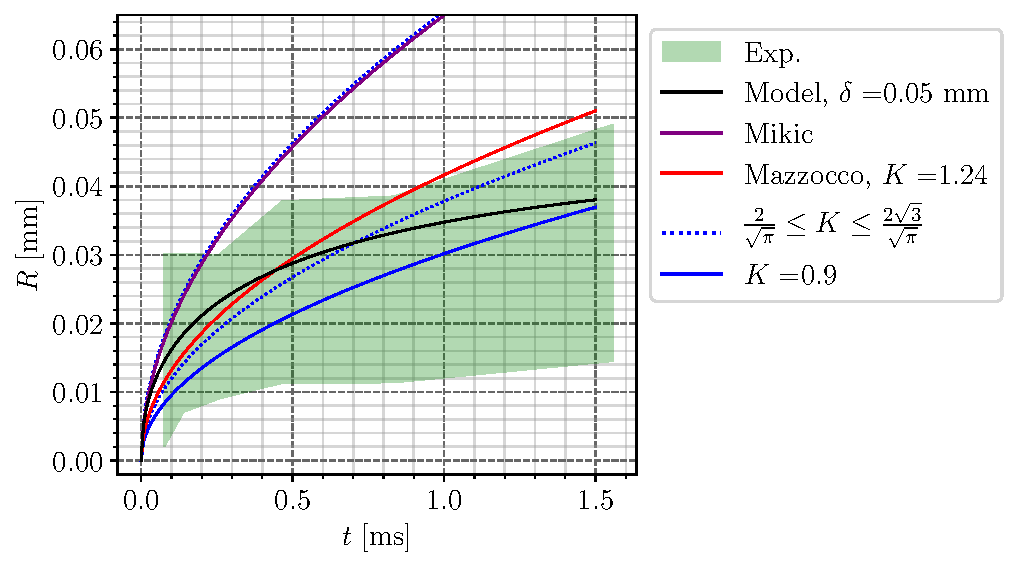
\includegraphics[width=0.5\linewidth]{img/growth/Koss_P20_G500.pdf}
} 
\subfloat[$P=40$ bar, $G_{L}=500\ \debm$,\\ $\phi_{w} = 0.291$~MW/m\up{2}, $\Delta T_{w}=10.1$K]{
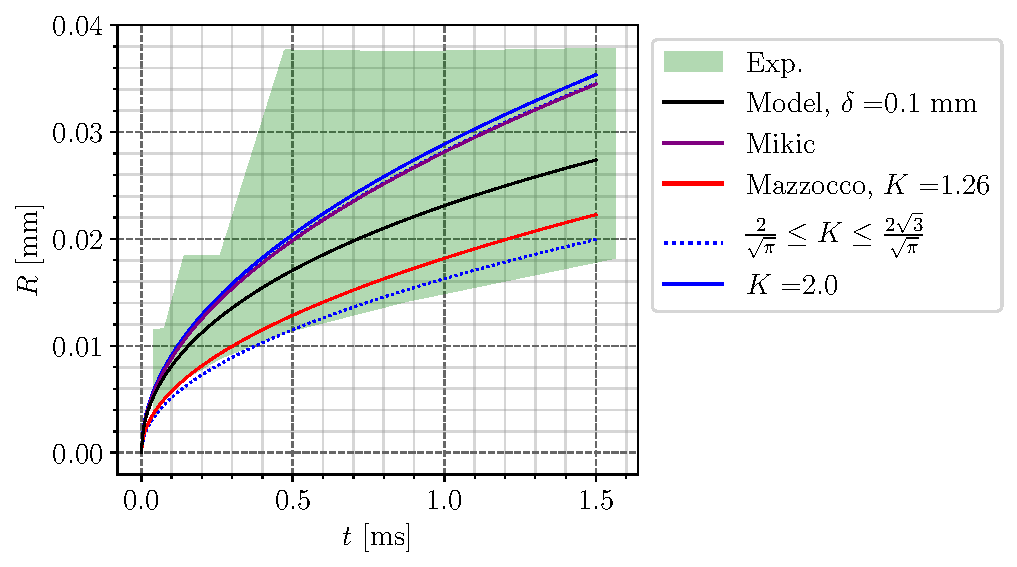
\includegraphics[width=0.5\linewidth]{img/growth/Koss_P40_G500.pdf}
}
\\
\subfloat[$P=20$ bar, $G_{L}=994\ \debm$,\\ $\phi_{w} = 0.495$~MW/m\up{2}, $\Delta T_{w}=16.1$K]{
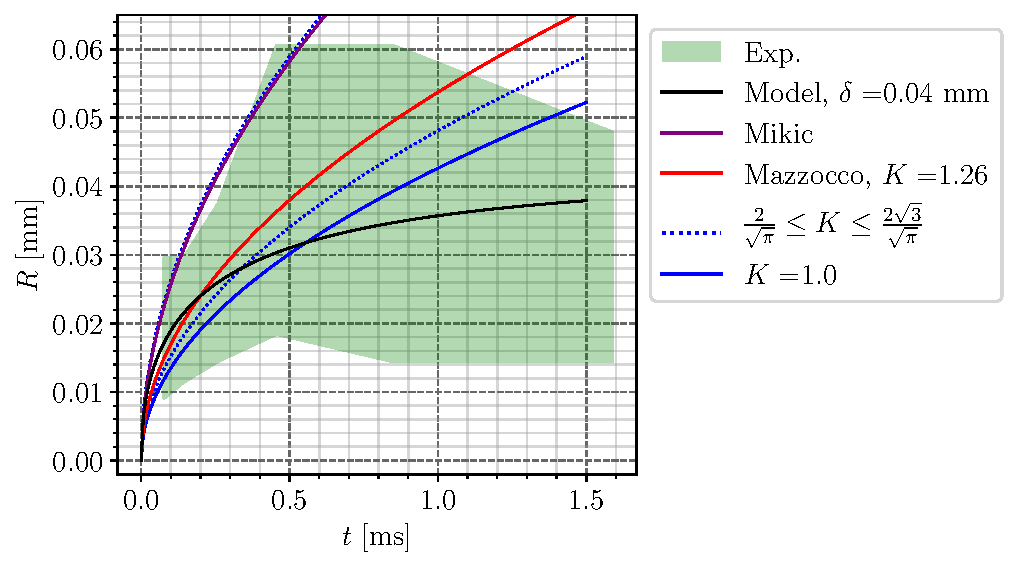
\includegraphics[width=0.5\linewidth]{img/growth/Koss_P20_G1000.pdf}
} 
\subfloat[$P=40$ bar, $G_{L}=994\ \debm$,\\ $\phi_{w} = 0.361$~MW/m\up{2}, $\Delta T_{w}=10.8$K]{
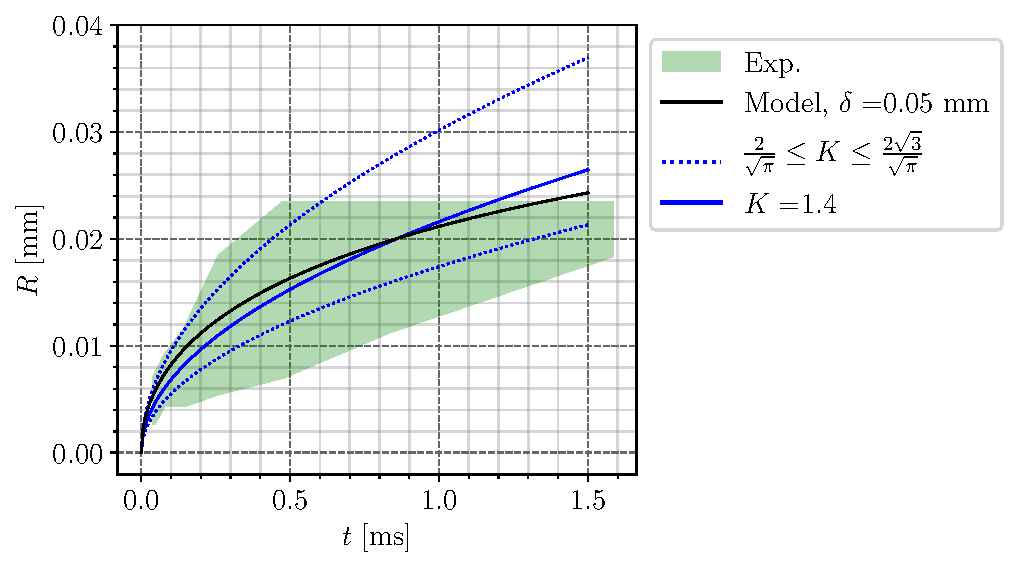
\includegraphics[width=0.5\linewidth]{img/growth/Koss_P40_G1000.pdf}
}
\\
\subfloat[$P=20$ bar, $G_{L}=1504\ \debm$,\\ $\phi_{w} = 0.487$~MW/m\up{2}, $\Delta T_{w}=16.2$K]{
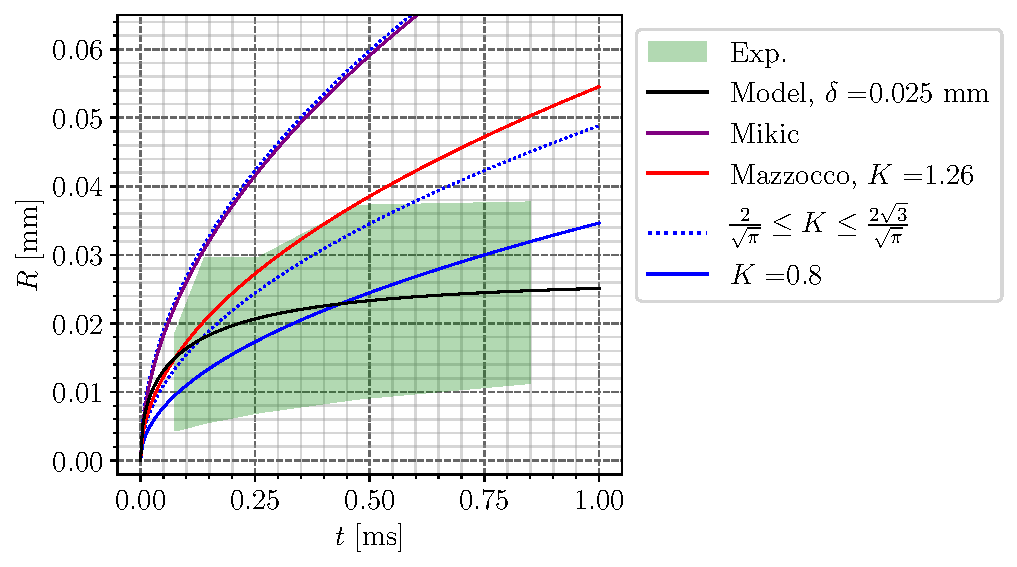
\includegraphics[width=0.5\linewidth]{img/growth/Koss_P20_G1500.pdf}
} 
\subfloat[$P=40$ bar, $G=1504\ \debm$,\\ $\phi_{w} = 0.613$~MW/m\up{2}, $\Delta T_{w}=12.2$K]{
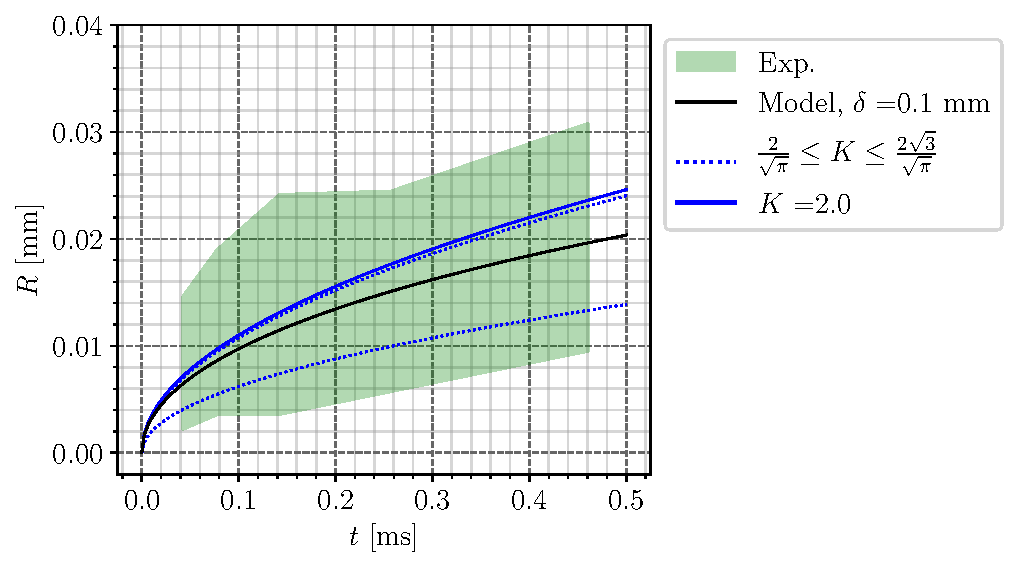
\includegraphics[width=0.5\linewidth]{img/growth/Koss_P40_G1500.pdf}
}


	\caption{Comparison with experimental measurements of Kossolapov \cite{kossolapov_experimental_2021}. $\Delta T_{w}$ values are recalculated from analytical growth profiles fitted by the author.}
	\label{fig:comp_growth_koss}
\end{center}
\end{figure}


The values of $\delta$ needed to match the experimental measurements using Eq. \ref{eq:exp_growth} are much smaller than the low pressure case, with $\delta \leq 0.1$ mm. The higher mass fluxes in Kossolapov measurements could explain lower values of $\delta$, nevertheless they do not follow a particular trend with $G_{L}$.

\npar

Contrary to low pressure measurements, the Plesset \& Zwick solution with $\dfrac{2}{\sqrt{\pi}} \leq K \leq \dfrac{2\sqrt{3}}{\sqrt{\pi}}$ provides an acceptable estimation of the bubble radius. This is probably due to the smaller bubble size in pressurized boiling (roughly 10 times smaller compared to atmospheric pressure).

\begin{remark*}{}
The non-dimensional distances associated to the bubble radius $R^{+}=\dfrac{R u_{\tau}}{\nu_{L}}$ rise up to 40 for Maity cases and 20 for Kossolapov cases while having way larger liquid mass fluxes. This supports the fact that bubbles are higher pressure are less likely to be impacted by subcooled liquid, spending most of their lifetime between the viscous and buffer layer.
\end{remark*}


\subsection{Conclusions on Bubble Growth Modeling}

\begin{itemize}

\item Recent experimental and numerical research have shown that the presence of a liquid microlayer contributing to the bubble growth strongly depends on the boiling conditions. In particular, disappearance of this microlayer ate pressures higher than $3$ bar have been observed by Kossolapov \cite{kossolapov_experimental_2021}. This microlayer should thus not be systematically taken into account.

\item A new formulation derived from the heat diffusion in a linear temperature profile has been proposed (Eq. \ref{eq:exp_growth}). Provided a correct value of the thermal boundary thickness $\delta$, validation both on DNS and low pressure measurements shows that the model better captures the growth regime of bubbles in subcooled boiling compared to traditional models. However, this improvement appears limited at higher pressure when bubbles are smaller, where the Plesset \& Zwick treatment also proposes an acceptable estimation of the bubble growth.

\item Mechanistic models that includes several heat transfer mechanisms require a certain number of empirical closures that limits the model generality, making them unsuitable for application to any boiling conditions.

\item Whatever the conditions, a proper choice of the growth constant $K$ in the $R=K\Ja_{w} \sqrt{\eta_{L}t}$ solution for a uniform liquid superheat can yield reasonable results. Moreover, it presents interesting mathematical properties such as the time independence of the products $R \dot{R}$ and $R^{3}\ddot{R}$ that appear in the bubble force balance (Eq. \ref{eq:bdf_y}).

\end{itemize}

All things considered, it seems that the proposed new growth law of Eq. \ref{eq:exp_growth} can be of greater interest for low pressure boiling where larger bubbles are more impacted by the bulk flow. Although it provides finer physical representation of bubble radius evolution, its application is limited by the estimation of $\delta$ to which the model is strongly sensitive. \textbf{On the other hand, less precise yet acceptable predictions of bubble growth are achieved using the $t^{1/2}$ law with a growth constant $K$ close to unity.}




\section{Departure by Sliding}\label{sec:departure}

The question of departure by sliding being central for bubble dynamics in vertical flow boiling, we will tackle the problem by starting with a non-dimensional analysis before moving to predictions of experimental measurements of departure diameters.

\subsection{Non-Dimensional Analysis}\label{subsec:adim_dep}

To study the departure by sliding, we rely on force balance parallel to the wall (Eq. \ref{eq:bdf_x}). Before departure, the bubble grows on its nucleation site while staying immobile, thus with a sliding velocity $U_{b} = \dfrac{ \partial U_{b}}{\partial t} =0$. The force balance parallel to the wall becomes:

\begin{align}
- \pi R\sigma f_{C,x} + \frac{4}{3}\pi R^{3}\parth{\rho_{L}-\rho_{V}}g &+ \frac{1}{2}C_{D}\rho_{L}\pi R^{2} U_{L}^{2} + \frac{4}{3}\pi R^{3}\rho_{L}~3C_{AM,x}\frac{\dot{R}}{R}U_{L} = 0
\label{eq:bdf_x_dep}
\end{align}


We can note that in this equation, departure by sliding is promoted by the buoyancy, the drag and the added mass forces. Only the capillary force keeps the bubble attached to its nucleation site, which will be discussed later.
As discussed in the previous section, the bubble growth is modeled as:

\begin{equation}
R\parth{t} = K\Ja_{w} \sqrt{\eta_{L}t}
\end{equation}
with $K$ as an adjustable constant.

\npar
Re-writing Eq.~\ref{eq:bdf_x_dep} in non-dimensional form by dividing the LHS by the added mass force yields:

\begin{equation}
-\frac{1}{2}\frac{f_{C,x}}{K^{2}C_{AM,x}}\frac{1}{\Ca}\frac{\Pr_{L}}{\Ja_{w}^{2}} +  \frac{1}{3}\frac{1}{K^{2}C_{AM,x}}\frac{\Re_{b}}{\Fr}\frac{\Pr_{L}}{\Ja_{w}^{2}} + \frac{1}{8}\frac{C_{D}}{K^{2}C_{AM,x}}\Re_{b}\frac{\Pr_{L}}{\Ja_{w}^{2}} +1 =0
\label{eq:adim_dep}
\end{equation}
where we have the following non-dimensional numbers:
\begin{align}
\nonumber \Re_{b} =& \frac{2RU_{L}}{\nu_{L}}\ ;\ \Fr=\frac{\rho_{L}U_{L}^{2}}{\parth{\rho_{L}-\rho_{V}}g R}\ ;\ \We=\frac{\rho_{L}U_{L}^{2}R}{\sigma}\ ; \ \Eo=\frac{\parth{\rho_{L}-\rho_{V}}g R^{2}}{\sigma}\ ;\\
%
\nonumber \Ja_{w}=&\frac{\parth{T_{w}-T_{sat}}\rho_{L} c_{P,L}}{\rho_{V} h_{LV}}\ ;\ \Pr_{L}=\frac{\nu_{L}}{\eta_{L}}\ ;\ \frac{\dot{R}}{U_{L}}=\frac{K^{2}\Ja_{w}^{2}}{\Pr_{L} \Re_{b}}\ ;\ \Ca=\frac{\mu_{L}U_{L}}{\sigma}
\end{align}
%=\Re_{b}^{2}\frac{\rho_{L}\nu_{L}^{2} }{g\parth{\rho_{L}-\rho_{V}}4R^{3}} 


Eq.~\ref{eq:adim_dep} exhibits terms that can be used to compare the magnitude of each detaching forces and obtain the following conditions:

\begin{align}
&\text{Added mass  force greater than drag if:}\ \ \frac{\Ja_{w}^{2}}{\Pr_{L}}>\frac{1}{8}\frac{C_{D}}{C_{AM,x}}\frac{1}{K^{2}}\Re_{b} \label{eq:AMvsD}\\
&\text{Added mass greater than buoyancy if:}\ \  \frac{\Ja_{w}^{2}}{\Pr_{L}}>\frac{1}{3}\frac{1}{C_{AM,x}K^{2}}\frac{\Re_{b}}{\Fr} \label{eq:AMvsB}\\
&\text{Drag greater than buoyancy if:}\ \  \Re_{b}>\frac{16}{3}\frac{1}{C_{D}}\frac{\Eo}{\Ca}=\Re_{c} \label{eq:DvsB}
\end{align}

Those three conditions can be seen as boundaries in a $\parth{\Ja_{w}^{2}/\Pr\ ;\ \Re_{b}}$ plane. With a given fluid and bubble diameter $D=2R$, we can represent the different regimes of force dominance by plotting those three boundaries simultaneously on a regime map. An example of such a map is presented on Figure \ref{fig:ND_map1}.

\begin{figure}[h!]
\centering
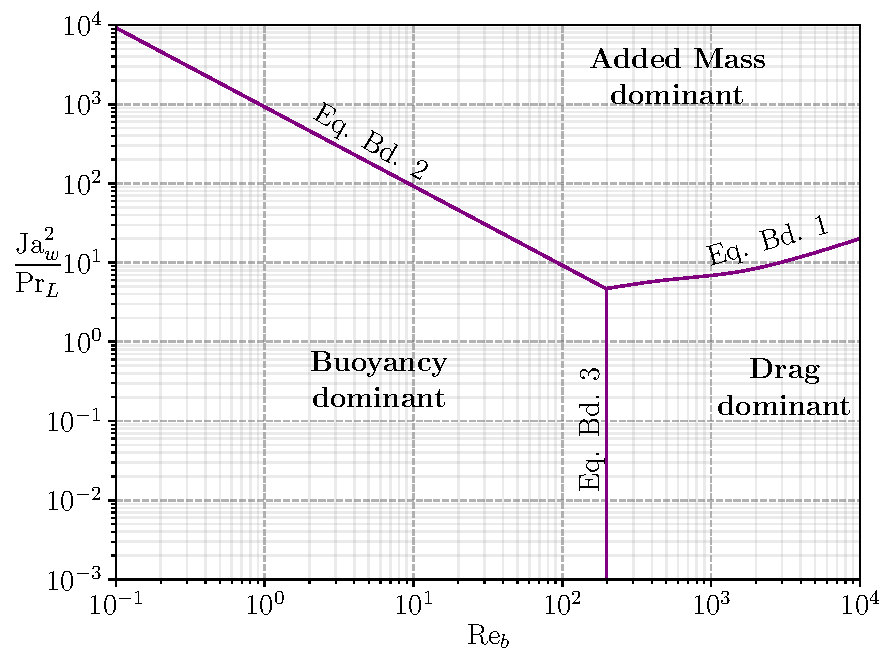
\includegraphics[width=0.6\linewidth]{img/bub_dyn/dep_maps/ND_map1.pdf}
\caption{Regime map regarding departure by sliding. Boundaries plotted for water at 1 bar and $D_{d}=0.5$mm. ($K=2$)}
\label{fig:ND_map1}
\end{figure}


This allows to visualize the operating conditions under which each of the detaching forces will be dominant. Logically, buoyancy dominates for low $\Re_{b}$ regimes contrary to drag. Added mass dominates when values of $\Ja_{w}^{2}/\Pr_{L}$ are high \ie when bubble grows rapidly.
 


\subsubsection{Influence of Pressure}

On Figure \ref{fig:press_map}, we draw the regime map for 3 different pressures and associated orders of magnitude of bubble departure diameter \cite{kocamustafaogullari_pressure_1983}.


\begin{figure}[h!]
\centering
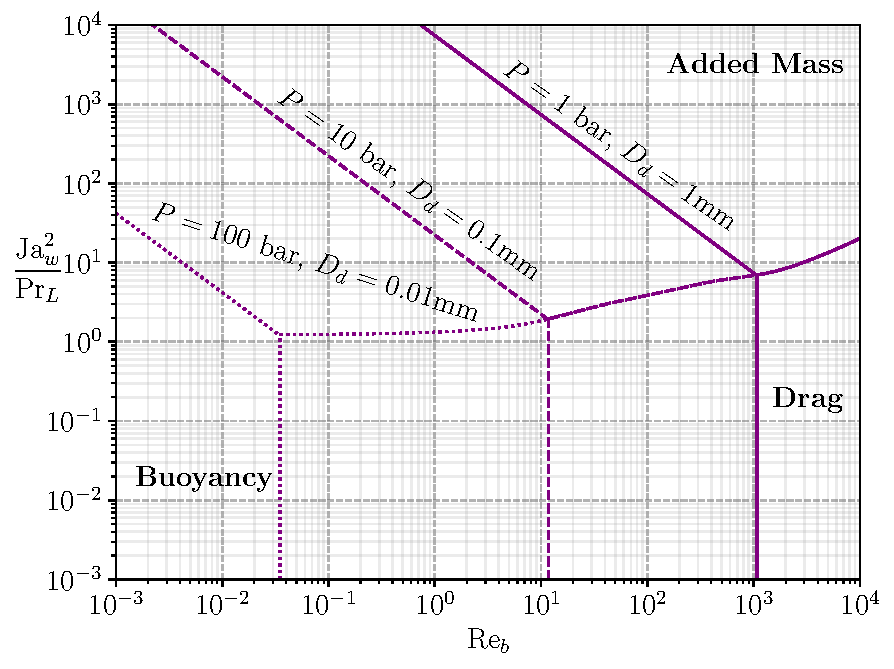
\includegraphics[width=0.6\linewidth]{img/bub_dyn/dep_maps/press_map.pdf}
\caption{Regime map plotted for water at different pressures and bubble departure diameters. ($K=2$)}
\label{fig:press_map}
\end{figure}


The impact of pressure is mostly seen through the decrease of bubble departure diameter. As pressure increases, buoyancy force decreases while drag and added mass forces display much larger dominance zones. The competition between those two terms mainly relies on the competition between liquid flow velocity and wall superheat or heat flux.

 
\subsubsection{Comparison between Fluids}

 
On Figure \ref{fig:R12_PWR_map}, we compare the dominance zones for R12 at 26 bar and water at 155 bar. Moderately pressurized R12 (10 to 30 bar) has often been used as a simulating fluid to mimic water in PWR since it has the same density ratio and Weber number for instance (see Section \ref{sec:debora} related to the DEBORA experiments).

\begin{figure}[h!]
\centering
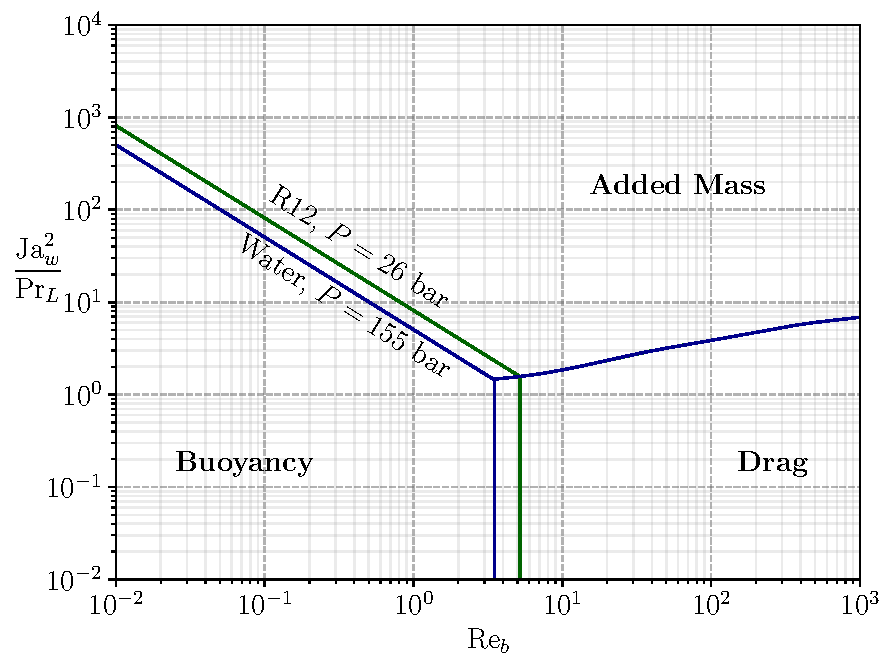
\includegraphics[width=0.6\linewidth]{img/bub_dyn/dep_maps/R12_PWR.pdf}
\caption{Regime map for R12 as simulating fluid for PWR. $D_{d}=0.05$mm is chosen according to R12 measurements from Garnier \etal \cite{garnier_local_2001} who observed bubbles of $\sim 0.1$mm diameter after lift-off. ($K=2$)}
\label{fig:R12_PWR_map}
\end{figure}


Assuming that the conservation of Weber and Boiling numbers may lead to similar bubble departure diameters, we can observe that the boundaries between the two fluids are very close. This qualitatively indicates that R12 shall present bubble departure by sliding mechanisms similar to what happens in PWR, which could comfort the confidence one may have in extrapolating the observations done using the simulating fluid to industrial applications.






\subsection{Application to Experimental Data}\label{subsec:data_map}

Now we want to apply this non-dimensional approach to experimental measurement in order to determine the actual bubble departure by sliding regimes. We rely on 7 experiments in which bubble departure diameters in vertical flow boiling were measured. The operating conditions are gathered in Table~\ref{tab:exp_data}.




\begin{table}[h!]

%\begin{changemargin}{-1cm}{0cm}
%\rowcolors{1}{}{lightbrown}
\noindent\makebox[\textwidth]{

\scriptsize
\centering
\begin{tabular}{p{20mm}|c c c c c c c c} 
Author & Fluid & $D_{h}$ [mm] & $P$ [bar] & $G_{L}$ [$\debm$] & $\Delta T_{L}$ [K] & $\phi_{w}$ [kW/m\up{2}] & $\Delta T_{w}$ [K] & $D_{d}$ [mm] ($N_{mes}$)\\
\hline
\\
Thorncroft \cite{thorncroft_experimental_1998} \newline (1998)& FC-87 & 12.7 & N.A. & 0 - 319 & 0.99 - 3.27 & 2.83 - 11.8 &  0.54 - 6.89 & 0.094 - 0.237  (10)\\
\\
Maity \cite{maity_effect_2000} \newline (2000) & Water & 20 & 1.01 & 0 - 239.6 & 0.3 - 0.7 & N.A. & 5 - 5.9 & 0.788 - 1.71 (9) \\
\\
Chen \cite{chen_prediction_2012} \newline (2012) & Water & 3.8 & 1.2 - 3.35 & 214 - 702 & 14.5 - 30.3 & 83.6 - 334 & N.A. & 0.549 - 2.255 (22)\\
\\
Sugrue \cite{sugrue_modified_2016} \newline (2014) & Water & 16.6 & 1.01 & 250 - 400 & 10 - 20 & 50 - 100 & 2 - 6 & 0.229 - 0.391 (16)\\
\\
Guan \cite{guan_bubble_2015} \newline (2014) & Water & 9 & 1.01 & 87.3 - 319.2 & 8.5 - 10.5 & 68.2 - 104 & 4.5 - 8.5 & 0.62 - 1.85 (12) \\
\\
Ren \cite{ren_development_2020} \newline (2020) & Water & 3.8 & 2 - 5.5 & 488.4 - 1654 & 28.7 - 51 & 160.7 - 643.2 &  N.A. & 0.045 - 0.111 (42) \\
\\
Kossolapov \cite{kossolapov_experimental_2021} \newline (2021) & Water & 11.8 & 19.9 - 39.8 & 500 - 1500 & 10 & 178 - 613 & 10.1 - 16.2 & 0.01 - 0.047 (11) \\
\hline
\end{tabular}
}


\caption{Bubble departure diameters data sets in vertical flow boiling}
\label{tab:exp_data}

%\end{changemargin}

\end{table}





If the value of $\Delta T_{w}$ is not available in the considered data-set, we estimate it $\Delta T_{w}$ using Frost \& Dzakowic correlation \cite{frost_extension_1967}.

\begin{equation}
\Delta T_{w} = \Pr_{L,sat} \sqrt{\frac{8 \sigma \phi_{w} T_{sat}}{\lambda_{L}\rho_{V}h_{LV}}}
\label{eq:frost}
\end{equation}


\npar 

To place experimental measurements on the non-dimensional map, we need a bubble detachment diameter value $D_{d}$ to plot the dominance zones. Since measured $D_{d}$ vary significantly in each experiment, we draw the boundaries for the maximum and minimum values of $D_{d}$ as shown on Figure \ref{fig:exp_maity}. If the considered data covers different pressures, boundaries for each pressure are plotted to exhibit its impact (Figures \ref{fig:exp_chen}, \ref{fig:exp_ren} and \ref{fig:exp_koss}). We chose a value of $K=1$ to draw the boundaries.

\npar

The Figure \ref{fig:exp_maps} shows that for most of the low pressure experiments, the detaching forces are the added mass and the buoyancy. Smaller bubbles are mainly detached under the effect of the added mass force (Figures \ref{fig:exp_sugrue}, \ref{fig:exp_chen} and \ref{fig:exp_ren}). When the bubbles detach at higher diameters, the impact of the buoyancy force naturally increases and is comparable to the added mass force (Figures \ref{fig:exp_maity} and \ref{fig:exp_guan}).


\begin{figure}[h!]
\begin{center}
\subfloat[Maity data]{
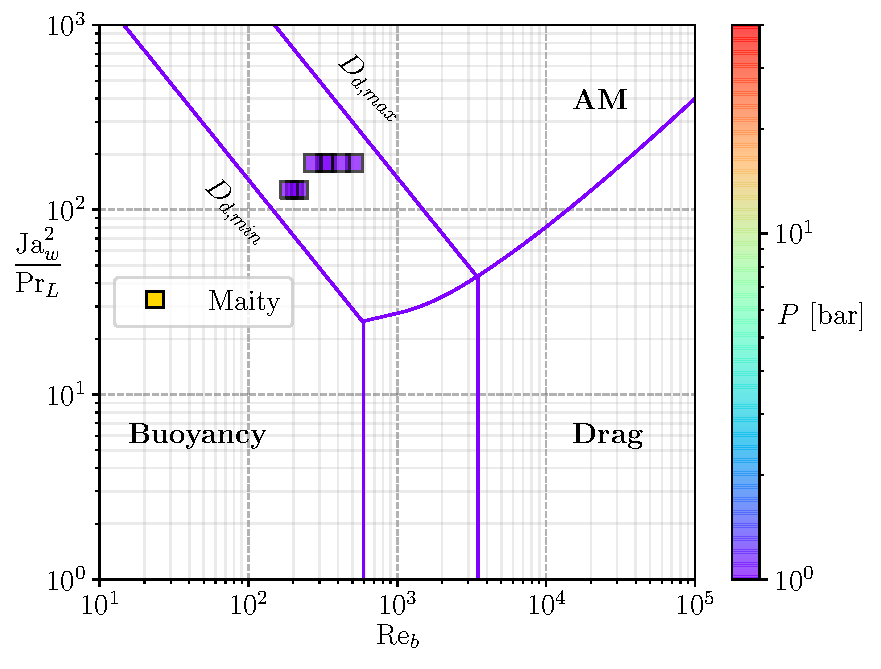
\includegraphics[width=0.45\linewidth]{img/bub_dyn/dep_maps/Maity_2.pdf}
\label{fig:exp_maity}
} 
\subfloat[Guan data]{
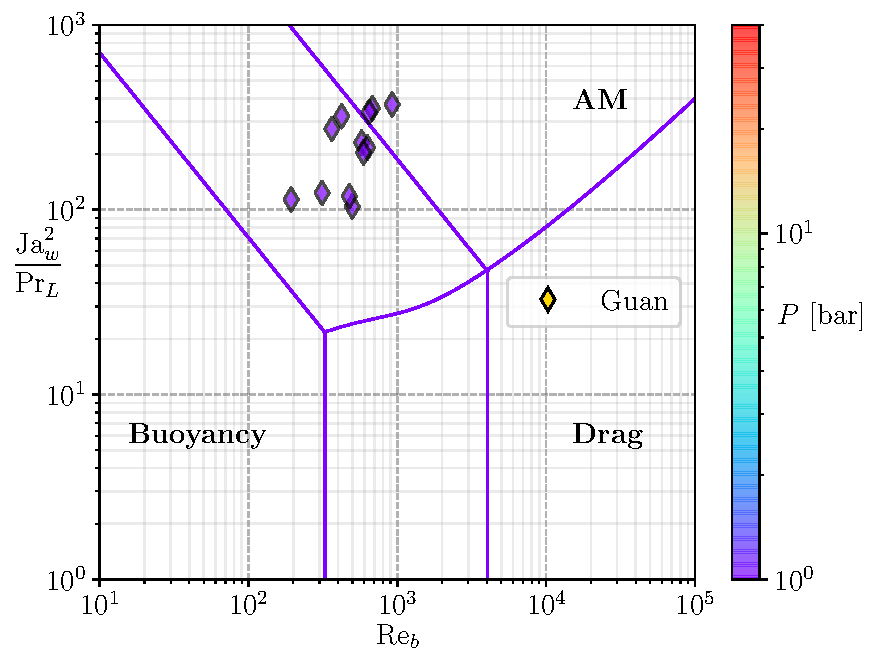
\includegraphics[width=0.45\linewidth]{img//bub_dyn/dep_maps/Guan_2.pdf}
\label{fig:exp_guan}
}
\\
\subfloat[Sugrue data]{
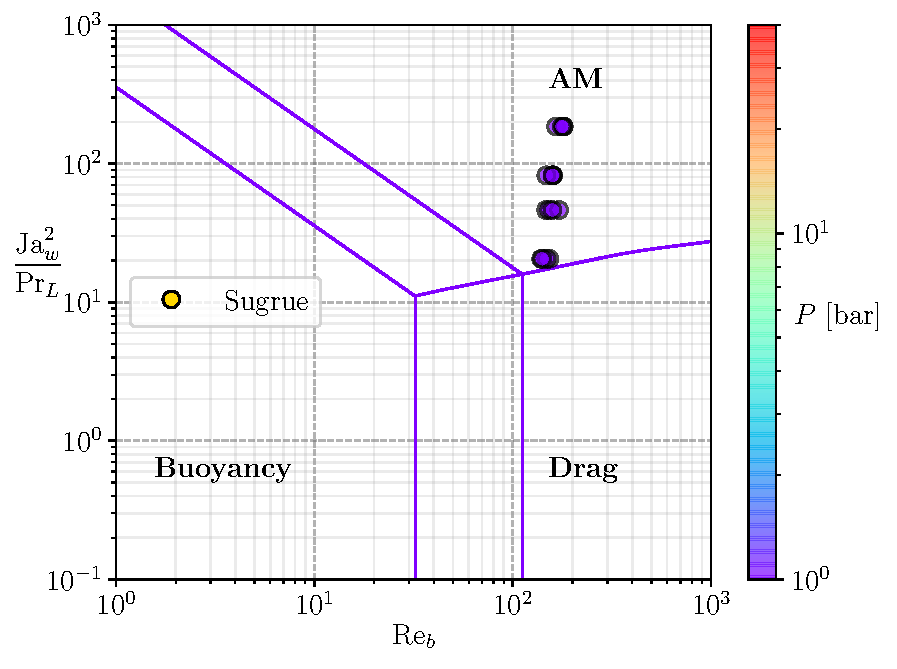
\includegraphics[width=0.45\linewidth]{img//bub_dyn/dep_maps/Sugrue_2.pdf}
\label{fig:exp_sugrue}
} 
\subfloat[Chen data]{
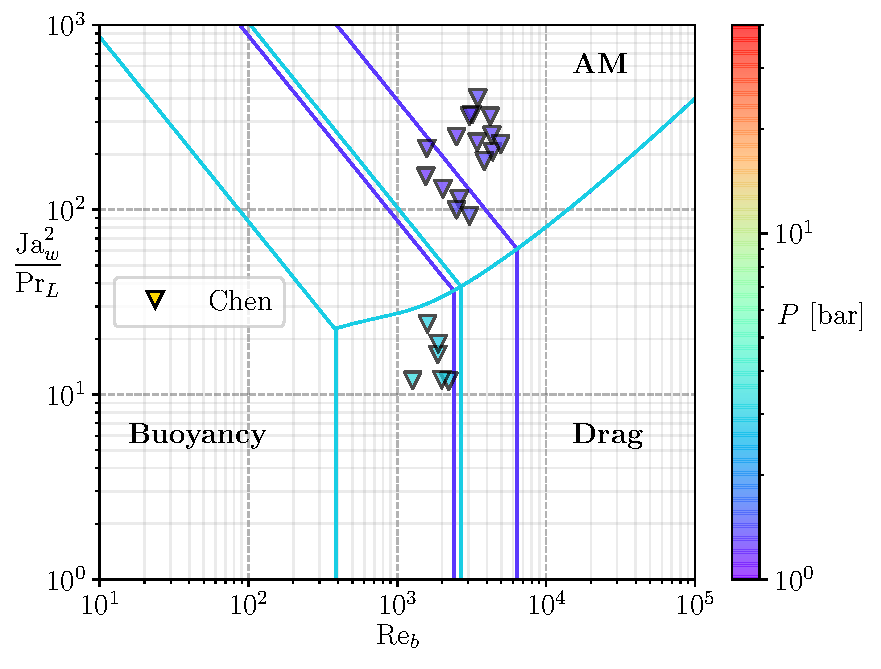
\includegraphics[width=0.45\linewidth]{img//bub_dyn/dep_maps/Chen_2.pdf}
\label{fig:exp_chen}
}
\\
\subfloat[Ren data]{
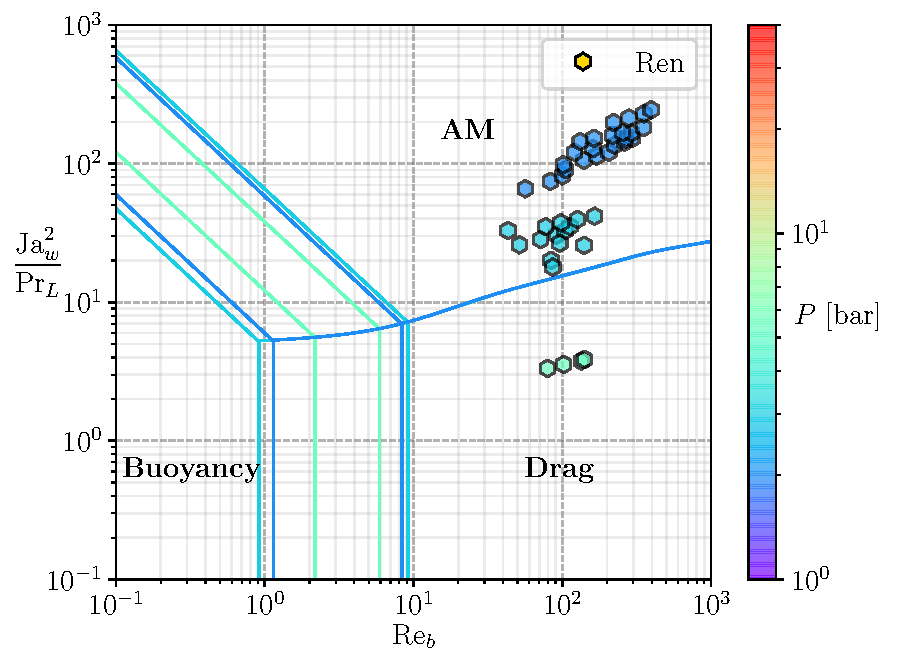
\includegraphics[width=0.45\linewidth]{img//bub_dyn/dep_maps/Ren_2.pdf}
\label{fig:exp_ren}
} 
\subfloat[Kossolapov data]{
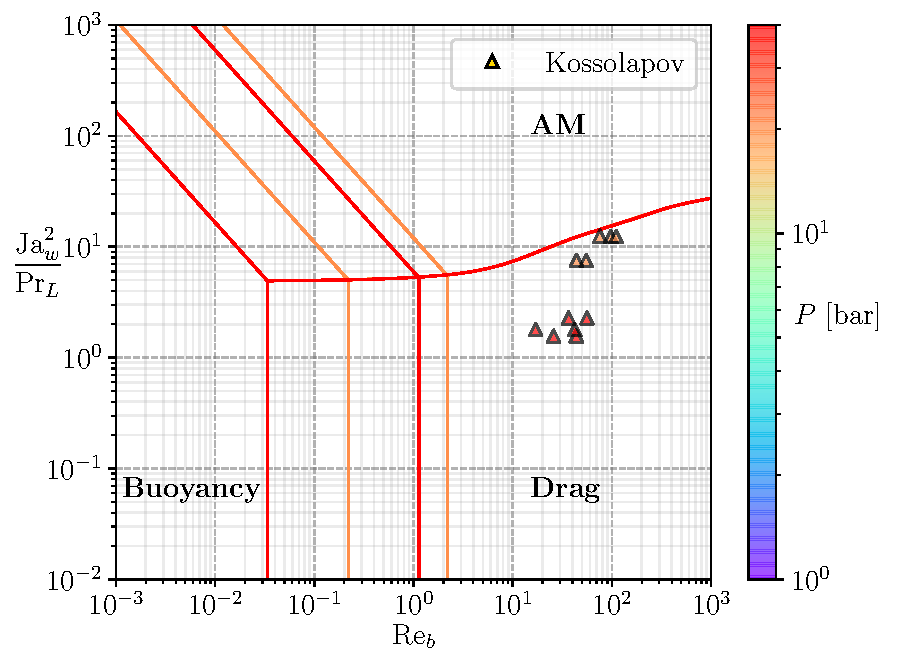
\includegraphics[width=0.45\linewidth]{img//bub_dyn/dep_maps/Kossolapov_2.pdf}
\label{fig:exp_koss}
}


	\caption{Regime maps for each water data sets from Table \ref{tab:exp_data}.}	
	\label{fig:exp_maps}
\end{center}
\end{figure}

\npar


When the pressure increases, we observe that the experimental measurements gradually move towards the drag dominant zone as seen on Figures \ref{fig:exp_ren} and \ref{fig:exp_koss}. This main difference in the dynamic regime when bubble departs by sliding arises from multiple effects:

\begin{itemize}
\item The decrease of $\rho_{L}/\rho_{V}$ with pressure, thus reducing $\Ja_{w}$ and the impact of the detaching added mass term ;
\item The higher liquid mass fluxes in Kossolapov experiments, increasing the impact of the drag ;
\item The decrease of $D_{d}$ with pressure, reducing the magnitude of buoyancy.
\end{itemize}

However, we see that some measurements lie close to the added mass / drag boundary (Figure \ref{fig:exp_koss}), indicating that the added mass force still plays a significant role for bubble detachment. This means that regardless of the operating pressure, the detaching term associated to the coupling between bubble growth and outer liquid flow should not be neglected in the force balance (Eq. \ref{eq:bdf_x_dep}).




\subsection{Departure Diameter Prediction}\label{subsec:Dd_pred}

\subsubsection{About the Use of Empiricism}
 
As previously mentioned, the case of bubble detachment in vertical flow boiling is particular since only one force maintains the bubble attached to its nucleation site: the capillary force (Eq.~\ref{eq:bdf_x_dep}). Its expression depends on the contact angle $\theta$, the angle half-hysteresis $\dtheta$ and the bubble foot radius $r_{w}$ (or ratio to bubble diameter $r_{w}/R$) and is thus very sensitive to those values. 

Paradoxically, those terms are among the least precisely known due to the difficulty of measurement and associated uncertainties. For instance, conducting precise evaluations of the contact angle near the bubble base through optical techniques can be challenging because of the strong temperature gradients close to the heated surface. 

\npar
Consequently, empirical choices have to be made in order to set a value to those parameters, often by relying on data-fitting or approximate measurements in other conditions. For instance, contact angles are often taken as arbitrary average values \cite{ren_development_2020} or measurements in room conditions \cite{sugrue_modified_2016} and applied over a whole set of experiments. This is questionable since contact angle is unlikely to remain unchanged over different operating conditions and surfaces with varying roughness and properties \cite{song_temperature_2021}.


\npar
However, no better information except those given by the authors can be used to evaluate the capillary force since no generic model exist to compute the contact angle and hysteresis. In this work, admitting a significant uncertainty (typically $5\degree$, as in Guan \cite{guan_bubble_2015}), we will use the following values for the contact angles :


\begin{itemize}
\item $\theta_{u}=25.3\degree$ and $\theta_{d} = 6.6\degree$ for Thorncroft data (measured values for FC-87 on nichrome \cite{thorncroft_bubble_2001}) ;
\item $\theta_{u} = 50\degree$ and $\theta_{d} = 40\degree$ for Maity data (measured average contact angles for each bubble during its lifetime \cite{maity_effect_2000}) ;
\item $\theta_{u} = 130\degree$ and $\theta_{d} = 65\degree$ for Chen data (chosen values in their study following measurements for water on stainless steel at high temperature by Kandlikar \etal \cite{kandlikar_contact_2002}) ;
\item $\theta_{u}=91\degree$ and $\theta_{d} = 8\degree$ for Sugrue data (measured values at room temperature \cite{sugrue_effects_2012}) ;
\item $\theta_{u} = 75\degree$ and $\theta_{d} = 30\degree$ for Guan data (measured average value through experimental visualizations \cite{guan_bubble_2015}) ;
\item $\theta_{u} = 45\degree$ and $\theta_{d} = 36\degree$ for Ren data (chosen values in their study \cite{ren_development_2020}) ;
\item $\theta = 80 \degree$ for Kossolapov data (typical contact angle for water on ITO \cite{kossolapov_experimental_2021}) and $\dtheta=1\degree$ assuming that the very small bubbles at high pressure are nearly not tilted.
\end{itemize}


Similarly, the bubble foot radius $r_{w}$ is often empirically assumed to be either constant \cite{klausner_vapor_1993} proportional to the bubble radius \cite{sugrue_modified_2016, mazzocco_reassessed_2018} or to follow a linear or logarithmic law of $R$ \cite{zhou_experimental_2020, guan_bubble_2015}. That is why we chose to use the truncated sphere hypothesis (Eq. \ref{eq:rw}) to compute $r_{w}$ using $R$ and $\theta$.

Finally, we would like to acknowledge that the empiricism to evaluate those parameters represents one of the biggest flaws of the force-balance approach. Indeed, such a model aims to detect small sign changes in a sum of a few $\mu\mathrm{N}$ of forces that are decades larger as pointed out by Bucci \etal \cite{bucci_not-so-subtle_2021}. Mechanistic models are thus strongly sensitive to any extra parameter included in the modeling of the forces.

\subsubsection{Growth Constant Value}

As discussed in Section \ref{sec:bub_growth}, the growth constant $K$ with a value close to one or lower usually provides reasonable approximation of the bubble radius. In particular, subcooled flow boiling may need smaller values of $K$, as well as fluids with high Prandtl numbers. 

\npar

To avoid a systematic overestimation of the added mass term which could lead to strong underestimations of the departure diameter in cases that would present strong subcoolings, liquid velocity or working fluids with low thermal conductivity, we will use:

\begin{equation}
K=\frac{2b}{\sqrt{\pi}},\ b=0.24
\end{equation}
as proposed by Yoo \etal \cite{yoo_development_2018} to model the superheated liquid diffusion growth term.


\subsubsection{Predictions}

We consider the non-dimensional force balance before departure.

\begin{equation}
C_{AM,x}K^{2} \frac{\Ja_{w}^{2}}{\Pr_{L}} + \frac{1}{3}\frac{\Re_{b}}{\Fr} + \frac{1}{8}C_{D}\Re_{b} = \frac{1}{2} \frac{f_{C,x}}{\Ca}
\end{equation}

Since we only have the capillary term hindering departure as a first approach, we can suppose that departure is reached when:

\begin{equation}
C_{AM,x}K^{2} \frac{\Ja_{w}^{2}}{\Pr_{L}} + \frac{1}{3}\frac{\Re_{b}}{\Fr} + \frac{1}{8}C_{D}\Re_{b} > \frac{1}{2} \frac{f_{C,x}}{\Ca}
\label{eq:pred_nogr}
\end{equation}
which is similar to considering that the other forces overcome the capillary force.


\npar
On Figure \ref{fig:pred_nosensi}, we show the predictions obtained with the proposed modeling and those obtained with Mazzocco's recent model \cite{mazzocco_reassessed_2018}. 


\begin{figure}[h!]
\centering
\subfloat[Proposed model without accounting for contact angle uncertainties]{
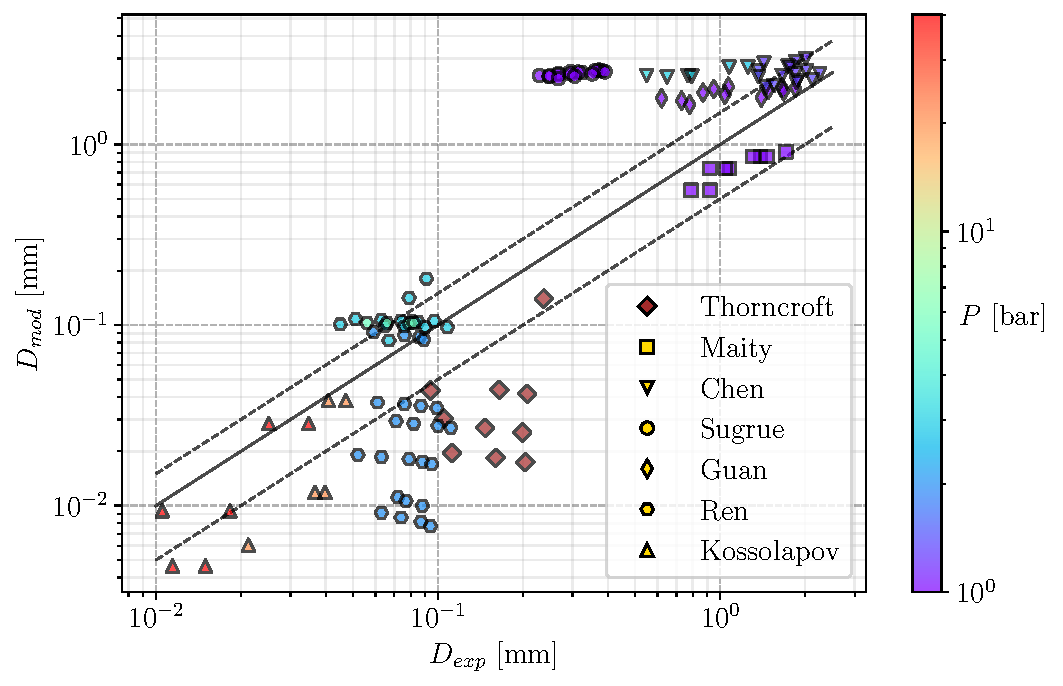
\includegraphics[width=0.6\textwidth]{img/bub_dyn/pred_nosensi.pdf}
}
\\
\subfloat[Mazzocco model]{
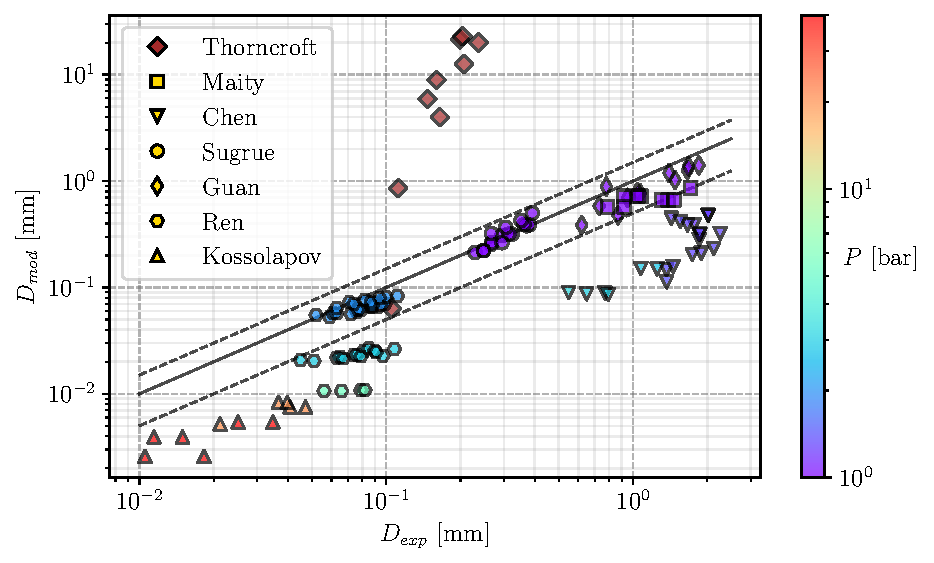
\includegraphics[width=0.6\textwidth]{img/bub_dyn/pred_mazzocco.pdf}
}

\caption{Predicted bubble departure diameters. $\pm 50\%$ error bars are indicated.}
\label{fig:pred_nosensi}
\end{figure}

\npar


The model have an acceptable trend on some experimental sets, but strong overestimation occur on the cases of Sugrue. Moreover, we observe significant underestimations on the data of Ren at 2 bar and Thorncroft.

Mazzocco's model provides a good accuracy on the data of Sugrue, Guan, Maity and Ren (2 bar). However, we observe very large overestimation over Thorncroft's measurements and significant underestimation on Chen, Ren (3 and 5 bar) and Kossolapov measurements. 



\subsection{Discussion and accounting for parameters uncertainties}


The aforementioned errors observed for the proposed model may originate from various reasons:

\begin{itemize}
\item The contact angle proposed for Sugrue cases is high with a large hysteresis, suggesting strongly deformed and flattened bubbles under the truncated sphere hypothesis. Based on images from Sugrue's work \cite{sugrue_experimental_2014}, a comparison between a real bubble with the assumed shape is presented on Figure \ref{fig:bubshape_sugrue}. This shows a huge difference which indicates that the contact angle and hysteresis values may be overestimated. Using the available images, the ratio of the bubble diameter to the apparent bubble foot would lead to an average contact angle $\theta \approx 20\degree$ for a truncated sphere. Noting that a larger inclination is observed for the bubbles under higher mass fluxes leads us to suppose a value $\dtheta \approx 15\degree$. This represent a similar inclination to contact angle ratio ($\dtheta / \theta$) compared to the initially proposed values. The resulting new shape is also presented on Figure \ref{fig:bubshape_sugrue} and seem to better represent the actual bubble.




\begin{figure}[h!]
\centering
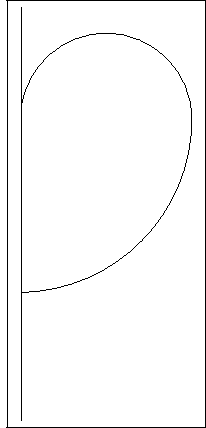
\includegraphics[height=0.4\linewidth]{img/bub_dyn/bub_sugrue.pdf}
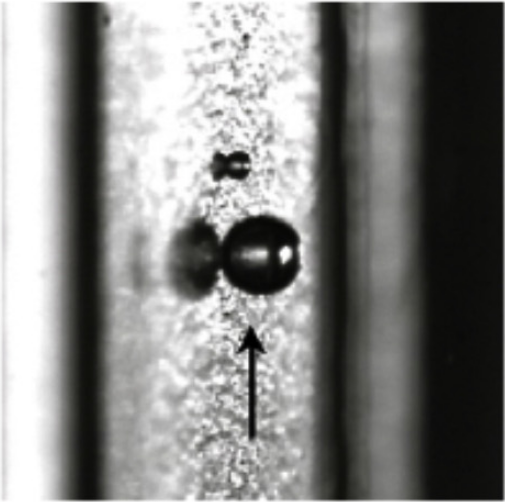
\includegraphics[width=0.45\linewidth]{img/bub_dyn/pic_sugrue.png}
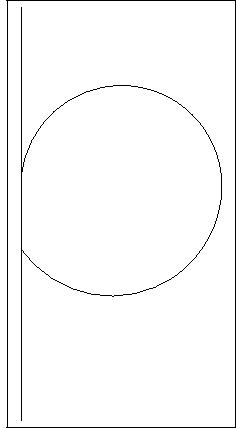
\includegraphics[height=0.4\linewidth]{img/bub_dyn/newbub_sugrue.pdf}
\caption{Initially assumed, real and reassessed bubble shape for Sugrue cases (picture adapted from \cite{sugrue_experimental_2014}).}
\label{fig:bubshape_sugrue}
\end{figure}


\item For cases where limited under and overestimation is observed, we may allow to account for an uncertainty as high as $5 \degree$ for the average contact angle $\theta$ and half-hysteresis $\dtheta$.

\item As mentioned earlier, applying the same contact angle and hysteresis over a wide range of measurements is a strong assumption, especially for cases where different pressures and bubble diameter variations are observed. Thus, we may slightly distinguish the applied values of $\theta$ and $\dtheta$ for different pressures within a given experiment, keeping a change no larger than $5 \degree$.

\item Kossolapov cases at $G_{L}=500~\debm$ are better predicted. Cases under higher mass fluxes ($1000$ and $1500~\debm$) present underestimation that could come from the value of $\dtheta$. At such mass fluxes, the Weber number can be up to a decade higher and bubbles may thus accept a larger inclination before detachment.

\item Cases of Ren and Chen rely on chosen values for $\theta$ and $\dtheta$ and not on measured ones. They are therefore subject to strong uncertainties. We can note that the values for Chen cases are significantly high.

\item The proposed growth law is still rather simple and may miss significant information, especially regarding bubble size and fluid properties such as the Prandtl number.

\item Errors on Thorncroft cases may be linked to uncertainties regarding FC-87 properties. Indeed, we use the values given at $T_{sat}=29\degree$ at 1 bar in his work \cite{thorncroft_experimental_1998}. However, the saturation temperature indicated in his test matrix is close to $40\degree$ which means that measurements were conducted at a higher pressure, for which we do not have FC-87 properties.


\end{itemize}





Therefore, using modified values of $\theta$ and $\dtheta$ among experimental data sets with no more than a $5 \degree$ change (except for Sugrue cases reassessed values) leads to predictions on Figure \ref{fig:pred_sensi}.






\begin{figure}[h!]

\subfloat[Modified contact angle and hysteresis values.]
{
\scriptsize
\centering
\begin{tabular}[b]{p{30mm}|c c } 
Author & $\theta$ [$\degree$] & $\dtheta$ [$\degree$]\\
\hline
\\
Thorncroft & 21 & 14 \\
\\
Maity & 45 & 10  \\
\\
Chen & 92.5 & 27.5 \\
\\
Sugrue & 20 & 15 \\
\\
Guan & 47.5 & 17.5 \\
\\
Ren (2 bar) & 45.5 & 7.5 \\
\\
Ren (3 bar) & 37.5 & 3.5 \\
\\
Ren (5 bar) & 35.5 & 3.5 \\
\\
Koss. (500$~\debm$) & 80 & 0.5 \\
\\
Koss. (1000$~\debm$) & 80 & 1 \\
\\
Koss. (1500$~\debm$) & 80 & 1.5 \\
\\
\hline
\end{tabular}

\label{tab:angle_sensi}
}
\subfloat[Predicted bubble departure diameters.]{
\centering
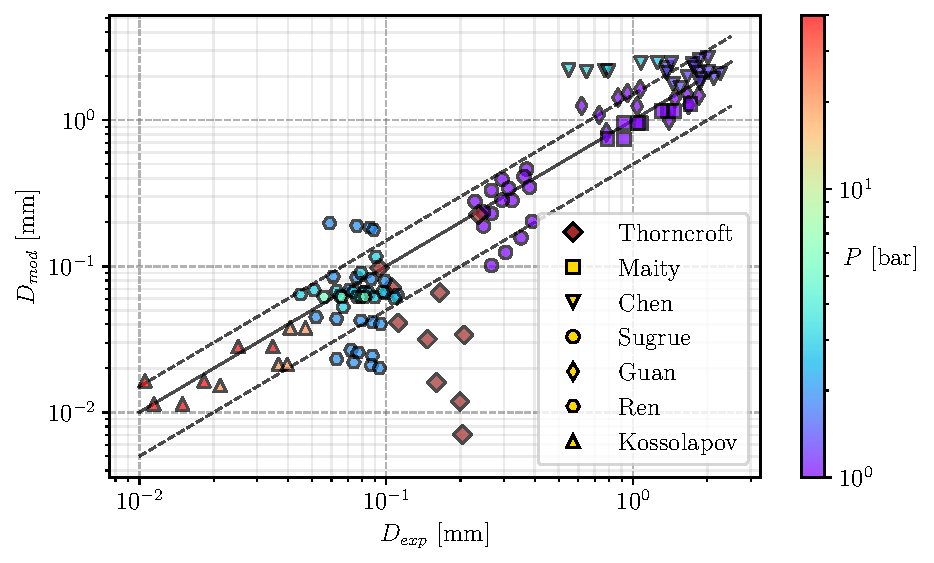
\includegraphics[width=0.6\textwidth]{img/bub_dyn/pred_sensi.pdf}
}

\caption{Proposed model performance while accounting for contact angle uncertainties}
\label{fig:pred_sensi}
\end{figure}

\npar


The predictive capacity of the model is significantly enhanced, especially on Sugrue's cases which tends to indicate that the contact angle reassessment was justified under the truncated sphere hypothesis. Table \ref{tab:mod_errors} summarizes the average errors obtained with the present model and Mazzoco's one.

\npar

The proposed model achieves an overall better predictive capability even when excluding measurements from Thorncroft on which Mazzocco's model strongly overestimates the departure diameter. Mazzocco's model is still better on Sugrue and Guan cases since it was built and validated using those measurements. It better predicts results from Ren but only for the 2 bar cases while it underestimates the departure diameter for higher pressures. Those results are a coupled effect of his optimized growth law along with the imposed value of $r_{w}/R$ and the use of the inclination angle to hinder departure as mentioned in \ref{subsec:AM}.


\begin{table}[h!]

\scriptsize
\centering
\begin{tabular}[b]{p{30mm}|c c } 
Author & Mazzocco & Present model\\
\hline
\\
Thorncroft & 4874\% & 46.2\% \\
\\
Maity & 39.7\% & 13.8\%  \\
\\
Chen & 83.8\% & 73.6\% \\
\\
Sugrue & 9.73\% & 21\% \\
\\
Guan & 25.5\% & 44.5\% \\
\\
Ren & 40.32\% & 47\% \\
\\
Kossolapov & 78.3\% & 24.2\% \\
\\
Total \newline (without Thorncroft) & {46.58\%} & {43.3\%}\\
\hline
\end{tabular}
\caption{Average relative error reached by the models.}
\label{tab:mod_errors}
\end{table}

\npar


The approach demonstrated the importance and the strong influence of the contact angle and hysteresis. A small change of their value (staying in the uncertainty range of $5\degree$) allowed to reach reasonable predictions over a large range of bubble departure diameters with the proposed model, using a reduced number of empirical parameters.


\section{Sliding phase}\label{sliding}


\subsection{Modeling}

After departure, bubbles slide over a distance $l_{sl}$ which scales the impact of the sliding phenomenon over the wall heat transfer. Achieving good prediction of bubble sliding velocity is then important if one wishes to correctly quantify its impact. Following the force balance framework presented in Section \ref{sec:bub_forces}, we can write Newton's second law parallel to the wall for the sliding bubble.


\begin{align}
\nonumber \rho_{V}\derive{\parth{V_{b}U_{b}}}{t} =& - \pi R\sigma f_{C,x}+ \frac{4}{3}\pi R^{3}\parth{\rho_{L}-\rho_{V}}g + \frac{1}{2}C_{D}\rho_{L}\pi R^{2} U_{L}^{2} \\
%
&+ \frac{4}{3}\pi R^{3}\rho_{L}\crocht{3C_{AM,x}\frac{\dot{R}}{R}U_{rel} - C_{AM,x}\derive{U_{b}}{t}}
\end{align}

This equation can be re-written to express the bubble acceleration.

\begin{align}
\nonumber \parth{1+\frac{\rho_{L}}{\rho_{V}}C_{AM,x}}\derive{U_{b}}{t} = & \parth{\frac{\rho_{L}}{\rho_{V}}-1}g + \frac{3}{8}\frac{C_{D}}{R}\frac{\rho_{L}}{\rho_{V}}\parth{U_{L}-U_{b}}\bars{U_{L}-U_{b}} \\
%
&+ 3\frac{\dot{R}}{R}\crocht{C_{AM,x}\frac{\rho_{L}}{\rho_{V}}\parth{U_{L}-U_{b}}-U_{b}} - \frac{3}{4}\frac{\sigma}{\rho_{V}}\frac{f_{C,x}}{R^{2}}
\label{eq:ub_dot}
\end{align}

Then, we numerically solve this equation from the moment when $R\geq R_{d}$ using a first order Euler scheme for a duration close to the experimental sliding time. To assess the validity of Eq \ref{eq:ub_dot}, we modify the growth constant $K$ in order to roughly match experimental radius measurements. The goal is to verify if the force balance allows a good prediction of bubble velocity provided a correct bubble growth.  Next sections compare obtained results against low and high pressure data.

\subsection{Low Pressure Sliding}

Maity \cite{maity_effect_2000} provided simultaneous measurements of bubble radius and velocity over time in vertical boiling for three liquid mass fluxes near saturation conditions. The contact angles were kept the same as in \ref{subsec:Dd_pred} since Maity provided average values over the bubble lifetime.

\npar

Results are displayed on Figure \ref{fig:slide_maity}. The model seems to fairly good predict bubble sliding velocity for the 3 cases. The moment of departure is a bit underestimated as previously observed (Figure \ref{fig:pred_nosensi}).

\begin{figure}[h!]
\begin{center}
\subfloat[$\Delta T_{w}=5.0$\degree C, $G_{L}=73.8~\debm$]{
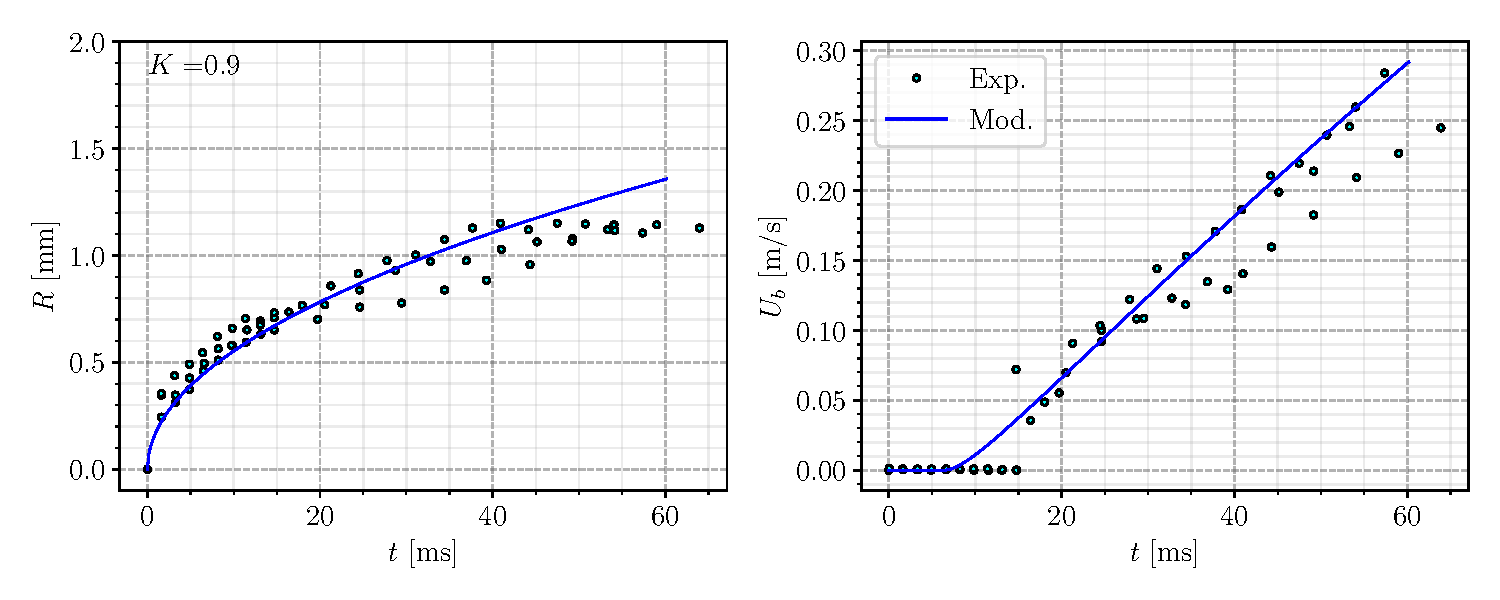
\includegraphics[width=0.85\linewidth]{img/bub_dyn/sliding/maity_V0p077.pdf}
} 
\\
\subfloat[$\Delta T_{w}=5.9$\degree C, $G_{L}=143.8~\debm$]{
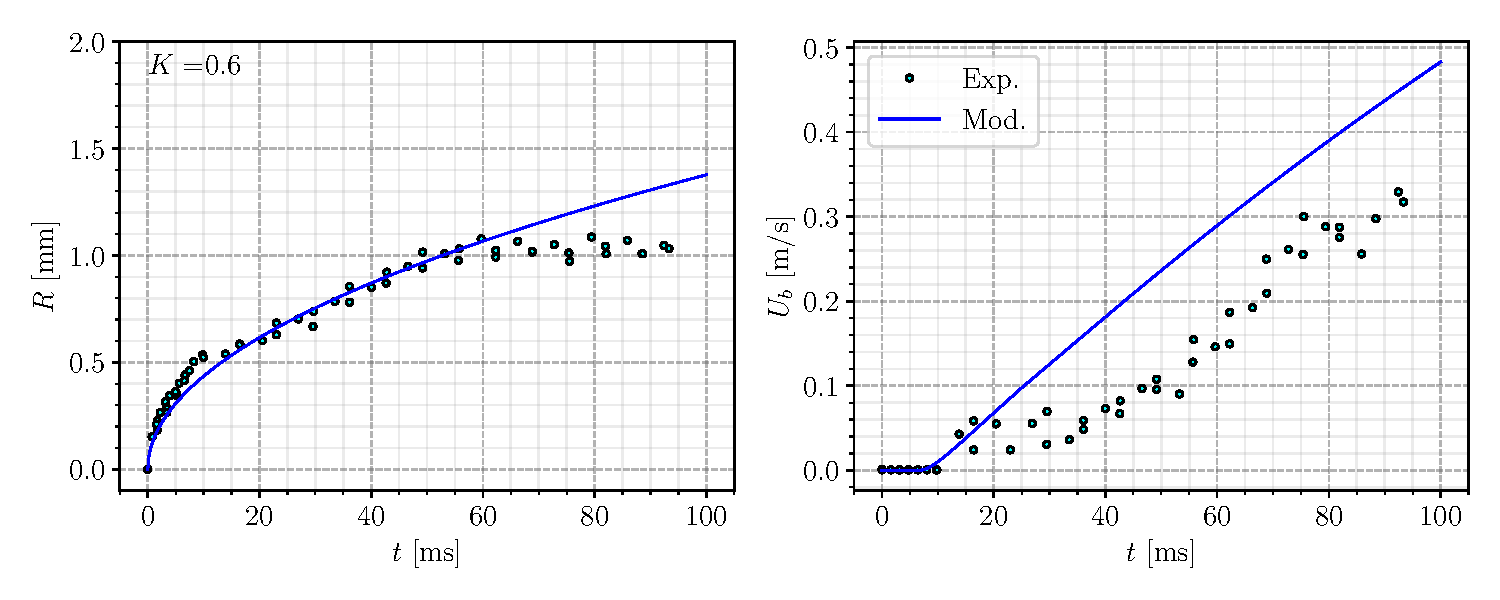
\includegraphics[width=0.85\linewidth]{img/bub_dyn/sliding/maity_V0p15.pdf}
}
\\
\subfloat[$\Delta T_{w}=5.9$\degree C, $G_{L}=239.6~\debm$]{
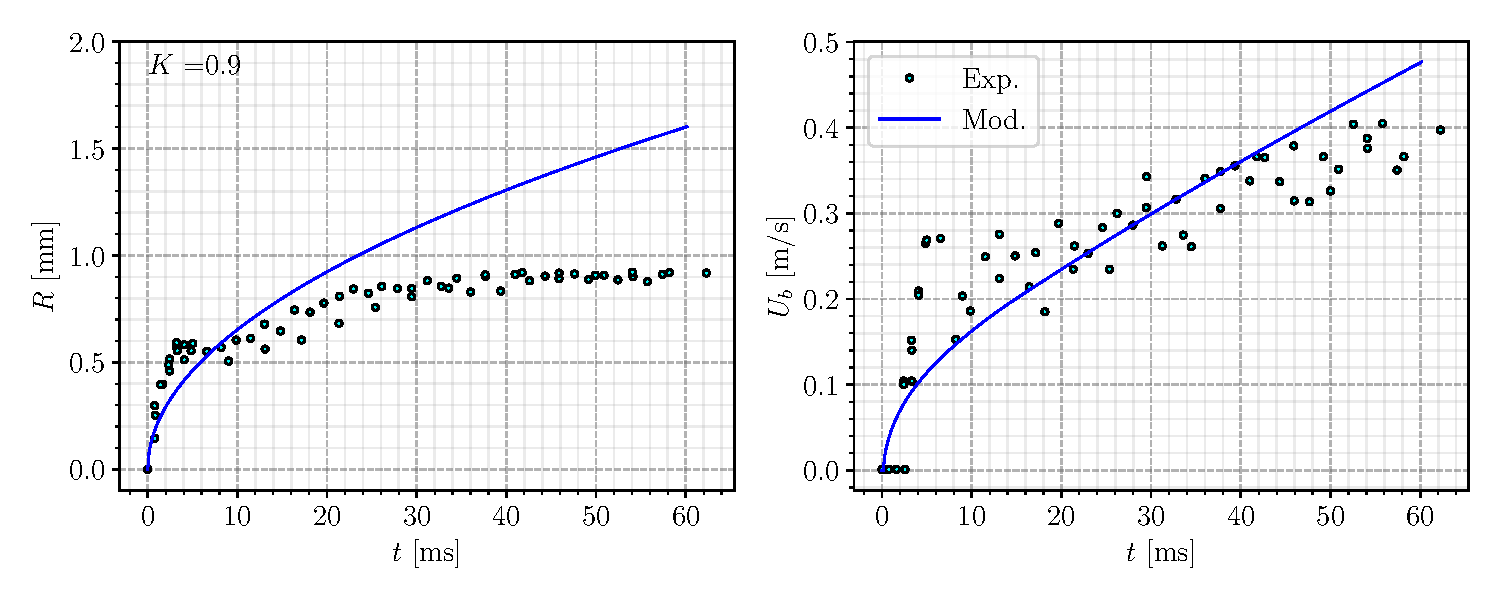
\includegraphics[width=0.85\linewidth]{img/bub_dyn/sliding/maity_V0p25.pdf}
}
	\caption{Bubble sliding velocity predictions on Maity cases}
	\label{fig:slide_maity}
\end{center}
\end{figure}

\npar

The biggest discrepancy is observed for the case at $G_{L}=143.8~ \debm$. The slope of the velocity profile is close to the experiments, but the bubble reaches a nearly constant acceleration too rapidly which yields an approximately constant overestimation of $0.1$~m/s.

\npar

The $G_{L}=239.6~ \debm$ is well predicted regarding the velocity. However, the growth profile was difficult to match since measurements exhibit significant changes in growth regime after departure, which is probably due to the bubble being large enough to be impacted by the bulk flow. We can note that values of $K$ between 0.5 and 1 were used to better fit the bubble radius time profile.

\npar

Regarding the relative velocity between the bubble and the surrounding liquid, the ratio $\dfrac{U_{b}}{U_{L}}$ greatly overcomes 1 which means the bubble slides much faster than the liquid. This is a consequence of both the low values of $G_{L}$ along with the large bubble sizes inducing a great acceleration by the buoyancy force.






\subsection{High Pressure Sliding}

In his work, Kossolapov \cite{kossolapov_experimental_2021} conducted measurements of radius and sliding length over thousands of individual bubbles and then provided the associated statistical distributions. To compare our model with his measurements, we took the upper and lower bounds of $R$ and $l_{sl}$ over time and plotted the associated bands of measured values as shown on Figure \ref{fig:slide_koss_20bar} and \ref{fig:slide_koss_40bar}.


\begin{figure}[h!]
\begin{center}
\subfloat[$\phi_{w}=0.178$~MW/m\up{2}, $\Delta T_{w}=12.6$K, $G_{L}=500~\debm$]{
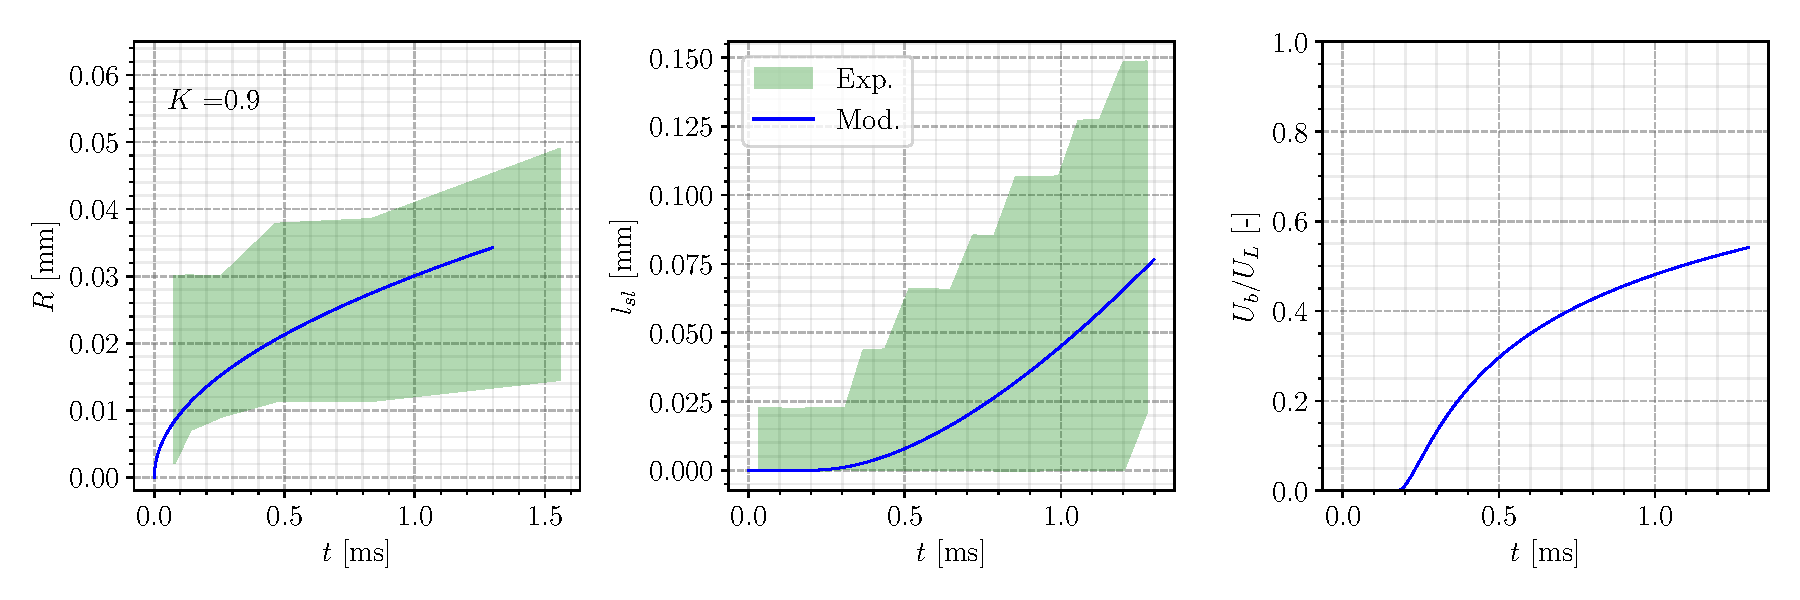
\includegraphics[width=0.85\linewidth]{img/bub_dyn/sliding/Koss_P20_G500.pdf}
} 
\\
\subfloat[$\phi_{w}=0.495$~MW/m\up{2}, $\Delta T_{w}=16.1$K, $G_{L}=994~\debm$]{
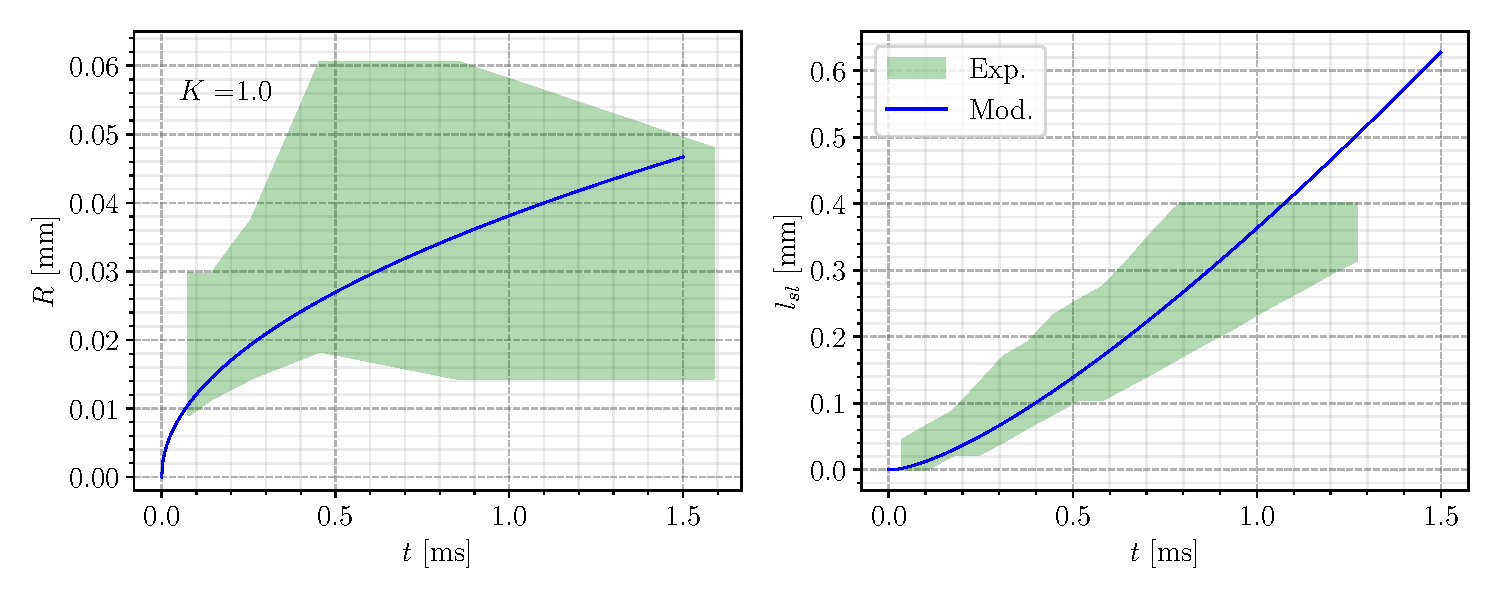
\includegraphics[width=0.85\linewidth]{img/bub_dyn/sliding/Koss_P20_G1000.pdf}
} 
\\
\subfloat[$\phi_{w}=0.487$~MW/m\up{2}, $\Delta T_{w}=16.2$K, $G_{L}=1504~\debm$]{
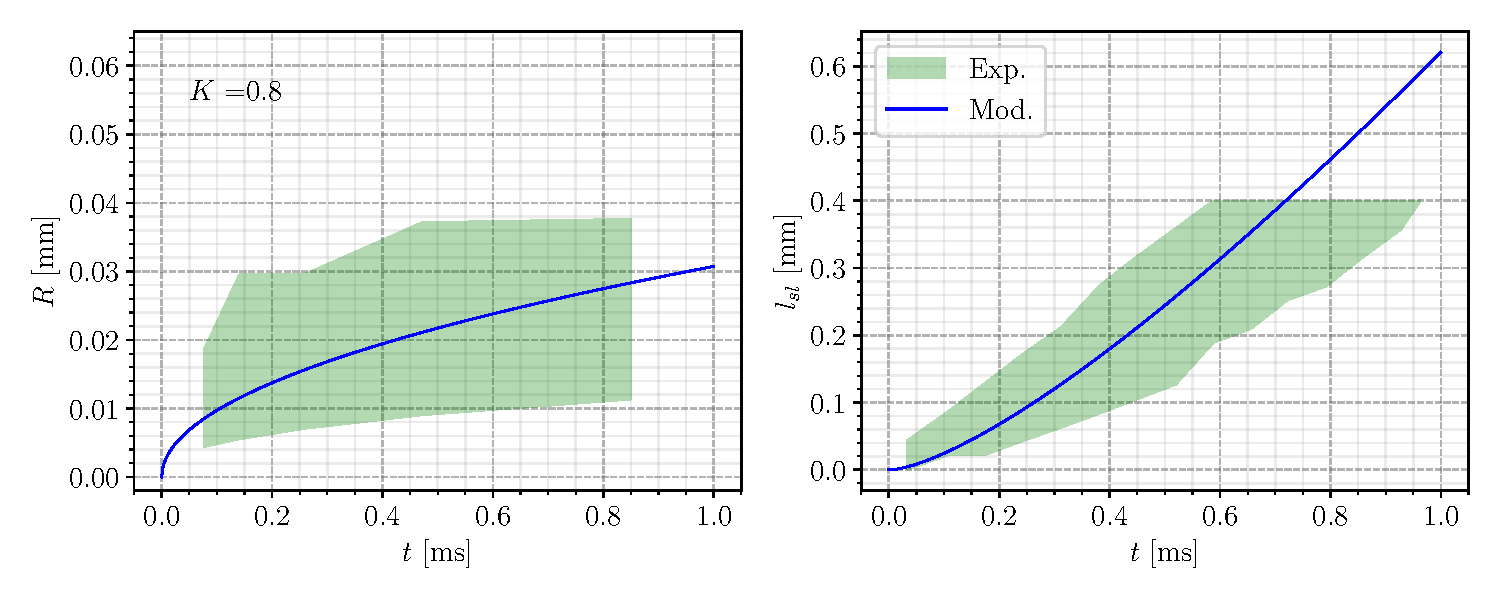
\includegraphics[width=0.85\linewidth]{img/bub_dyn/sliding/Koss_P20_G1500.pdf}
} 
	\caption{Bubble sliding length predictions on Kossolapov cases - $P=20$ bar}
	\label{fig:slide_koss_20bar}	
\end{center}
\end{figure}



\begin{figure}[h!]
\begin{center}
\subfloat[$\phi_{w}=0.291$~MW/m\up{2}, $\Delta T_{w}=10.1$K, $G_{L}=500~\debm$]{
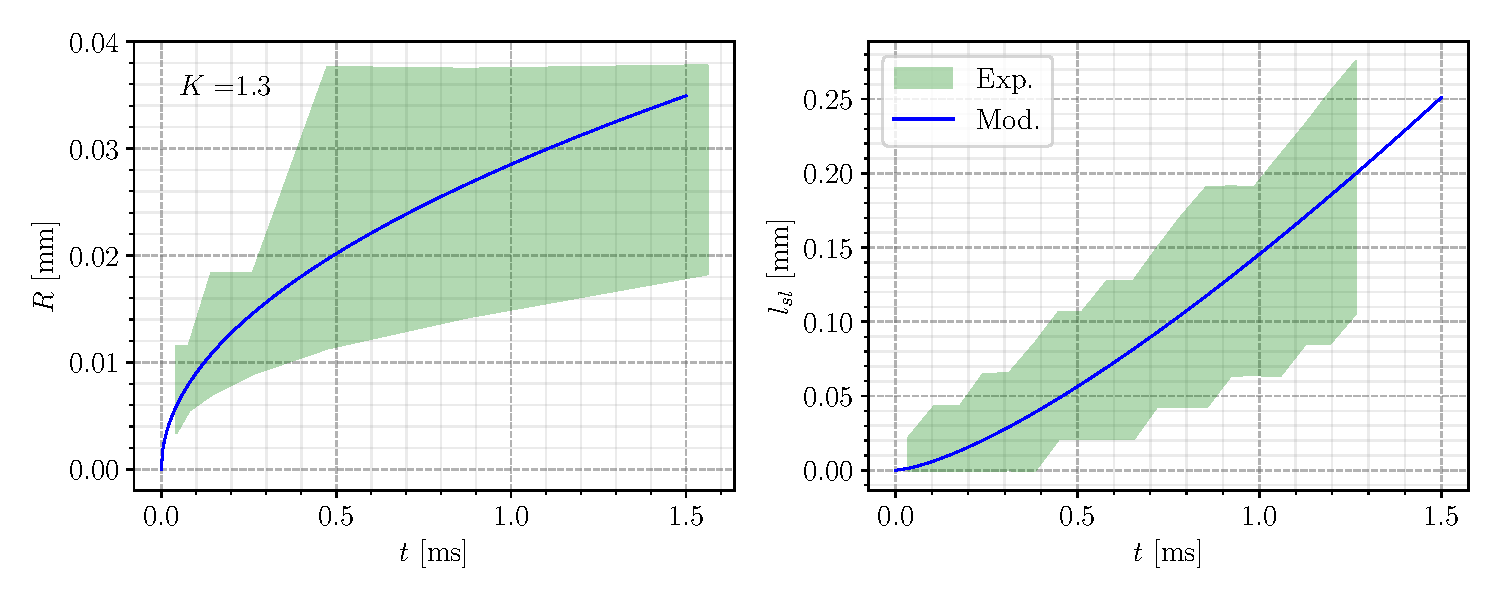
\includegraphics[width=0.85\linewidth]{img/bub_dyn/sliding/Koss_P40_G500.pdf}
} 
\\
\subfloat[$\phi_{w}=0.361$~MW/m\up{2}, $\Delta T_{w}=10.8$K, $G_{L}=994~\debm$]{
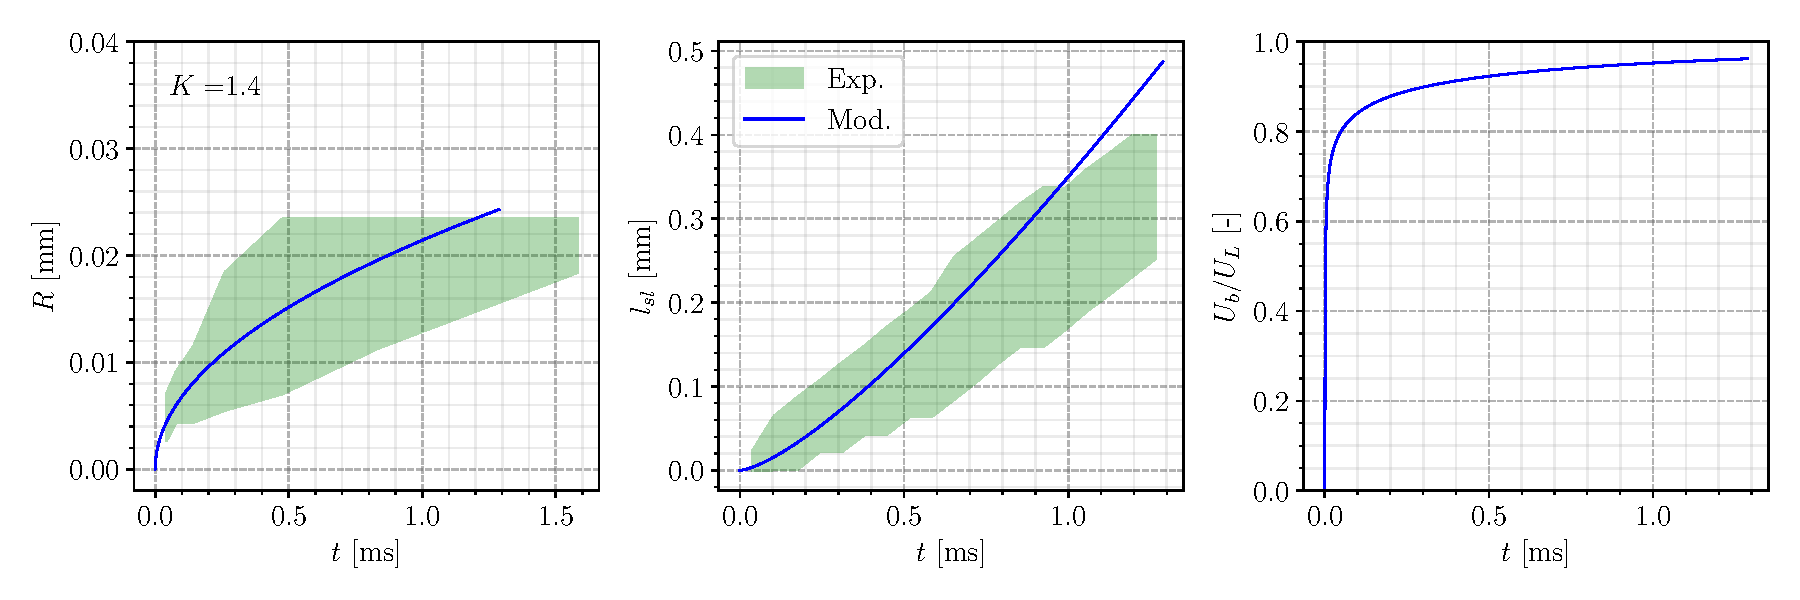
\includegraphics[width=0.85\linewidth]{img/bub_dyn/sliding/Koss_P40_G1000.pdf}
} 
\\
\subfloat[$\phi_{w}=0.613$~MW/m\up{2}, $\Delta T_{w}=12.2$K, $G_{L}=1504~\debm$]{
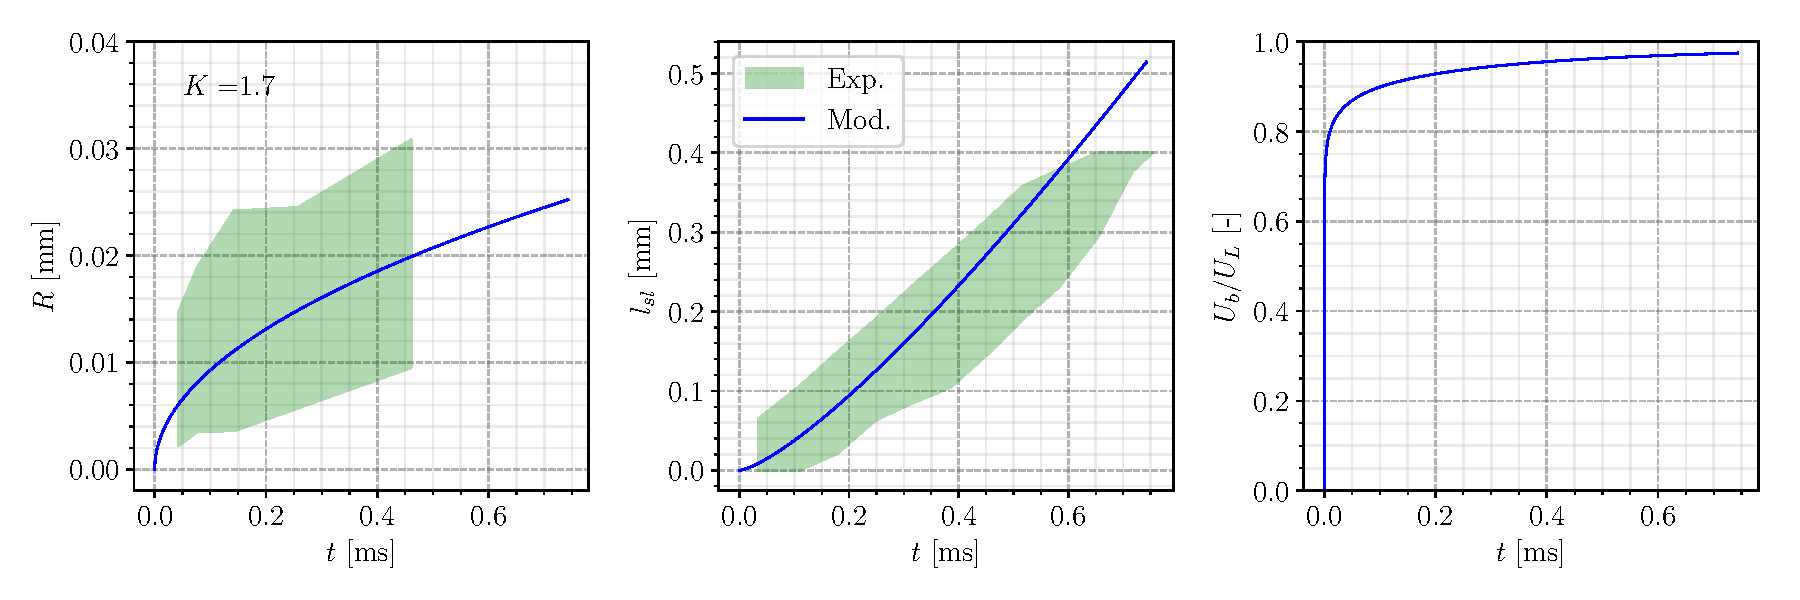
\includegraphics[width=0.85\linewidth]{img/bub_dyn/sliding/Koss_P40_G1500.pdf}
} 
	\caption{Bubble sliding length predictions on Kossolapov cases - $P=40$ bar}	
	\label{fig:slide_koss_40bar}
\end{center}
\end{figure}



Comparisons were done for cases at 20 bar and 40 bar and 3 different values of $G_{L}$. The value of $\dtheta$ for the simulations was kept really small ($2 \degree$ at 20 bar and $0.5\degree$ at 40 bar) since bubble tilt is supposed to reduce during sliding because the relative velocity regarding the liquid flow is diminishing. Moreover, higher pressure means smaller bubbles that are even more unlikely to present a significant contact angle hysteresis. We also want to mention that neglecting the capillary term in Eq.~\ref{eq:ub_dot} had a minor impact over the results except that the bubble accelerates a little bit faster. 

\npar
The obtained results are in good agreement with the sliding length profile vs. time, which means bubble sliding velocity is well predicted for those cases. Values of $K$ between 0.8 and 2 were needed to match the bubble radius measurements.

\npar

We see that bubbles are rapidly reaching sliding velocities between 80\% and 95\% of the local liquid velocity. Only the 20 bar case at $G_{L}=500\debm$ where the bubble departs slightly later, reaching approximately 55\% of the liquid velocity.


\subsection{Comparison of Forces in Sliding Stage}

In order to identify the main accelerating forces, we compare the amplitude of the forces during the sliding phase for one low pressure case of Maity and one high pressure case of Kossolapov (Figure \ref{fig:forces_sliding}).


\begin{figure}[h!]
\begin{center}
\subfloat[Maity : $\Delta T_{w}=5.9 \degree$ C, $G_{L}=239.6~\debm$]{
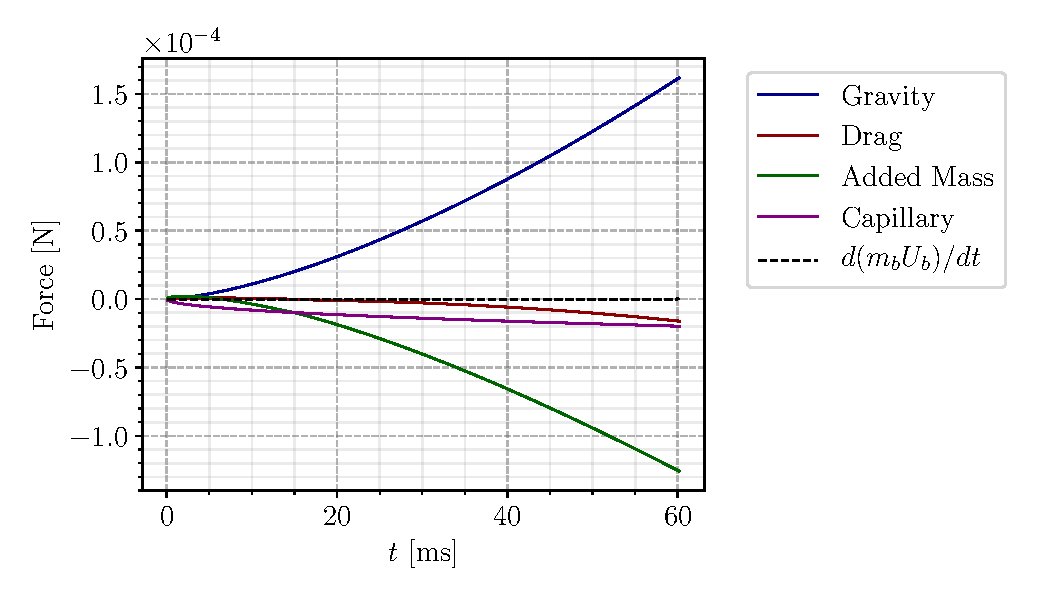
\includegraphics[width=0.5\linewidth]{img/bub_dyn/sliding/maity_V0p25_forces.pdf}
} 
\subfloat[Kossolapov : $P=40$ bar, $\phi_{w}=0.613$~MW/m\up{2}, $G_{L}=1504~\debm$]{
\includegraphics[width=0.5\linewidth]{img/bub_dyn/sliding/Koss_P40_G1500_forces.pdf}
} 
	\caption{Amplitude of each force during sliding}	
	\label{fig:forces_sliding}
\end{center}
\end{figure}


\npar


It appears that at high pressure and liquid velocity, the drag force is the main driving force and stays positive since the bubble do not slide faster than the rapid surrounding liquid (reaching approximately 80\% of the local liquid velocity). On the other hand, larger bubbles observed at low pressure and liquid velocity are accelerated by buoyancy due to their larger volume, with a nearly negligible Drag force. In both cases, the added mass force can not be neglected especially when bubble velocity rises by limiting its acceleration induced by the larger force (buoyancy or drag in the presented cases). This further emphasizes the importance of a proper derivation of the added mass force regardless of the boiling conditions. The capillary force seem to be a limited but constant slowing term in both cases. Finally, the amplitude of the forces involved can span from roughly $10\times 10^{-4}$ N at low pressure (much greater than the rate of change of bubble momentum laying around $10^{-9}$ N) down to a few nN at higher pressure (same order of magnitude as the rate of change of bubble momentum), especially due to the bubble size.

\npar

This comparison highlights the fact that the proposed model is able to represent different forces hierarchy depending on the flow conditions and to acceptably predict the associated bubble sliding velocity, which is an encouraging point regarding its generality.


\clearpage

\section{Bubble Lift-Off}

The question of lift-off for a single bubble in vertical boiling is trickier than for horizontal boiling. Indeed, in horizontal boiling, lift-off is ensured thanks to the buoyancy force that will continuously increase as the bubble grows. It can also be promoted by the lift force if the bubble slides slower than the liquid. This facilitates the identification of the moment when bubble leaves the surface (Figure \ref{fig:exp_lift_hor_maity}).

\begin{figure}[h!]
\centering
\includegraphics[width=0.7\linewidth]{img/bub_dyn/lift-off/lift_exp_hor_maity.PNG}
\caption{Visualization of bubble lift-off in horizontal boiling conducted by and adapted from Maity \cite{maity_effect_2000}. The detachment the the bubble base from the surface is clear in the last frame.} 
\label{fig:exp_lift_hor_maity}
\end{figure}

\npar

However, in vertical boiling, the lift-off from the surface only results of the competition between the added mass force and lift force (capillary force and contact pressure compensating each other for a truncated sphere). The added mass force keeps the bubble attached and the lift force which can either promote lift-off or push the bubble against the wall depending on the value of the lift coefficient $C_{L}$. As seen in Subsection \ref{subsec:drag_lift}, the lift coefficient can become negative when reaching negative relative velocity $U_{rel}$, yielding negative non-dimensional shear rates $\Sr$ in Eq. \ref{eq:lift_shi}. In this case, the force balance perpendicular to the wall (Eq. \ref{eq:bdf_y}) will never become positive and thus never predict bubble lift-off using criterion based on the force balance sign.

In addition, those two forces are difficult to precisely evaluate since they rely on complex phenomena such as the bubble growth ($R$, $\dot{R}$, $\ddot{R}$) and the fine hydrodynamics of a bubble attached to a wall. A small error on the evaluation of one of those forces can therefore lead to erroneous predictions of the lift-off phenomenon.

\npar

On the experimental side, different behavior for boiling bubbles in vertical boiling have been observed. Single bubble experiments such as those of Maity \cite{maity_effect_2000} and Situ \cite{situ_bubble_2005} observed bubble lift-off for single bubble at atmospheric pressure as shown on Figure \ref{fig:exp_lift}.


\begin{figure}[h!]
\begin{center}
\subfloat[Lift-off observeed in Maity experiment \cite{maity_effect_2000}]{
\includegraphics[width=0.7\linewidth]{img/bub_dyn/lift-off/lift_exp_maity.PNG}
}
\\
\subfloat[Lift-off observeed in Situ experiment \cite{situ_bubble_2005}]{
\includegraphics[width=0.7\linewidth]{img/bub_dyn/lift-off/lift_exp_situ.PNG}
}
\end{center}
\caption{Visualization of bubble lift-off in vertical boiling. The moment when bubble leaves the surface appears less clearly than for horizontal boiling.} 
\label{fig:exp_lift}
\end{figure}

\npar

Although bubble lift-off is observed for those single bubble cases, the exact moment of lift-off 



Contrary to those observations


FORCE BALANCE : FAM + FLIFT

EXP DATA : SENSITIVITY OF PARAMETERS

FORCE APPROACH : SITU WITH CR ? 

CORRELATION IF NEEDED + QUICK COMPARISON


\newpage

\section{Conclusion}\label{ccl}

In this work, we proposed a revisited force balance for a single bubble in a vertical upward boiling flow. This force balance was then used to study bubble departure by sliding and compared with bubble departure diameter and sliding velocity measurements. The main highlights of this study are:

\begin{itemize}
\item The use of a recent correlation to compute the Drag coefficient thanks to DNS results of Shi \etal \cite{shi_drag_2021}.
\item Reassessed computation of the Added Mass force and associated coefficients from the expression of the liquid kinetic energy proposed by Van Der Geld \cite{van_der_geld_dynamics_2009}. 
\item A global force balance that avoids including extra empirical parameters. We notably get rid of empirical choices regarding bubble foot radius and do not include an arbitrary bubble inclination angle to create an Added Mass term hindering departure.
\item A non dimensional approach leading to force regime maps to qualitatively determine the dynamic regime in which bubbles are departing from the nucleation site. It shows that the detaching Added Mass term due to external liquid flow is rarely negligible and often dominates at low pressure. Increasing pressure mostly leads to Drag dominant regimes.
\item Bubble departure diameter predictions are achieved with a reasonable accuracy over a large range of measured values from 7 data sets. This could be reached by accepting an uncertainty of $5 \degree$ for the values of the contact angle $\theta$ and half-hysteresis $\dtheta$ to which the model was sensitive. This indicates that using fixed values for large data sets seems incorrect and that extra empiricism may not be needed if a proper modeling of those parameters was achieved.
\item Bubble sliding velocity simulations showed a good agreement with experimental observations both at low and high pressure provided a correct bubble growth profile.
\end{itemize}


The limitations of the developed approach lie mainly in the simple and empirical law to estimate the growth constant $K$ (Eq. \ref{eq:Kgrowth}). This could be enriched by a clean modeling of the bubble growth including effects such as condensation, microlayer evaporation and impact of the external liquid flow. Existing models rely on empirical values which thus reduces their general applicability outside of their validation range. For instance, studies conducted by Zhou \cite{zhou_experimental_2020} and Yoo \cite{yoo_development_2018} could be used by enriching their modeling with finer results to get rid of data fitting. DNS results such as those regarding bubble growth in a flowing superheated or subcooled liquid by Legendre \etal \cite{legendre_thermal_1998} could be of interest in that prospect.


Finally, the precise estimation of the contact angle and hysteresis remains a critical parameter to predict departure by sliding as demonstrated throughout this study. Local measurements of those values and their evolution with operating conditions would be a very valuable information in that regard. The article of Song \& Fan \cite{song_temperature_2021} that sums up existing modeling and experimental measurements provides a good overview of the problem and identifies the associated challenges that are still to be tackled.






